\chapter{Evaluation of 3-D Feature Detectors}
\label{chap/eval}

\section{Introduction}

\begin{figure}[ht]
\centering
\subfloat[DoG]{
	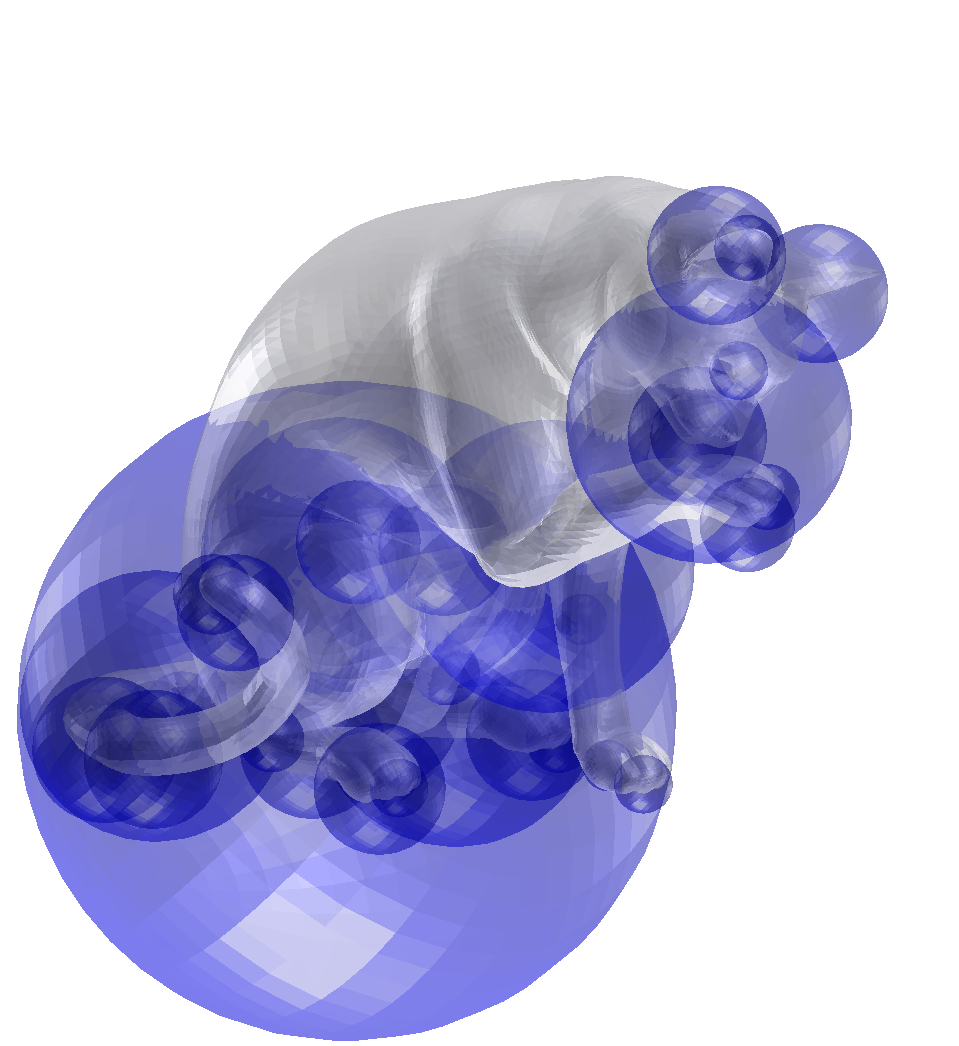
\includegraphics[width=0.18\linewidth]{./fig/eval/cat_dog.png} \hspace{-3mm}
	\label{fig:testshapes:dog}
}
\hspace{-3.5mm}
\subfloat[SURF]{
	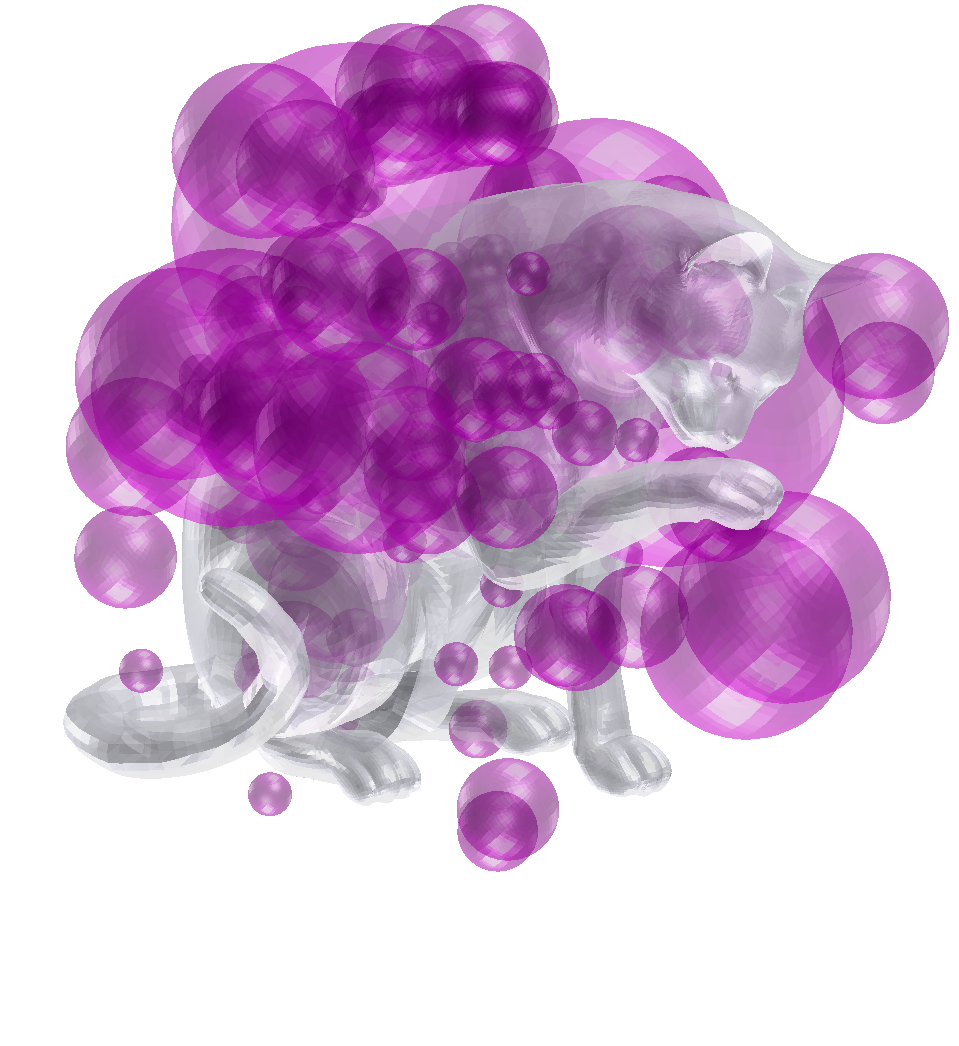
\includegraphics[width=0.18\linewidth]{./fig/eval/cat_surf.png} \hspace{-3mm} 
	\label{fig:testshapes:surf}
}
\hspace{-3.5mm}
\subfloat[Harris]{
	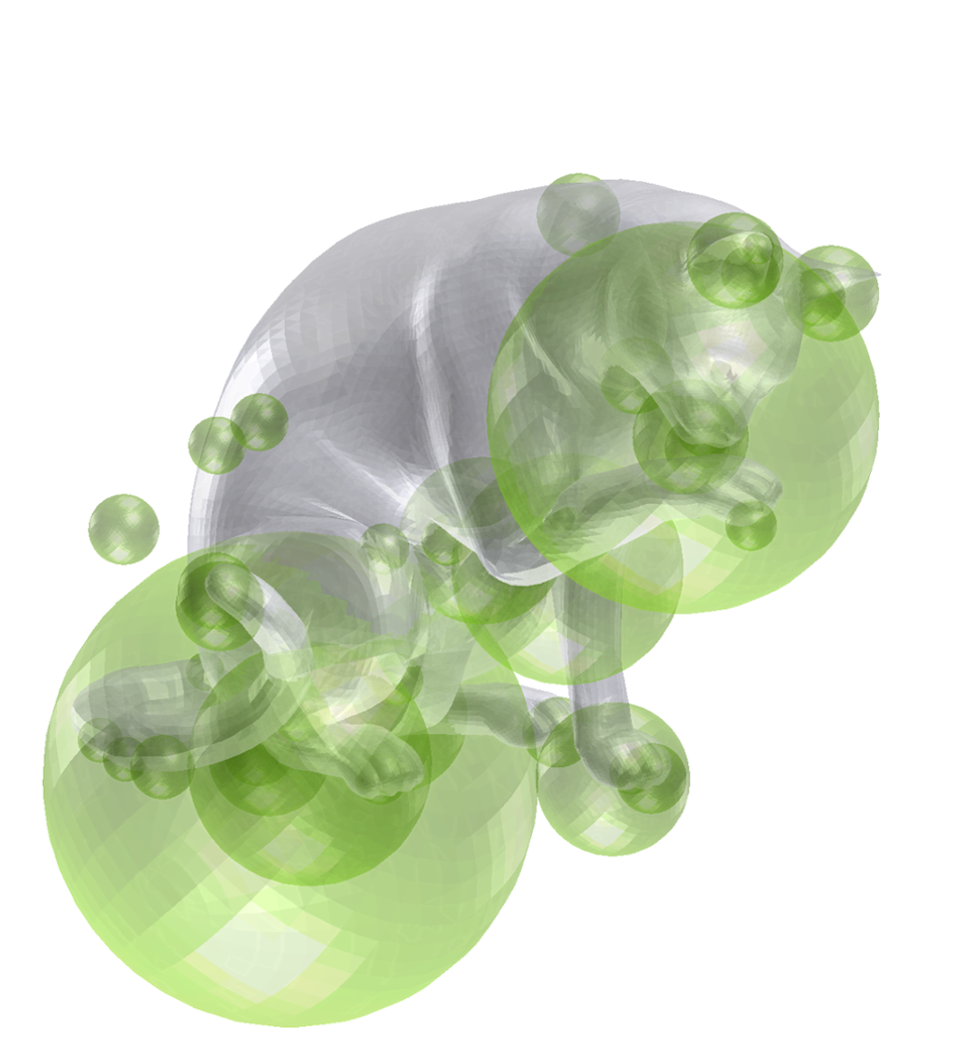
\includegraphics[width=0.18\linewidth]{./fig/eval/cat_harris.png} \hspace{-3mm}
	\label{fig:testshapes:harris}
}
\hspace{-3.5mm}
\subfloat[DoH]{
	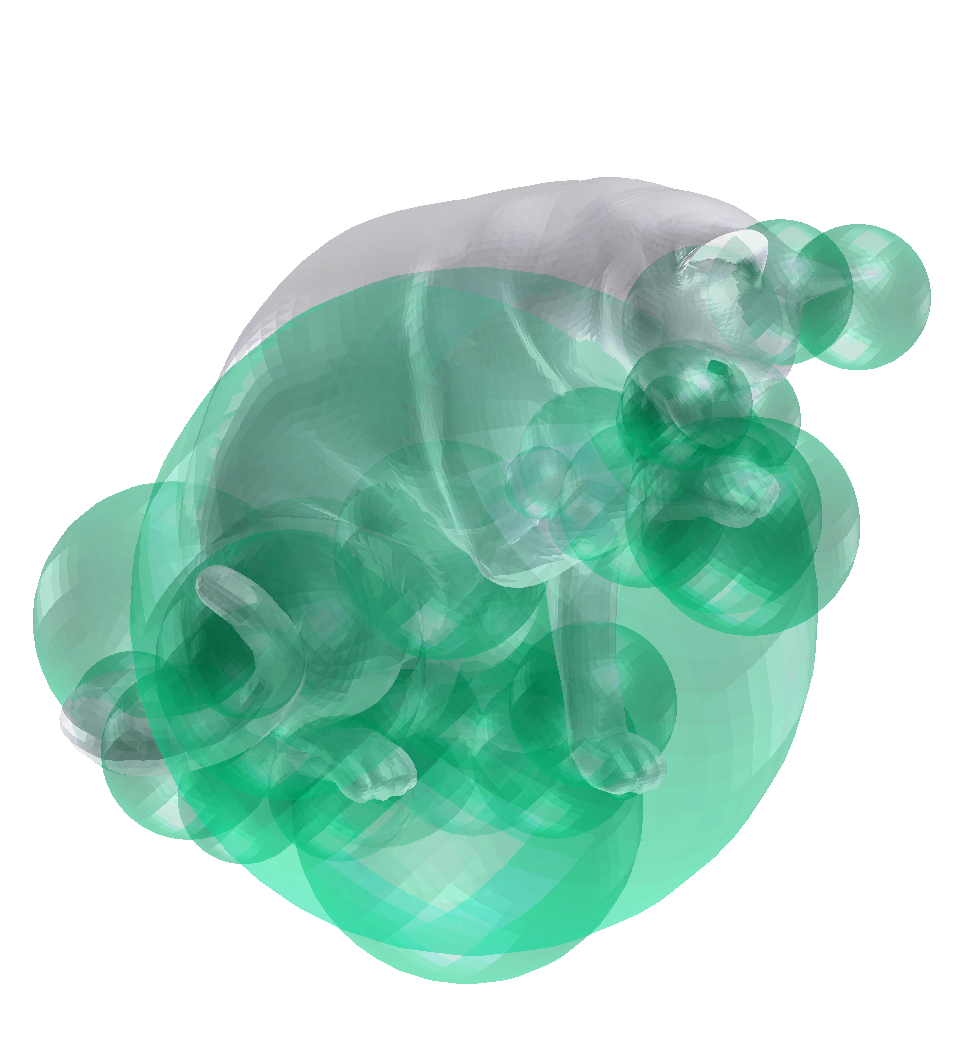
\includegraphics[width=0.18\linewidth]{./fig/eval/cat_hessian.png} \hspace{-3mm}
	\label{fig:testshapes:hessian}
}
\hspace{-3.5mm}
\subfloat[V-FAST]{
	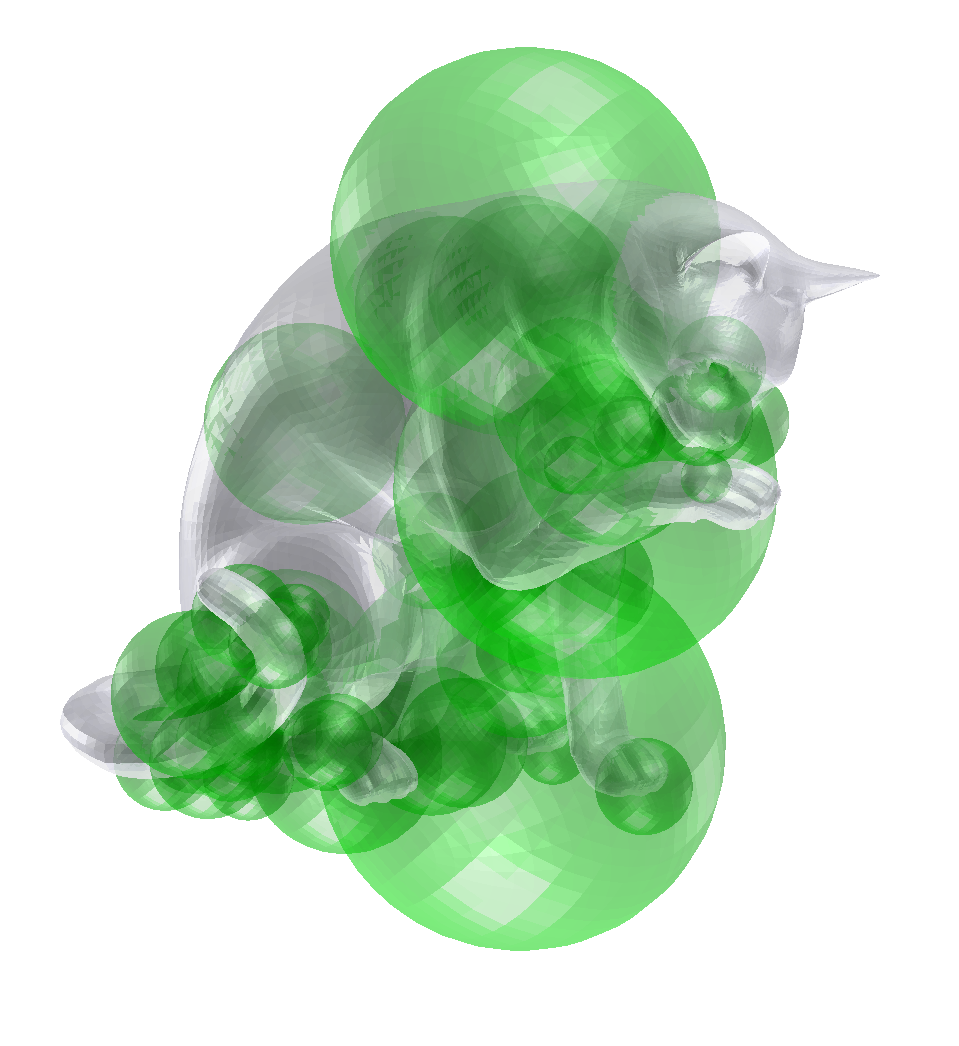
\includegraphics[width=0.18\linewidth]{./fig/eval/cat_fast.png} \hspace{-3mm}
	\label{fig:testshapes:fast}
}
\hspace{-3.5mm}
\subfloat[MSER]{
	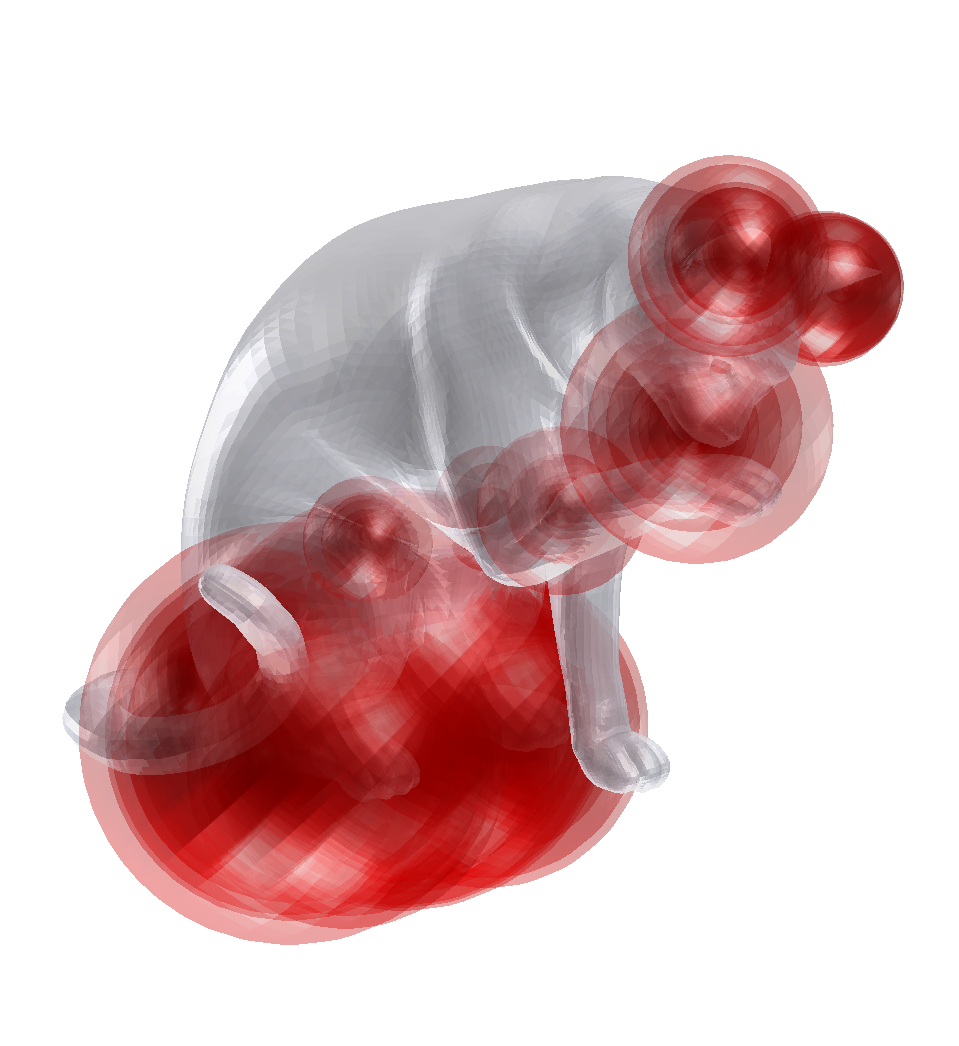
\includegraphics[width=0.18\linewidth]{./fig/eval/cat_mser.png}
	\label{fig:testshapes:mser}
}
\caption{\label{fig:testshapes}Different types of volumetric interest points detected on a test shape.}
\end{figure}

The applications of object detection, recognition and registration are of great importance in computer vision. Much work has been done in solving these problems using appearance on 2D images, helped by the advent of image descriptors such as SIFT and learning-based classifiers such as SVM, and these methods are now reaching maturity. However, advancing geometry capture techniques, in the form of stereo, structured light, structure-from-motion and sensor technologies such as laser scanners, time-of-flight cameras, MRIs and CAT scans, pave the way for the use of shape in these tasks, either on its own or complementing appearance---whilst an object's appearance is a function not only of its texture, but also its pose and lighting, an object's 3D shape is invariant to all these factors, providing robustness as well as additional discriminative power.

Detection and recognition of 3D objects is not new, \eg \cite{Fisher1987}, though such applications have seen a recent resurgence. Approaches range from the local to the global. 
At the global end are those which form a descriptor from an entire object. Such methods generally offer excellent discrimination plus robustness to shape variation, but, since the whole object is required and its extent known, they do not cope well with clutter or occlusion. Also, whilst suitable for recognition, the matching does not provide pose for registration applications. At the other end of the scale are highly local features, such as points. Being completely non-discriminant, such features are usually embedded in a framework that finds geometrical consistency of features across shapes, \eg RANSAC~\cite{Brown2005,Papazov2011}. The geometrical consistency framework makes matching, for detection and recognition, costly, but does provide pose for registration applications, and the local nature of features provides robustness to clutter and partial occlusion. Between these two extremes are those methods that describe local features of limited but sufficiently distinctive scope, thereby gaining the discriminability of global methods and the robustness of local methods. The distribution of such features can be used for effective object detection, recognition and registration. The nature of these hybrid methods is reminiscent of the image descriptors of appearance-based methods, not least in the need for shape features to be chosen at points that are repeatably locatable in different datasets, and whose localities are distinctive. A common and crucial stage of such approaches is therefore the detection of \emph{interest points} to be described. 


This paper aims to conduct a performance evaluation of interest point detectors on scalar volumetric data, as shown in figure~\ref{fig:testshapes}. 
Different from other data-specific 3D interest point detectors for meshes~\cite{Sipiran2011,Glomb2009,Zaharescu2009} or point-clouds~\cite{Aanaes2012,Unnikrishnan2008}, feature detection from scalar volumetric data is more versatile. Such data not only comes directly from volumetric sensors, \eg MRIs, but can also be generated or converted from other three dimensional data such as point clouds, meshes or depth maps, making the evaluation result widely applicable.
In addition, visual saliency of volumetric interest points is defined in a scalar volume but not on a local surface patch. This full three dimensional representation implies that interest points can be located off an object's surface, \eg inside a cavity.
%or inside dense voxels with varying intensities. 
Furthermore, the nature of the data---voxels, the 3D equivalent of pixels---makes repurposing the many 2D interest point detectors for 3D straightforward. The primary quantitative evaluation criterion used here is a novel measure combining both repeatability, based on the number of corresponding points found across two volumes, and the spatial accuracy of correspondences. Detected interest points have a (subvoxel) location and a scale, and distances are computed in this space. This paper also presents a generic evaluation of qualitative characteristics of the interest points.

The following section reviews previous work relevant to interest point detectors and our evaluation framework. Section \ref{sec:detectors} introduces the interest point detectors used in the evaluation experiments, while section \ref{sec:methodology} explains the proposed evaluation methodology.   
Section \ref{sec:experiments} presents the evaluation experiments and their corresponding quantitative and qualitative analyses, before we conclude in section \ref{sec:conclusion}.

%-------------------------------------------------------------------------
\section{Previous work}
\label{sec:previous}

\subsection{Interest point detectors}

The process of interest point detection is the first stage of many computer vision applications, including object detection, recognition and reconstruction. An interest point detector localizes salient points from input visual data for further processing. The detected interest points are typically used to match corresponding points across two or more similar sets of data. 

The majority of earlier studies focus on detecting features on 2D images. The paradigm of 2D interest point detection is now
% matured and 
well studied; we refer the reader to a recent survey~\cite{Tuytelaars2008} for further details. 
%, while recent advancements in data acquisition techniques
%, such as real-time stereo and time-of-flight camera, 
%have greatly improved the availability of 3D shape data. 
Recent advancements in data acquisition techniques have greatly improved the availability of 3D shape data. 
Large scale synthetic and real 3D repositories, such as Google Warehouse~\cite{Lai2010} and the B3DO dataset using the Kinect sensor~\cite{Janoch2011}, have attracted much interest in 3D shape-based computing vision applications. Consequently, various 3D interest point detection techniques have been proposed alongside with this emerging field of computer vision research. 

Existing techniques for 3D interest point detection can be categorized as volume-based or geometry-based detectors, according to the representation of input data. Volume-based detectors operate directly on the pixel/voxel values of volumetric scalar data. This kind of data includes CT scan volumes~\cite{Flitton2010}, binary volumes generated from range data~\cite{Viksten2008} or 3D meshes~\cite{Knopp2010}, and space-time video data~\cite{Koelstra2009,Laptev2005,Willems2008,Yu2010}. Geometry-based interest point detectors extract geometric information (\eg contours, normals or surface patches) and find interest points based on these features. Their input data are usually synthetic meshes~\cite{Glomb2009,Sipiran2011,Zaharescu2009} or point clouds~\cite{Unnikrishnan2008,Aanaes2012}. For geometry-based interest point detectors, recent evaluations have been reported in~\cite{Salti2011} and~\cite{Dutagaci2011}.  
Nevertheless, unlike 2D interest points, performance evaluation of 3D interest points remains a largely unexplored topic. 
This paper aims at the quantitative and qualitative evaluation of volumetric interest point detectors, whose high versatility with respect to data representation enables a much wider coverage of potential applications.

The remainder of this section will review the interest point detectors used in our evaluation, which we divide into two classes based on their definitions of local features.

\subsubsection{Corner Detection}
The first class of interest point detectors aim to find corners (\ie areas of high change in gradient in orthogonal directions) in the input data. 
The Harris interest point detector~\cite{Harris1988} is a classic example of corner detection in 2D, which is still widely used today. It detects interest points by analyzing the eigenvalues of the second moment matrix (first order derivative). Its 3D adaptation has been applied to registration of volumetric CT scans~\cite{Ruiz-Alzola2001,dalvi2010}.  
Building on the success of the traditional Harris detector, Mikolajczyk~\cite{Mikolajczyk2004} developed the scale-covariant\footnote{Covariant characteristics, often (inaccurately) referred to as \emph{invariant} characteristics, undergo the same transformation as the data. We prefer ``covariant'' in order to distinguish truly invariant characteristics.} Harris-Laplace detector by finding Harris corners in the spatial domain which are maxima of the Laplacian in the scale domain. This approach has been extended to space-time interest points for video classification~\cite{Laptev2005}. The SUSAN detector \cite{Smith1997} uses the proportion of pixels in a neighbourhood which are dissimilar to the central pixel to classify corners. The FAST keypoint detector~\cite{Rosten2010} uses the \emph{accelerated segment test} (AST), a relaxed version of SUSAN, for stable corner detection. FAST measures the largest number of contiguous pixels on a circle which are significantly darker, or brighter, than the centre pixel. Without computing the derivative at each pixel, the speed of FAST can be further improved by learning a decision tree classifier for feature detection. Thanks to its efficient run-time performance, several volumetric feature detectors have been applied to space-time volumes classification based on FAST interest points~\cite{Koelstra2009,Yu2010}. 

\subsubsection{Blob Detection}

Lindeberg~\cite{Lindeberg1998} studied scale-covariant interest points using the Laplacian-of-Gaussian kernel (equivalent to the trace of the Hessian), as well as the determinant of the Hessian (DoH).
Lowe~\cite{Lowe2004} approximated the former with a Difference-of-Gaussians (DoG) operator for efficiency. Recently the DoG approach has been applied in 3D, to object detection and recognition of synthetic meshes~\cite{Wessel2006}, volumetric scans~\cite{Flitton2010} and multi-view stereo data~\cite{Pham2011}.

The Hessian-Laplace detector is similar to Harris-Laplace detector; interest points are detected by computing the Hessian matrix from the input data~\cite{Mikolajczyk2004}. The SURF detector~\cite{Bay2008} accelerates computation of the determinant of Hessian through the use of integral images and box filters, since applied to integral volumes of videos~\cite{Willems2008} and binary volumes generated from synthetic 3D mesh models~\cite{Knopp2010}.

While both DoG and SURF are grounded on the approximation of the Laplacian-of-Gaussian kernel,  the \emph{Maximally Stable Extremal Regions} (MSER) interest point~\cite{Matas2004} finds thresholded regions whose areas are maximally stable as the threshold changes. It is therefore inherently multi-scale, as well as invariant to affine intensity variations and covariant with affine transformations. Three dimensional MSER has already been applied to volumetric data, firstly in the context of segmentation of MRIs~\cite{Donoser2006}, then on spatio-temporal data~\cite{Riemenschneider2009}.

\subsubsection{Covariant Characteristics}

Image-based detectors have been made affine-covariant, in order to approximate the perspective distortion caused by projection of 3D world onto the 2D image plane~\cite{Mikolajczyk2002}. Such covariance is \emph{not necessary} with 3D shape data because most shape acquisition techniques are invariant to view point changes, thus affine transformations are not common among datasets. However, objects might have varying poses during data acquisition (\ie translation, rotation and scaling), thus rotation and scale covariance are still essential for processing 3D shape data. In addition, 3D shape data are generally not affected by illumination and lighting conditions, but the quality of shape data is instead determined by the amount of noise and sampling artifacts (\eg holes and occlusions) of the reconstruction process. 

\subsection{Methodologies}
Empirical performance evaluation is a popular pastime in computer vision, and the topic of interest point\footnote{When referring to interest points in the context of methodology, we include image features such as corners, lines, edges and blobs.} detection is no exception. Different approaches of performance evaluations can be categorized according to the evaluation criteria and the source of ground truth interest point locations. 

\subsubsection{Evaluation criteria}
Some methods evaluate performance in the context of a particular task, \eg object recognition~\cite{Shin1999,Dutagaci2011}, 
lacking generality to other applications. Most evaluation frameworks investigate one or more interest point characteristics. 
One such characteristic, important for registration applications, \eg camera calibration, scene reconstruction and object registration, is the accuracy of interest point localization. 
Coelho \etal~\cite{Coelho1992} measure accuracy by computing projective invariants and comparing these with the actual values measured from the scene. Three further measures, including 2D Euclidean distance from detected points to ground truth corner locations (given by line fitting to a grid), are introduced in~\cite{Brand1994}. This approach has been extended to using the distance to the nearest point detected in, and transformed from, another image, \eg~\cite{Schmid2000}. Matching scores for interest points found over location and \emph{scale}~\cite{Laptev2003}
and also \emph{affine} transformations~\cite{Mikolajczyk2004}, have since been proposed.

When used for object detection and recognition, two other important characteristics of interest points are their repeatability and distinctiveness. 
Repeatability is the geometrical stability of the corresponding interest points among multiple input data taken under varying conditions. 
It was proposed and defined by Schmid \etal~\cite{Schmid2000} as the ratio of repeated points to detected points. 
Rosten \etal~\cite{Rosten2010} used the area under the repeatability curve as a function of number of interest points, varied using a threshold on the detector response, in their evaluation. 
When ground truth locations of interest points are given, \eg hand labelled, an alternative measure is the ROC curve~\cite{Bowyer1999}, which takes into account false matches.
Schmid \etal~\cite{Schmid2000} also introduce a quantitative measure of distinctiveness---entropy, or ``information content''.
Alternatively, qualitative visual comparison is used, on test datasets containing a variety of different interest points~\cite{Lindeberg1998,Laptev2005}.
%On the other hand, distinctiveness is more qualitative, and one form of analysis is to present the detector outputs on a test set containing a variety of different interest points, \eg~\cite{LaptevIJCV2005}. A quantitative measure given is entropy, or ``information content''~\cite{SchmidIJCV2000}.

In the context of image-based interest points, performance of detectors are often measured over variations in image rotation, scale, viewpoint angle, illumination and noise level, \eg~\cite{Schmid2000} covers all these factors, as well as corner properties~\cite{Rajan1989}. Efficiency may be a further consideration for applications in which run-time performance is a major concern~\cite{Rosten2010}. Evaluations of 3D interest points not only vary on the above-mentioned criteria, but also on the type of data, such as meshes, space-time volumes, point clouds and space volumes.

It is also worth noting that the distinction between interest point \emph{detectors} and \emph{descriptors}. The latter topic, also well evaluated in 2D, \eg~\cite{Mikolajczyk2005}, has a concept of both correct and incorrect matches, allowing the use of recall-precision as an evaluation criterion.

\subsubsection{Ground Truth Data}
With both localization accuracy and repeatability criteria, the ground truth location of interest points in the scene must be known. The ground truth data can be computed in a variety of ways. Some methods specify the location of interest points in an image, either known by design~\cite{Rajan1989}, or hand labelled by multiple people~\cite{Heath1997}. Other methods match points detected across two or more images. Matching is achieved using planar scenes and computing homographies between images~\cite{Schmid2000}, scenes of known geometry manually registered in each image~\cite{Rosten2010}, scene geometry captured using structured light~\cite{Aanaes2012}, and synthetic data~\cite{Laptev2005}. Ground truth data for 3D interest point evaluations are likewise obtained from manual annotation~\cite{Dutagaci2011}, known projection homography of stereo point clouds~\cite{Aanaes2012} and synthetic shape data~\cite{Salti2011}. 

\section{Detectors}
\label{sec:detectors}

Various volumetric interest points have been proposed in applications such as shape retrieval and classification~\cite{Riemenschneider2009,Flitton2010,Knopp2010,Prasad2011}, medical imaging~\cite{Criminisi2011,Ni2008,Donner2011} and video-based object recognition~\cite{Willems2009,Laptev2005,Yu2010}. Whilst interest point detectors for images have already been studied extensively~\cite{Mikolajczyk2005}, evaluation of volumetric interest points remains largely unexplored. 

This section briefly describes the principles and formulations of the volumetric interest point detectors that we will evaluate.
These include DoG~\cite{Flitton2010}, DoH and Harris-based interest points~\cite{Laptev2005}, SURF~\cite{Willems2008, Knopp2010}, V-FAST~\cite{Yu2010} and MSER~\cite{Donoser2006, Riemenschneider2009}. 

\subsection{Scale-space and subpixel-refinement}
\label{sec:subvoxel}

Scale covariance of interest point detectors is achieved by creating the scale-space of the input volumetric data. An octave of linear scale-space is created by convolving the input volume with a Gaussian smoothing kernel. Such smoothing kernel is applied on the volume recursively to suppress fine-scale structures. In addition, a new octave is created by down-sampling the input volumes from the previous octave. Hence, a series of volumes, with multiple levels of details, is created. The detailed implementation of scale-space, with respect to interest point detection, can be found in~\cite{Lindeberg1998}. 

Scale-space representation is not necessary for MSER because it detects salient regions in different scales. MSER locates interest points by fitting an ellipsoid to the detected salient region~\cite{Matas2004}. For other interest point detectors, saliency responses are computed in all volumes within the scale-space. In addition, the subpixel refinement process of~\cite{Lowe2004} is applied on these detectors; interest points are localized at the subvoxel level by fitting 4D quadratic functions around the local scale-space maxima, and selecting the maxima of those functions instead. 

\subsection{Difference-of-Gaussians (DoG)}
The DoG operator is a blob detection technique for feature localization popularized by the SIFT algorithm~\cite{Lowe2004}.    
DoG approximates the Laplacian of Gaussian filter, which detects features of a particular size. 
The saliency response of DoG detector $S_{\textrm{DoG}}$ is computed by subtracting two Gaussian smoothed volumes, usually adjacent scale-space representations, of the same signal and taking the absolute values of this.
Interest point are detected at the \emph{4D local maxima} (both 3D space and scale) in $S_{\textrm{DoG}}$ within each octave of $\mathbf{V}(\mathbf{x},\sigma_s)$:
\begin{equation}
S_{\textrm{DoG}}(x,y,z;\sigma_s) = |V(x,y,z;\sigma_s) - V(x,y,z;\sigma_{s-1})|
\end{equation}
where $V(x,y,z;\sigma_s)$ is the scale-space representation of the input volumetric data at scale $\sigma_s$.

\subsection{Harris}
Harris corner detector examines changes of intensity due to shift in a local window, interest points are detected at positions where large changes are observed in all directions~\cite{Harris1988}. While the first 3D extension~\cite{Laptev2005} of the traditional Harris corner detector uses separate scale parameters for the heterogeneous space and time axes, here one scale parameter $\sigma_s$ is shared among three homogeneous spatial axes. 
The second-moment matrix $\mathtt{M}$ is computed by smoothing the first derivatives of the volume in scale-space $\mathbf{V}(\mathbf{x};\sigma_s)$ by a spherical Gaussian weight function $g(\cdot;\sigma_\textrm{Harris})$, thus: 

\begin{equation}
\begin{array}{rcl}
\mathbf{V}_x(\mathbf{x};\sigma^2_s) &= &\displaystyle\frac{\partial \mathbf{V}(\mathbf{x};\sigma^2_s)}{\partial x} \\
\mathbf{V}_y(\mathbf{x};\sigma^2_s) &= &\displaystyle\frac{\partial \mathbf{V}(\mathbf{x};\sigma^2_s)}{\partial y} \\
\mathbf{V}_z(\mathbf{x};\sigma^2_s) &= &\displaystyle\frac{\partial \mathbf{V}(\mathbf{x};\sigma^2_s)}{\partial z}
\end{array}
\end{equation}
\begin{equation}
\mathtt{M} = g(\cdot;\sigma_\textrm{Harris}) \ast \left[
\begin{array}{ccc}
\mathbf{V}^2_x & \mathbf{V}_x\mathbf{V}_y & \mathbf{V}_x\mathbf{V}_z \\
\mathbf{V}_x\mathbf{V}_y & \mathbf{V}_y^2 & \mathbf{V}_y\mathbf{V}_z \\
\mathbf{V}_x\mathbf{V}_z & \mathbf{V}_y\mathbf{V}_z & \mathbf{V}^2_z \\
\end{array}
\right]
\label{eq:harris_2ndmoment}
\end{equation}
where $\mathbf{V}_x$,$\mathbf{V}_y$,$\mathbf{V}_z$ denote the partial derivatives of the volume in scale-space $\mathbf{V}(\mathbf{x};\sigma_s)$ along $x$, $y$ and $z$ axes respectively. 
The matrix $\mathtt{M}$ describes the autocorrelation along different directions in a local neighbourhood of size $\sigma_s$. 

The saliency $S_\textrm{Harris}$ is computed from the determinant and trace of $\mathtt{M}$, as follows:
\begin{equation}
S_\textrm{Harris} = \sigma_{s}^3 \:\mathrm{det}(\mathtt{M}) - k\:\mathrm{trace(\mathtt{M})}^3
\label{eq:harriscorner}
\end{equation}

A user defined threshold $k$ controls the rejection of edge points.
Each saliency response $S_\textrm{Harris}$ is normalized by its scale $\sigma_s$. The window size $\sigma_\textrm{Harris}$ is proportional to expected feature scales $\sigma_s$ by a factor of $0.7$ as suggested in~\cite{Mikolajczyk2004}. 
Candidate interest points are located at coordinates $(x,y,z)$ where the second-moment matrix 
\begin{equation}
\mathtt{M}(x,y,z,\sigma_\textrm{Harris};\sigma_s)
\end{equation} 
has large eigenvalues $\lambda_1, \lambda_2, \lambda_3$. Interest point are hence the 4D local maxima in the scale-space of $S_{\textrm{Harris}}$. Locations of interest points are refined using the sub-voxel refinement method described in \ref{sec:subvoxel}.

\subsection{Determinant of Hessian (DoH)}
\label{sec:doh}
The DoH interest point is similar to the Harris detector with respect to formulation~\cite{Lindeberg1998}; instead of computing the second-moment matrix $\mathtt{M}$, it is based on the Hessian matrix $\mathtt{H}$ in equation \ref{eq:hessianmatrix}:
\begin{equation}
\mathtt{H} = 
\left[
\begin{array}{ccc}
\mathbf{V}_{xx} & \mathbf{V}_{xy} & \mathbf{V}_{xz} \\
\mathbf{V}_{yx} & \mathbf{V}_{yy} & \mathbf{V}_{yz} \\
\mathbf{V}_{zx} & \mathbf{V}_{zy} & \mathbf{V}_{zz} 
\end{array}
\right]
\label{eq:hessianmatrix}
\end{equation}
where $\mathbf{V}_{xy}$ denotes the second derivative of the volume at scale $\sigma_s$, along $x$ and $y$ axes: 
\begin{equation}
\mathbf{V}_{xy} = \frac{\partial \mathbf{V}(\mathbf{x};\sigma_s)}{\partial x \partial y}
\label{eq:hessiandiverative}
\end{equation}
The saliency response is the scale-normalized determinant of Hessian matrix $\mathtt{H}$:
\begin{equation}
S_{\textrm{Hessian}} = \sigma^3_s \:\mathrm{det}(\mathtt{H})
\label{eq:hessiansaliency}
\end{equation}
Similar to Harris and DoG, the interest points are located at the 4D scale-space local maxima of $S_\textrm{Hessian}$.

\subsection{SURF}
Speeded up robust features (SURF) is a feature extraction algorithm optimized for efficiency~\cite{Bay2008}. The 3D, volumetric version of SURF was first introduced in~\cite{Willems2008} for video classification. Recently, it was used in a 3D shape object recognition task~\cite{Knopp2010}.

SURF is an efficient approximation of the DoH detector. Second-order derivatives of Gaussians in the DoH detector are approximated by six Haar wavelets (\ie box filters). Convolutions of the Haar wavelets can be greatly accelerated using integral videos/volumes. The saliency response of 3D SURF is similar to the aforementioned DoH detector. 

\subsection{V-FAST}

Building on the success of the FAST corner detector~\cite{Rosten2010}, V-FAST~\cite{Yu2010} and FAST-3D~\cite{Koelstra2009} have been proposed for video-based object classification. The V-FAST algorithm performs accelerated segment tests on three orthogonal circles along $xy$, $xz$ and $yz$ planes. The saliency score is computed by maximizing the threshold $t$ that makes at least $n$ contiguous voxels brighter or darker than the nucleus voxel by $t$, thus: 
\begin{equation}
AST_{xy}(n,t) = \left\{
\begin{array}{lc}
t & \textrm{if}~~||v_\textrm{nucleus} > \mathbf{c}_{xy} + t || \ge n \\
t & \textrm{if}~~||v_\textrm{nucleus} < \mathbf{c}_{xy} - t || \ge n \\
0 & \mbox{ otherwise }
\end{array}
\right.
\label{eq:fastast}
\end{equation}
\begin{equation}
S^{xy}_\textrm{vfast} = \mathrm{max}(AST_{xy}(n,t))
\label{eq:fast}
\end{equation}
\begin{equation}
S_\textrm{vfast} = \sqrt{(S^{xy}_\textrm{vfast})^2+(S^{xz}_\textrm{vfast})^2+(S^{yz}_\textrm{vfast})^2}
\label{eq:fastverall}
\end{equation}
$\mathbf{c}_{xy}$ denotes the voxels on an $xy$-circle centered at $v_\textrm{nucleus}$. The combined saliency response $S_{\textrm{vfast}}$ is the Euclidean norm of saliency scores on the three planes in equation \ref{eq:fastverall}. Interest points are detected at the local maxima in $S_{\textrm{vfast}}$ over both translation and scale, with at least two non-zero responses in $AST_{xy}(n,t)$, $AST_{xz}(n,t)$ and $AST_{yz}(n,t)$.

\subsection{MSER}
The maximally stable extremal regions (MSER) detector is a region-based blob detection technique proposed by Matas \etal~\cite{Matas2004}. Extremal regions are the connected components of a thresholded input data (image/volume); the maximally stable regions are selected from a set of nested extremal regions obtained using different thresholds. The extremal regions of an input volume can be enumerated efficiently using the union-find algorithm which has a worst case of $O(N\log\log N)$~\cite{Matas2004}, where $N$ is the number of pixels/voxels. Being inherently advantageous for volumetric interest point detection (\eg robust to rotation and scale changes), MSER has been applied to detection of volumetric salient regions~\cite{Donoser2006,Riemenschneider2009}.

Normally an ellipsoid is fitted to each maximally stable region from the input data~\cite{Matas2004}, the position and scale of MSER interest points being represented by the centres and radii of such ellipsoids respectively. In this work a sphere is fitted to the stable regions instead, making the interest points compatible with the proposed evaluation framework.

\begin{figure}[ht]
\centering
\subfloat[Mesh]{
	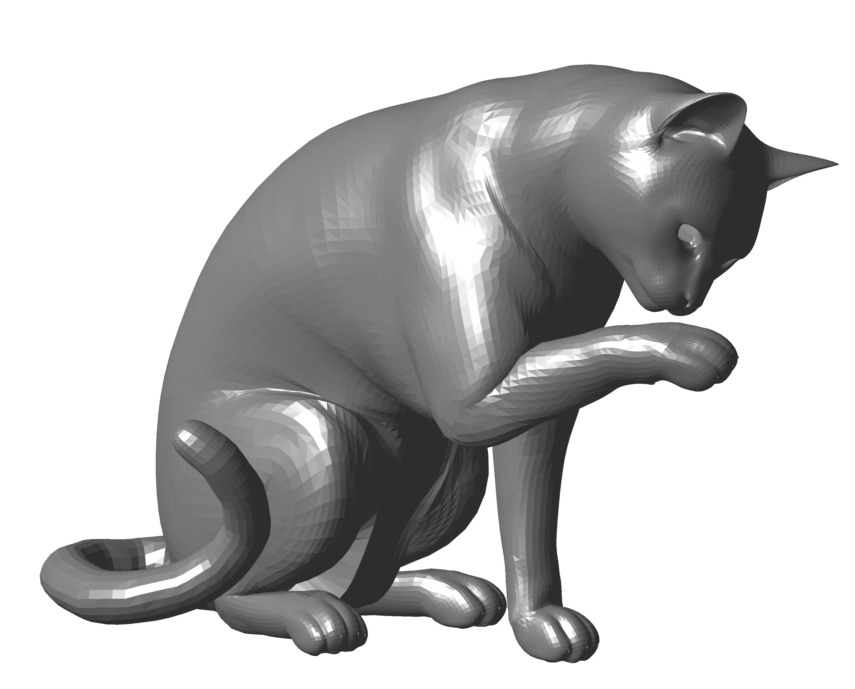
\includegraphics[height=0.22\linewidth]{./fig/eval/cat_mesh.png} 
}
\subfloat[Point cloud]{
	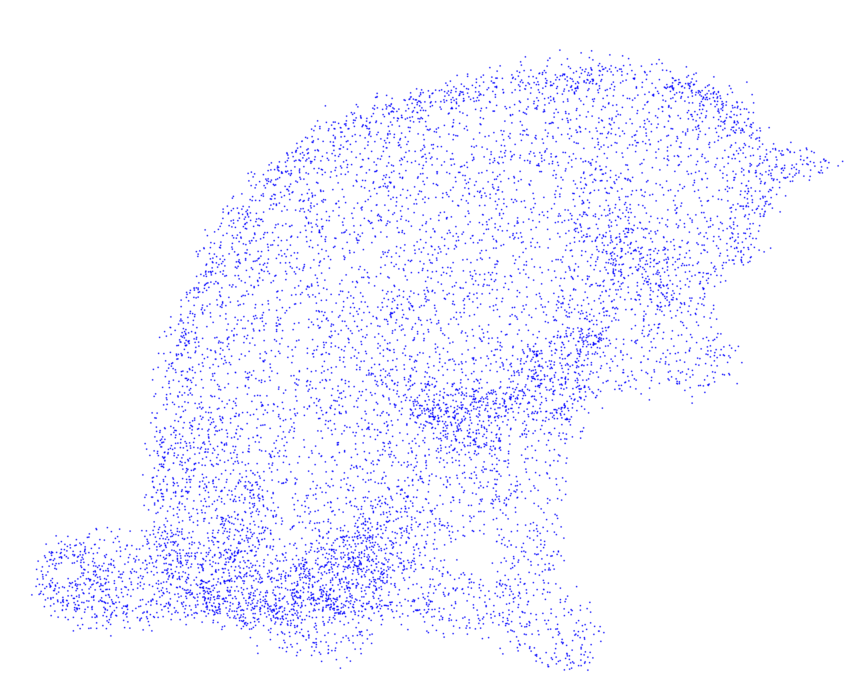
\includegraphics[height=0.22\linewidth]{./fig/eval/cat_points.png}
}
\subfloat[Voxel array]{
	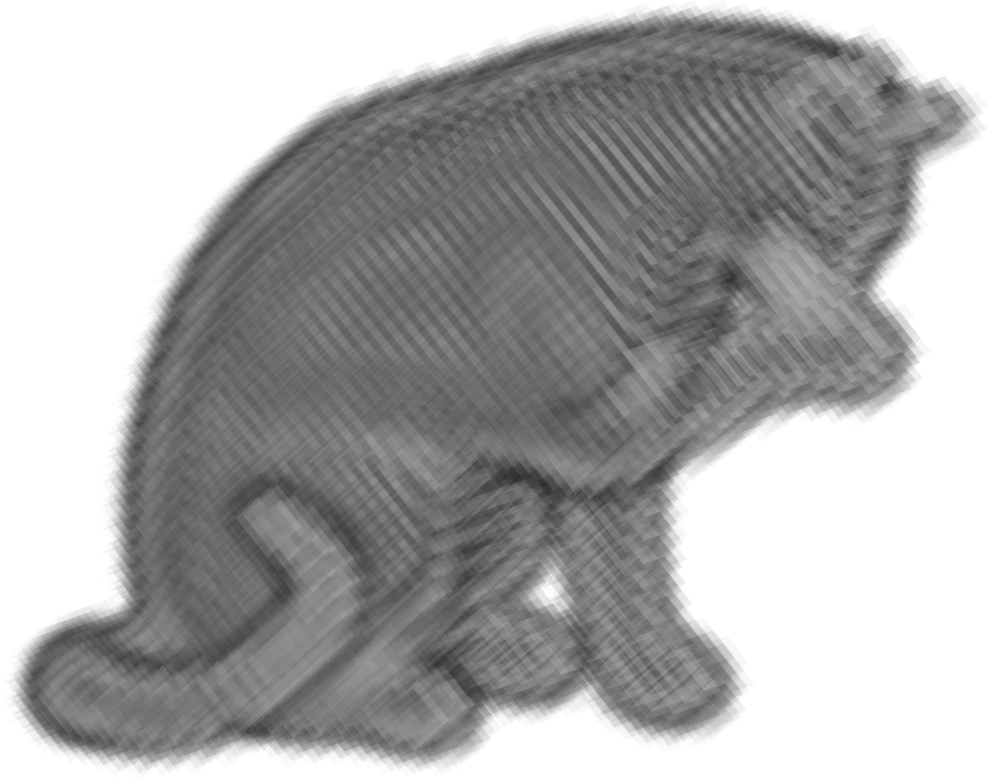
\includegraphics[height=0.2\linewidth]{./fig/eval/cat_volume.png}
}
\caption{\textbf{Mesh to volume conversion}. \emph{Left to right}: mesh, point cloud and voxel array.} 
\label{fig:vol_conversion}
\end{figure}


\section{Methodology}
\label{sec:methodology}

The traditional repeatability ratio measures the repeatability of interest point detectors at a single, predefined accuracy; it is therefore not only sensitive to the choice of matching distance threshold, but also gives little indication of localization accuracy, \ie the closeness of corresponding interest points, for correspondences, other than that they fall within the threshold. As such, a single repeatability ratio is not sufficient to describe the performance of interest point detectors for various applications with different accuracy requirements. 

On the other hand, real matching accuracy, \eg ROC curves in \cite{Bowyer1999}, requires hand crafted point-to-point groundtruth correspondences. This approach is therefore difficult to generalize to large, realistic evaluation datasets such as point clouds from multi-view stereo systems.   

Whilst previous evaluations have focused on either localization accuracy or repeatability, we combine the two performance metrics into a single score. The proposed combined score is computed based on repeatability ratio with respect to varying accuracy requirements. This section explains the combined score used in our evaluation.   

\subsection{Localization accuracy}

An interest point is considered as a sphere at coordinates $[P_x, P_y, P_z]$ with radius $P_s$ given by its scale. A vector $\mathbf{P}$ is used to describe this interest point by combining its spatial location and scale, thus: 
\begin{equation}
\mathbf{P} = [P_x,~P_y,~P_z,~f\log(P_s)]^\mathsf{T}
\label{eq:loc_vec}
\end{equation}
The logarithm of scale is used to remove multiplicative bias across detectors, and since spatial location and scale are not fully commensurate, a parameter $f$ is introduced to weight the importance of scale to the distance function.

A key component of the proposed evaluation score is the distance metric for measuring the closeness of two corresponding interest points with respect to their locations and scales. In this work the Euclidean norm is used:
\begin{equation}
D(\mathbf{P}, \mathbf{Q}') = ||\mathbf{P} - \mathbf{Q}'||
\label{eq:matchdistance}
\end{equation}
% A key component of the proposed evaluation score is the distance metric for measuring the closeness of two corresponding interest points with respect to their locations and scales. 
%An interest point $\mathbf{P}$ is represented by a sphere at coordinates $[P_x, P_y, P_z]$ with radius $P_s$ given by scale.   
%\begin{equation}
%D(\mathbf{P}, \mathbf{Q}') = ||\mathbf{P} - \mathbf{Q}'||_2
%\label{eq:matchdistance}
%\end{equation}
%A key component of the proposed evaluation score is the distance metric used to measure the closeness of two corresponding interest points with respect to their locations and scales:
%\begin{equation}
%\mathbf{P} = [P_x,~P_y,~P_z,~f\log P_s]^\mathrm{T}
%\label{eq:loc_vec}
%\end{equation}
%The log of scale is used to remove multiplicative bias across detectors, and since spatial location and scale are not fully commensurable, a parameter $f$ is introduced to balance the importance of scale to the distance function. 
where $\mathbf{P}$ is the coordinates of an interest point found in the volume, $V_P$, and $\mathbf{Q}'$ is the point $\mathbf{Q}$ found in volume $V_Q$, transformed into the coordinate frame of $V_P$ using a known ground truth homography. The evaluation score is based on the distance of an interest point to the nearest transformed interest point in equation \ref{eq:metricNN}:
\begin{equation}
D(\mathbf{P}, \mathcal{Q}') = \min_{\mathbf{Q}'_j \in \mathcal{Q}'}D(\mathbf{P}, \mathbf{Q}'_j)
\label{eq:metricNN}
\end{equation}
where $\mathcal{Q}' = \{\mathbf{Q}'_j\}_{j=1}^{q}$, the set of $q$ transformed interest points found in $V_Q$.

\subsection{Repeatability}
Schmid \etal~\cite{Schmid2000} defined repeatability as the ratio of correspondences to points:
\begin{equation}
R_\textrm{ratio}(\mathcal{P}, \mathcal{Q}', \delta) = \frac{\sum_{i=1}^p H(D(\mathbf{P}_i, \mathcal{Q}') - \delta)}{\min(p, q)}
\label{eq:repeatratio}
\end{equation}
where $\mathcal{P} = \{\mathbf{P}_i\}_{i=1}^{p}$, the set of $p$ interest points found in $V_P$, and $\delta$ is a user provided distance threshold. 
The Heaviside step function $H(\cdot)$ returns $1$ when the input is positive, $0$ otherwise.
This repeatability measure favours dense interest points over accurate but sparse interest points~\cite{Willis2009}. 
However, the fairness of our evaluation is not affected because fully-overlapped object pairs are used in the experiments.
%In addition, the symmetry of the combined $R_\textrm{area}$ score~\ref{eq:rptarea} cancels out the effect of differences in interest points' density.

\subsection{Combined score}
Rosten \etal~\cite{Rosten2010} computed the area under $R_\textrm{ratio}$ as a function of the number of interest points, varied using a contrast threshold on the detector. We use the same idea, but computing $R_\textrm{ratio}$ as a function of the distance threshold, $\delta$. The score therefore increases both if a higher proportion of points are matched, and also if matches are more accurate. We also compute a symmetric score, by computing the average score across two matching directions, using $V_P$ and $V_Q$ as the reference frames respectively, in order to  cancel out the effect of differences in interest point density between the volumes. This score is given as the area under the $\delta$ \emph{vs} $R_\textrm{ratio}$ curve within a maximum matching distance $D$, thus:
\begin{equation}
R_\textrm{area}=\frac{1}{2D}\int_{0}^{D}R_\textrm{ratio}(\mathcal{P}, \mathcal{Q}', \delta) + R_\textrm{ratio}(\mathcal{Q}, \mathcal{P}', \delta) ~ \textrm{d}\delta
\label{eq:rptarea}
\end{equation}
Our $R_{\textrm{area}}$ score is advantageous over traditional repeatability, as it reflects both repeatability and accuracy of interest points in one measurement. 



\section{Evaluation}
\label{sec:experiments}
In this section we perform a comprehensive evaluation of the volumetric interest point detectors, investigating their performance under different variations of input data. 
%The robustness of interest points are indicated by the corresponding $R_{\textrm{area}}$ scores under each variation. Repeatability of interest points are analyzed qualitatively using real-life shape data (e.g. MRIs and multi-view stereo). Furthermore, by comparing different evaluation results, the relationship between volumetric interest points and image-based interest points is studied.

\subsection{Test data}
\label{sec:testdata}
Three different datasets are used in our evaluation. Two of these are synthetic, as large sets of real, registered, 3D data are not commonly available. Synthetic data are used because we can generate new test data with varying noise levels, transformations and sampling density with accurate ground-truths for evaluation. It is shown in figure~\ref{fig:graph2} that synthetic and real testing data are comparable in our evaluation. 

The first set, \textbf{Mesh}, contains 25 shapes (surface meshes) chosen from the Princeton Shape Benchmark~\cite{Shilane2004} and \emph{TOSCA}~\cite{Bronstein2008} dataset. This selection contains a wide range of geometric features, from coarse structures to fine details, as illustrated in figure \ref{fig:sampleshapes}. Point clouds are created by sampling 3D points, with a uniform distribution, over the surfaces of the meshes. Gaussian white noise is added to the points to simulate measurement errors introduced during 3D shape acquisition. 
The point clouds are then \emph{voxelized} to volumetric data using kernel density estimation with a Gaussian kernel $g(\cdot,\sigma_{KDE})$, as illustrated in figure~\ref{fig:vol_conversion}.
%This conversion process allows sampling density and noise to be varied when generating the volumes.
Finally, a linear scale-space $\mathbf{V}(\mathbf{x};\sigma_s)$ is created from each volume, in order to detect shape features at different scales. All shapes in the dataset undergo this conversion process. 

The \textbf{MRI} dataset consists of two synthetic MRI scans of a human brain, generated from BrainWeb simulated brain database~\cite{Cocosco1997}, with given ground truth homography ($20^{\circ}$ rotation and $20$ voxel translation) between the two scans
%The ground truth registration (homography) between the two MRI scans is given for performance evaluation.

The third dataset, \textbf{Stereo}, is a series of $16$ point clouds of $8$ objects from the Toshiba CAD model point clouds dataset \cite{Pham2011}, which is captured using a multi-view stereo system~\cite{Vogiatzis2011}.  Relative transformations are computed by aligning each point cloud with a reference model using the \emph{iterative closest point} algorithm \cite{Besl1992}. The same voxelization technique is used to convert stereo point clouds to volumetric data.

In \textbf{Mesh} and \textbf{Stereo} datasets, high-intensity voxels are located at the object surface, leaving the interior of the shapes hollow as low-intensity voxels. In contrast, the interior of the \textbf{MRI} data is filled with voxels of differing intensity. The experimental results demonstrate the detector behaviours in these two voxelization scenarios.

While the synthetic shape instances of the same object completely overlap one another, avoiding bias to the repeatability score~\cite{Willis2009}, the real stereo data contains occlusions (the underside of each object, which varied across instances, was not captured), as well as uneven sampling density and generally more sampling noise. The applicability to real applications of our performance evaluation using synthetic data will therefore be tested by comparing the results on the {\textbf Mesh} dataset with those on the {\textbf Stereo} dataset. 


%\begin{figure}[ht]
%\centering
%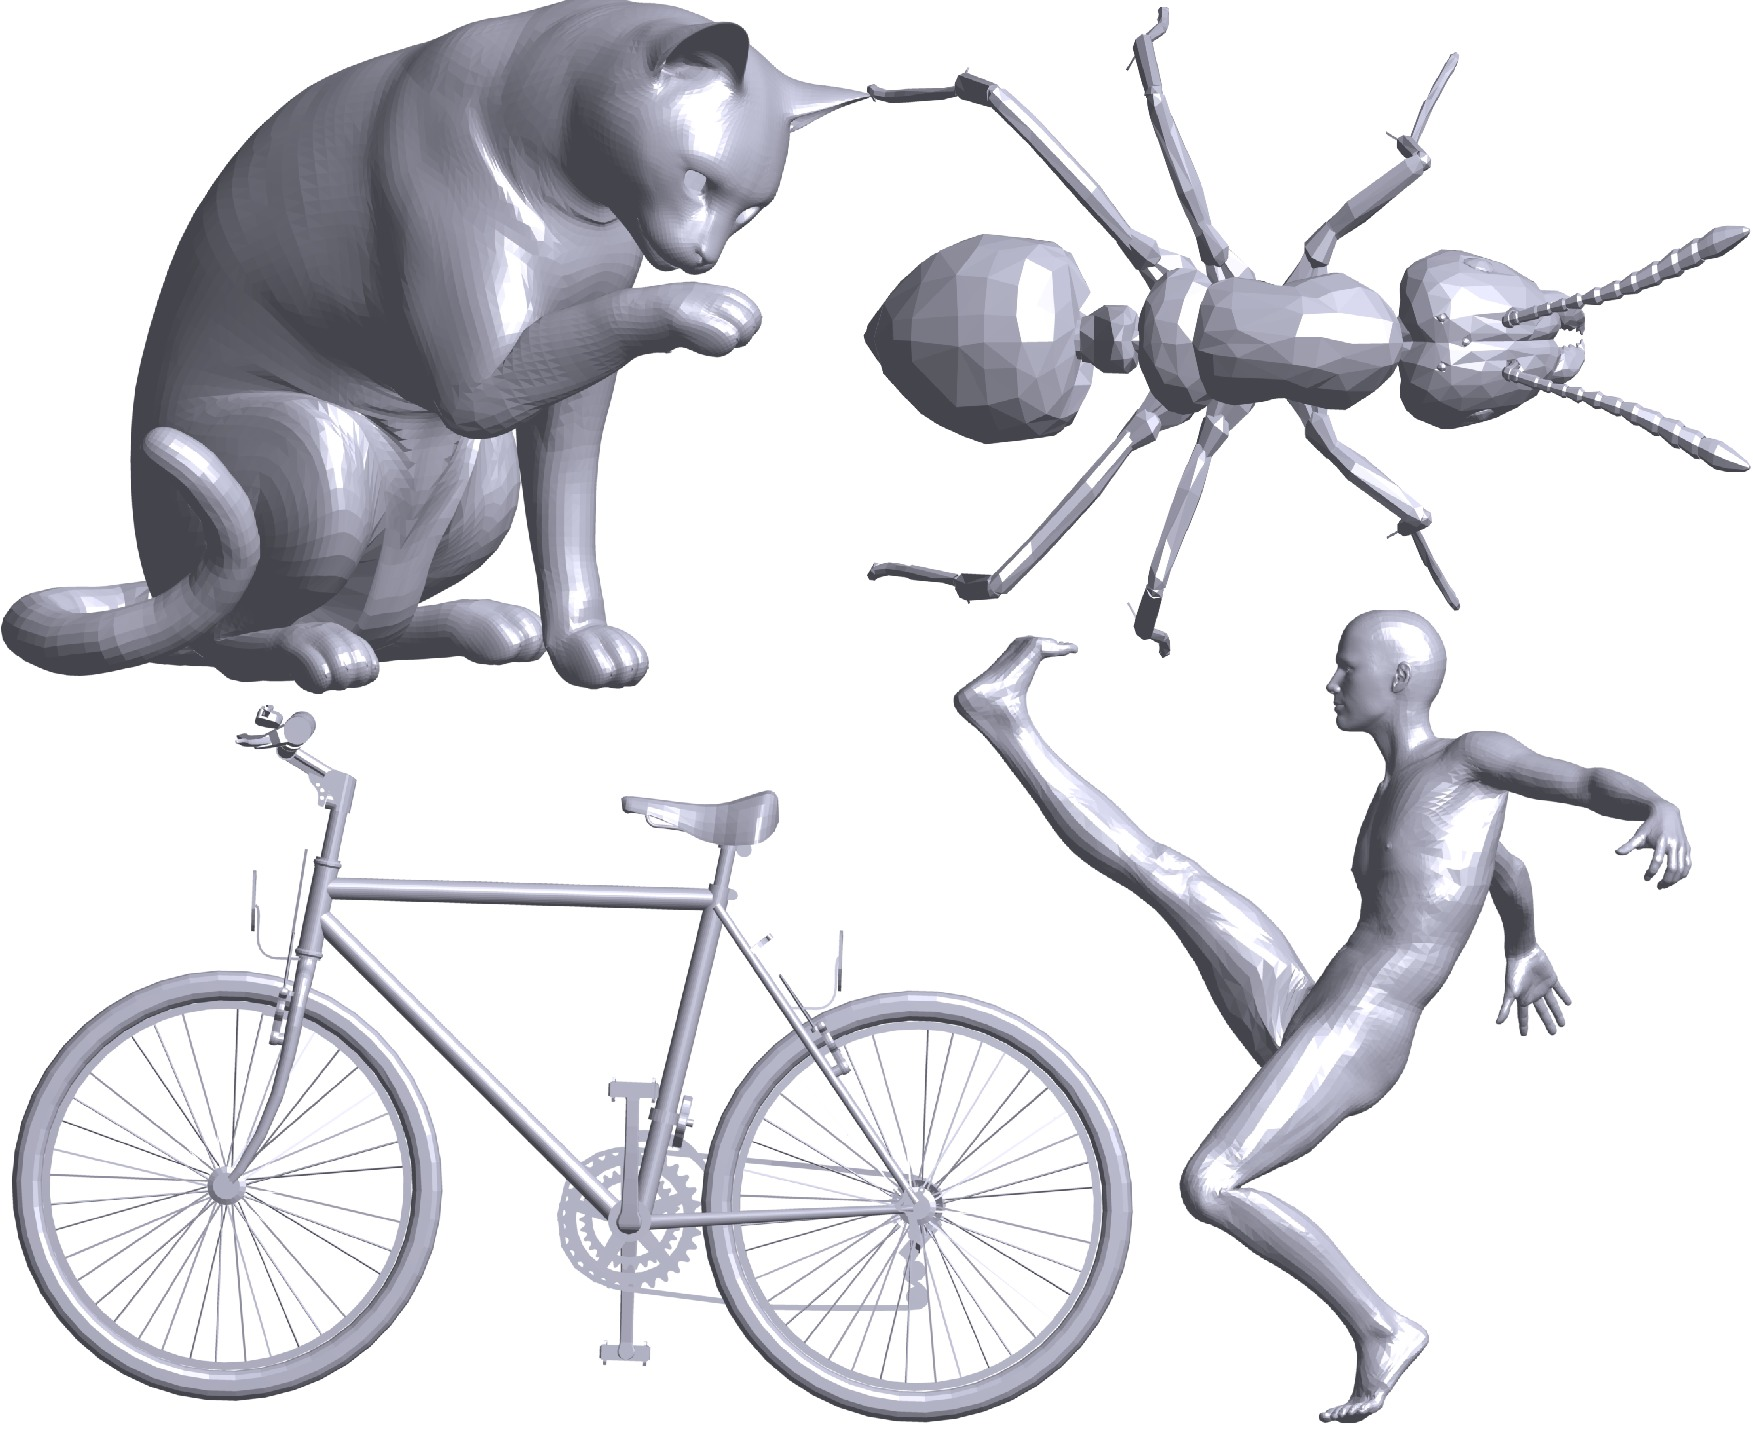
\includegraphics[width=0.75\linewidth]{./fig/eval/sampleshape.pdf}
%\caption{Example shapes taken from the \textbf{Mesh} dataset.} 
%\label{fig:sampleshapes}
%\end{figure}

\begin{figure}
	\begin{subfigure}[t]{0.19\linewidth} \centering
		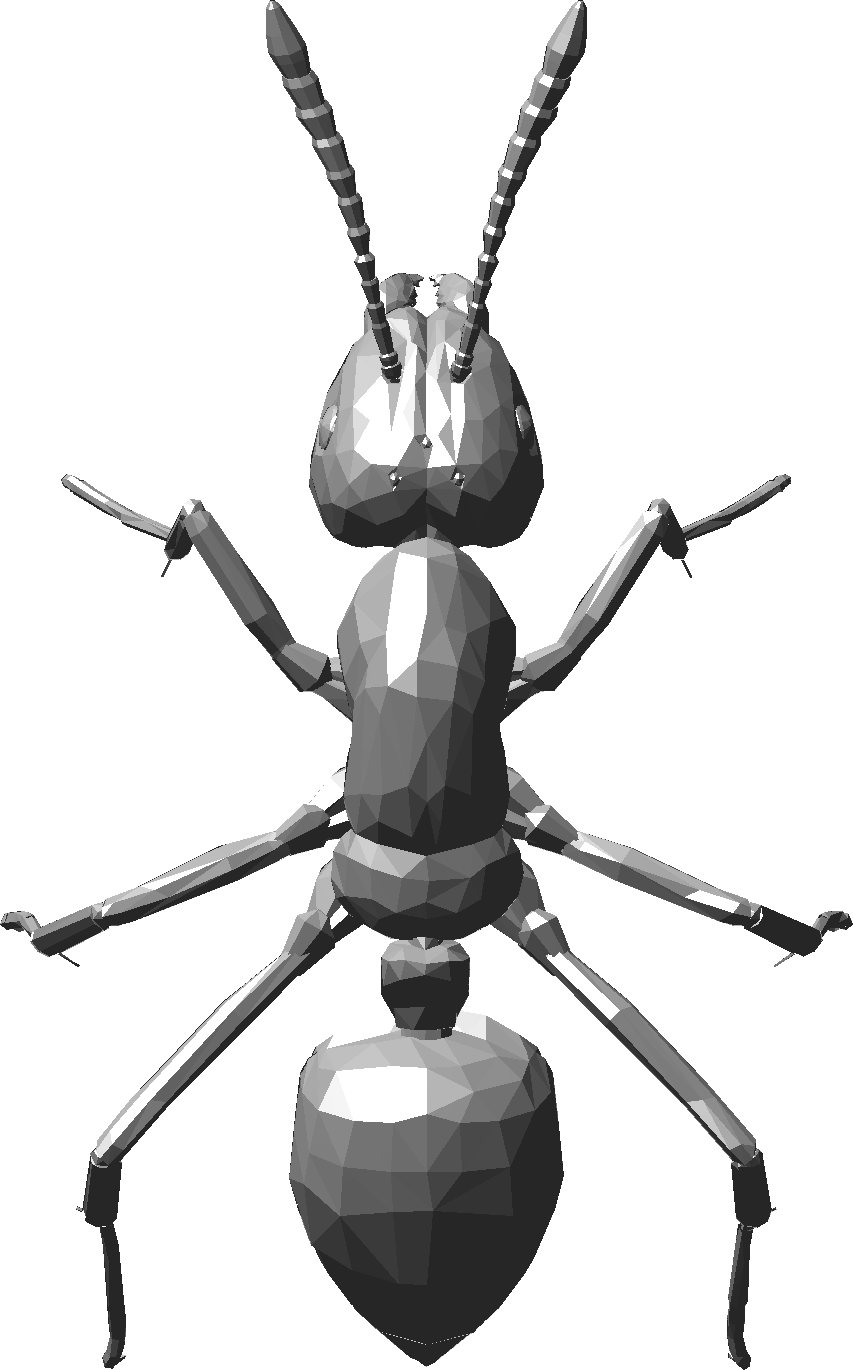
\includegraphics[width=0.7\linewidth]{./fig/eval/01ant.png}  
		\caption{Ant} 	
	\end{subfigure}
	\begin{subfigure}[t]{0.19\linewidth} \centering
		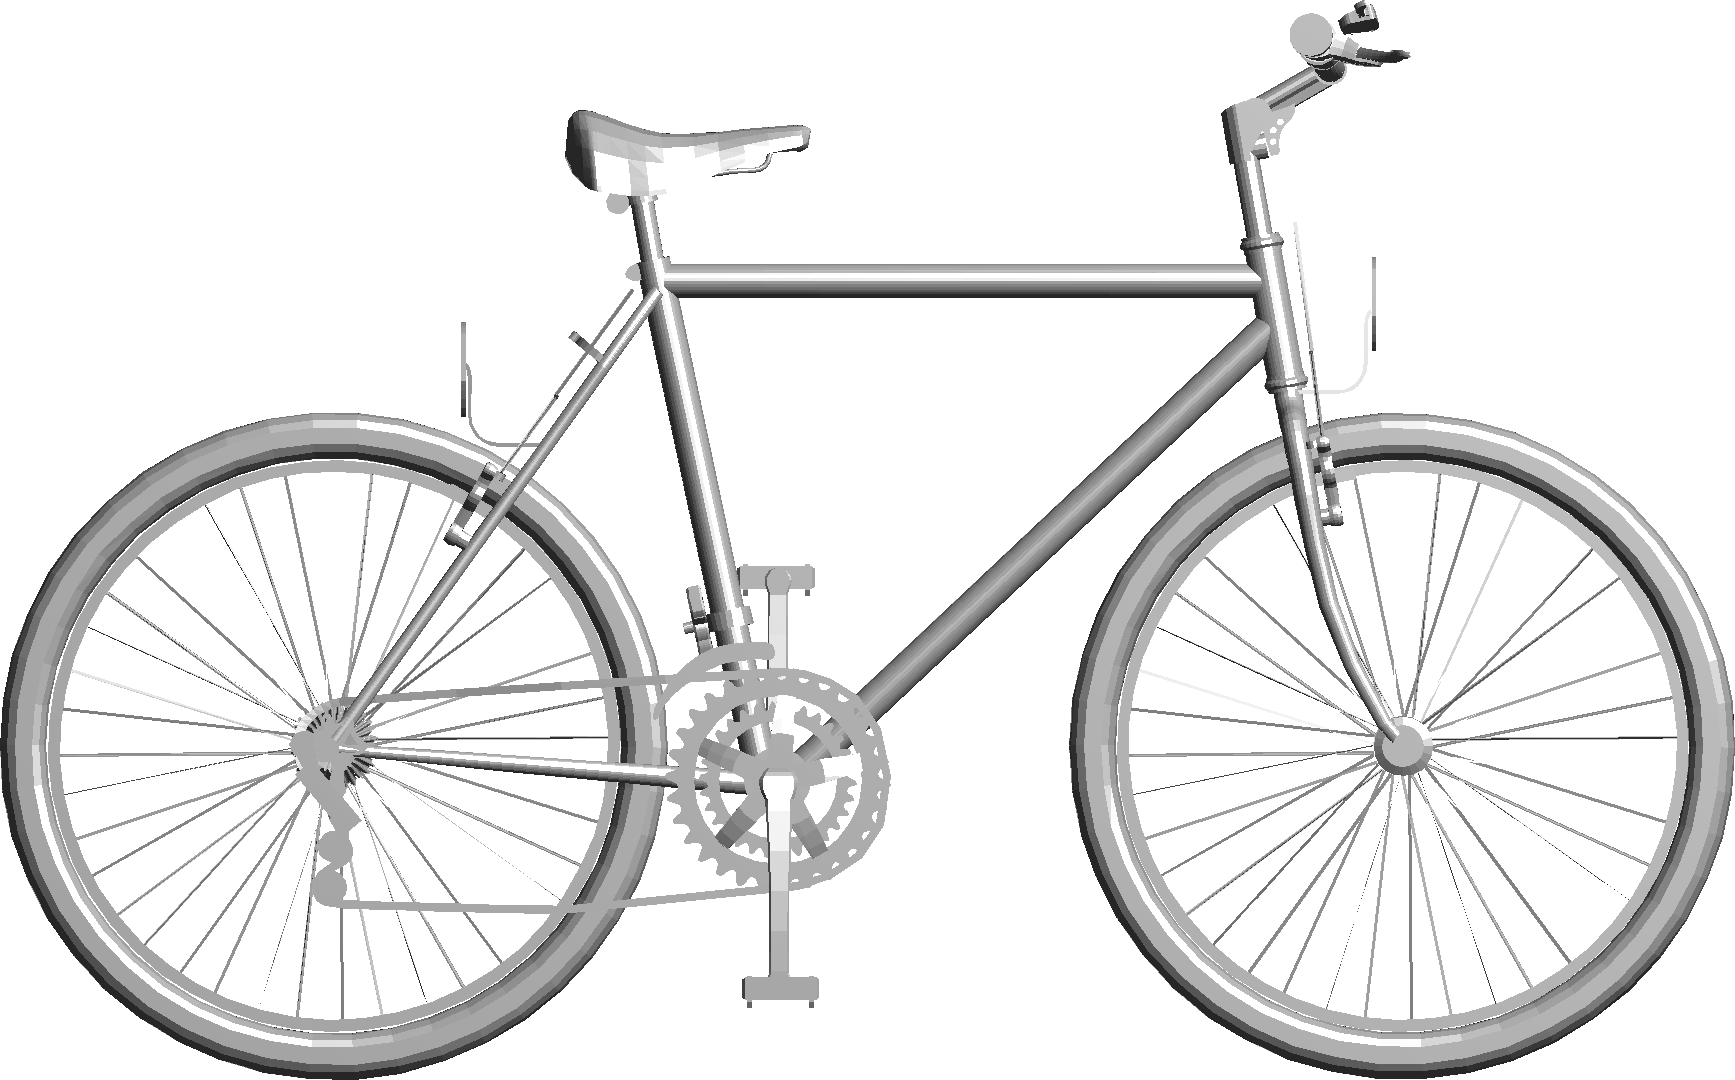
\includegraphics[width=1\linewidth]{./fig/eval/02bicycle.png}  
		\caption{Bicycle} 	
	\end{subfigure}
	\begin{subfigure}[t]{0.19\linewidth} \centering
		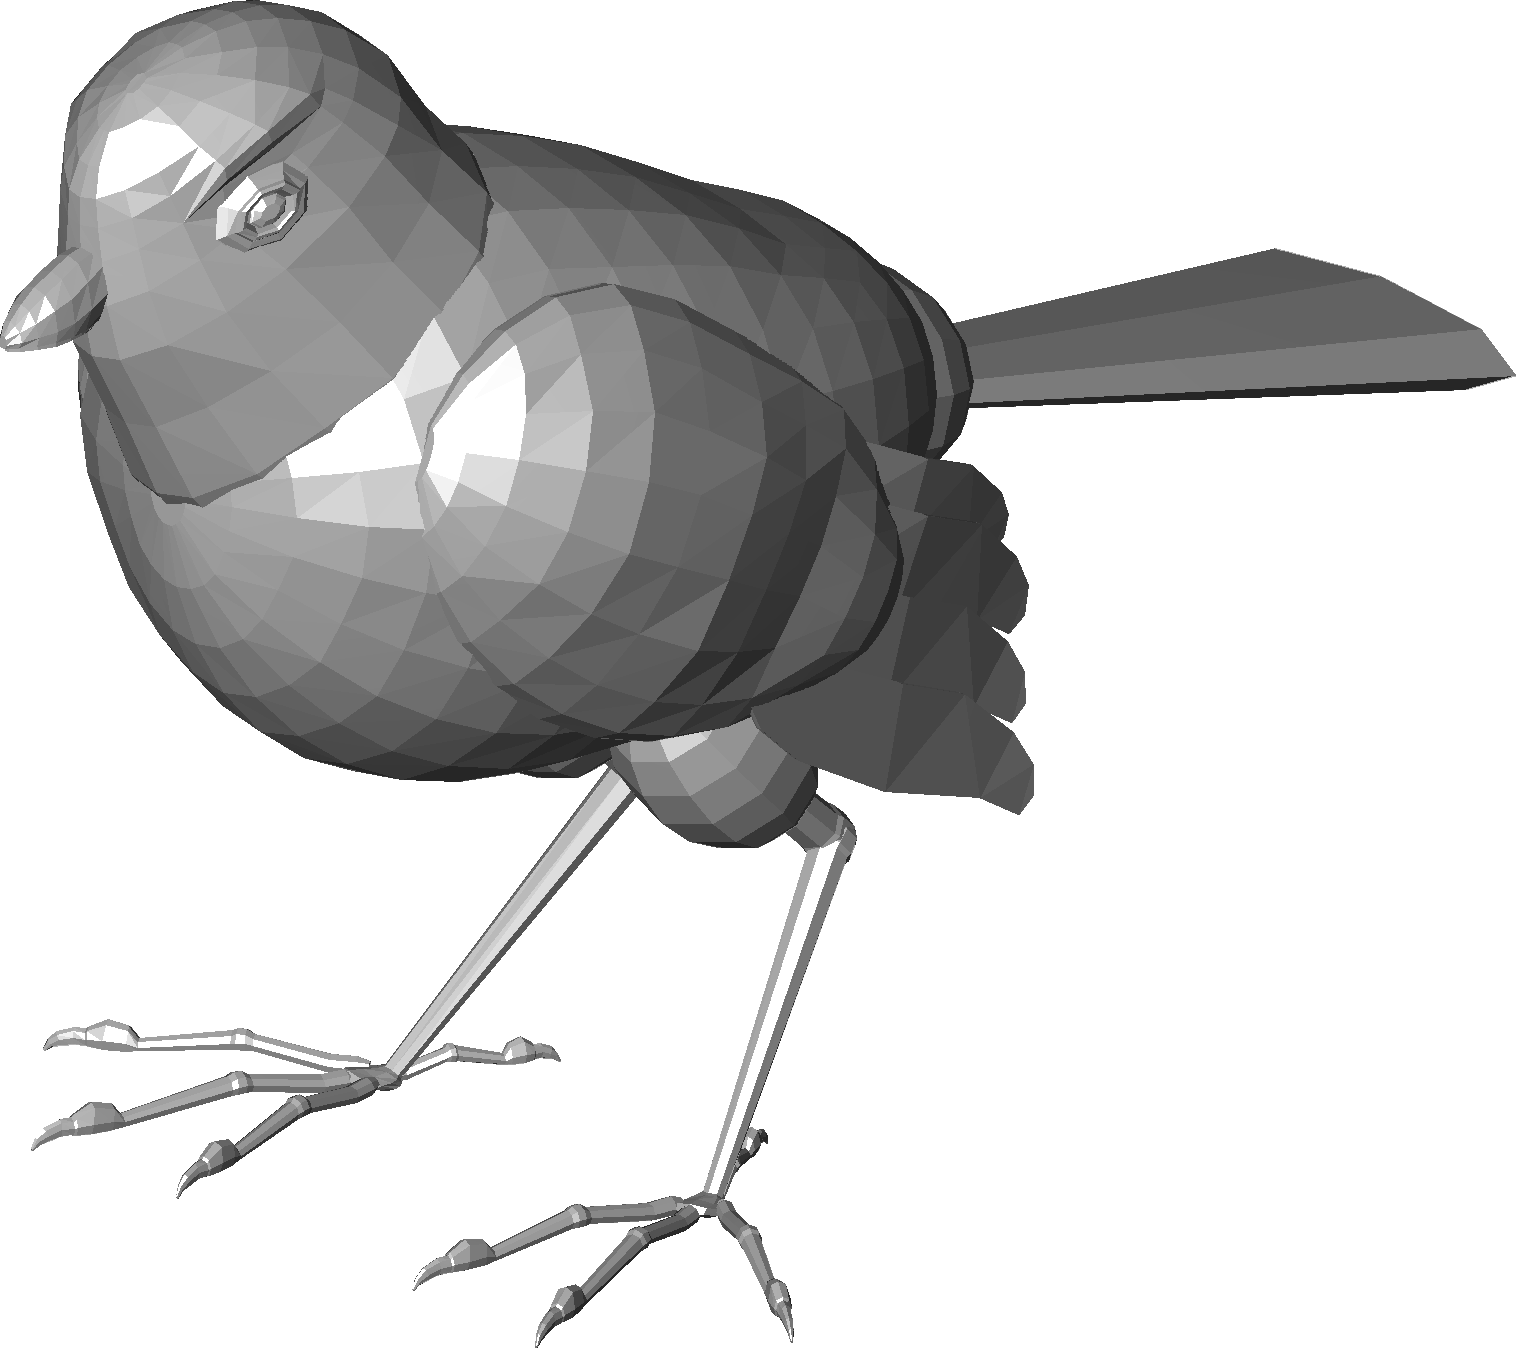
\includegraphics[width=1\linewidth]{./fig/eval/03bird.png}  
		\caption{Bird} 	
	\end{subfigure}
	\begin{subfigure}[t]{0.19\linewidth} \centering
		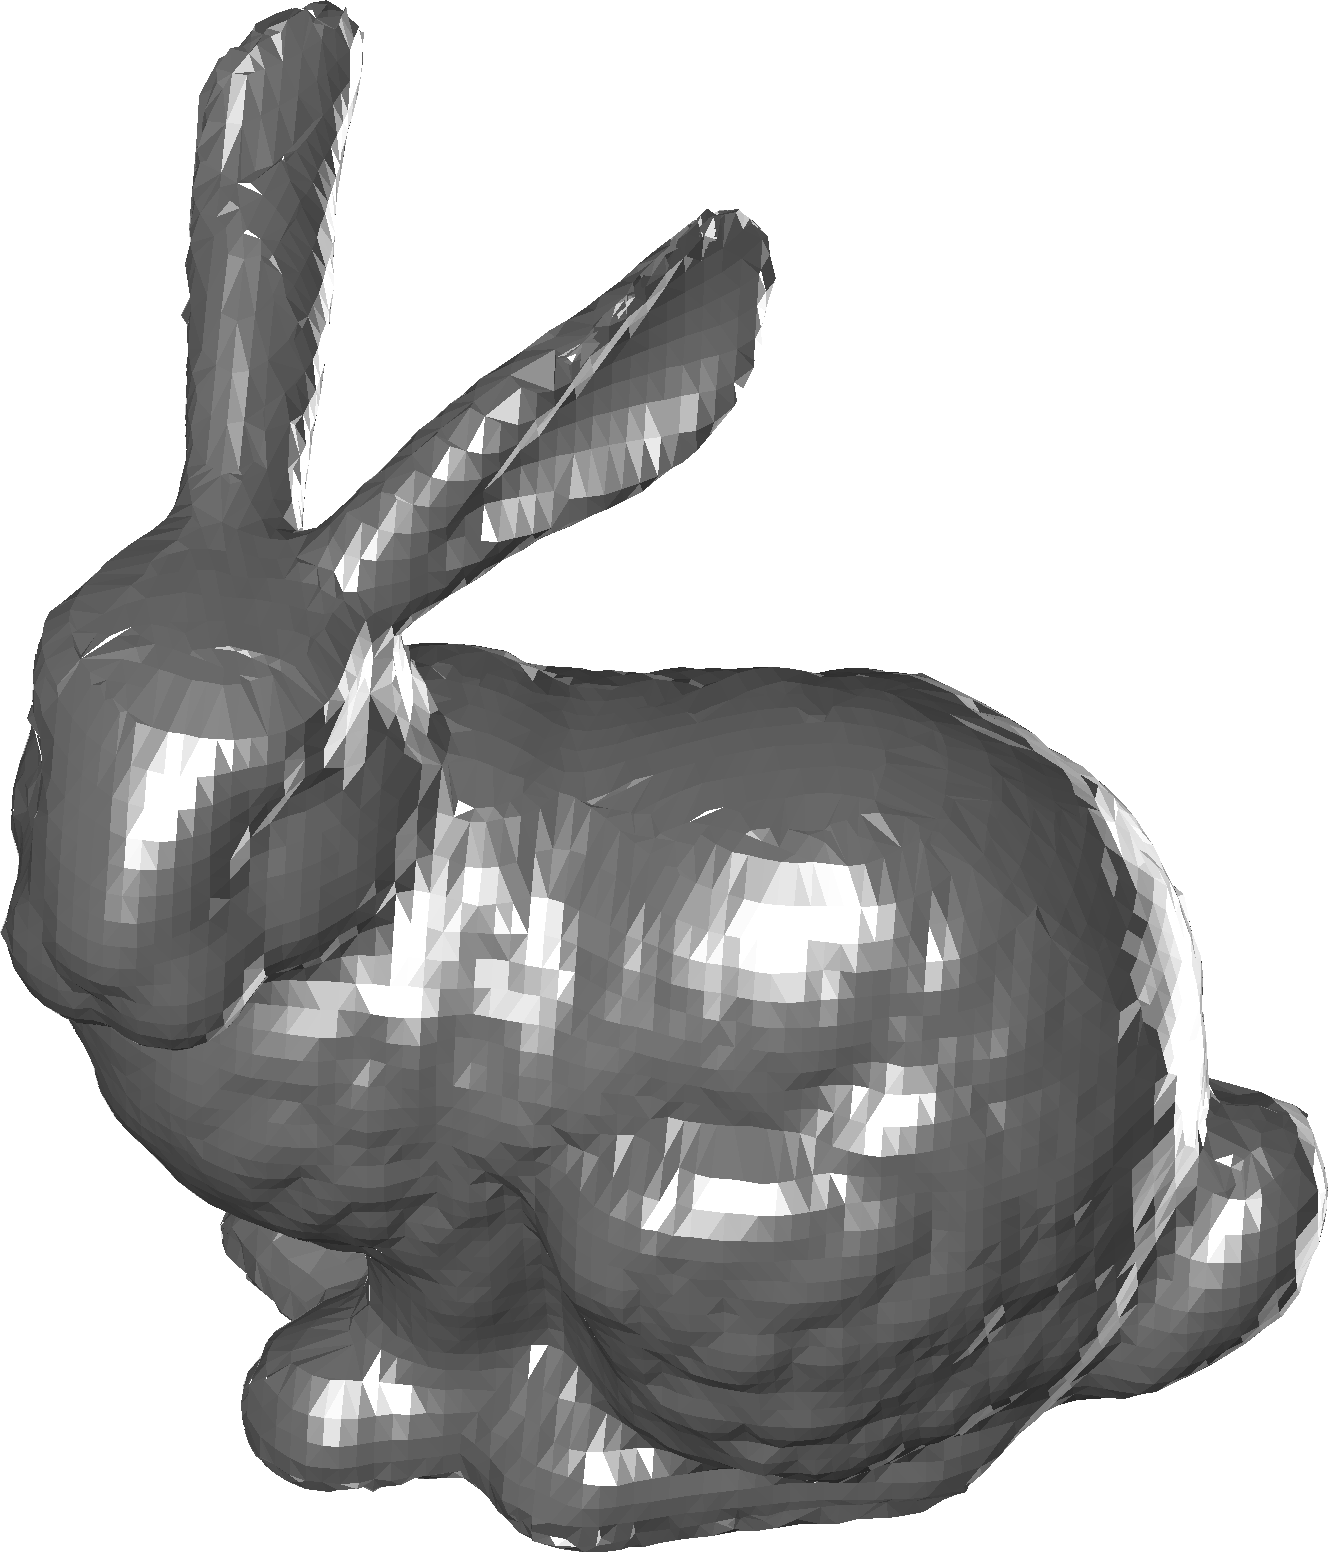
\includegraphics[width=0.9\linewidth]{./fig/eval/04bunny.png}  
		\caption{Bunny} 	
	\end{subfigure} 
	\begin{subfigure}[t]{0.19\linewidth} \centering
		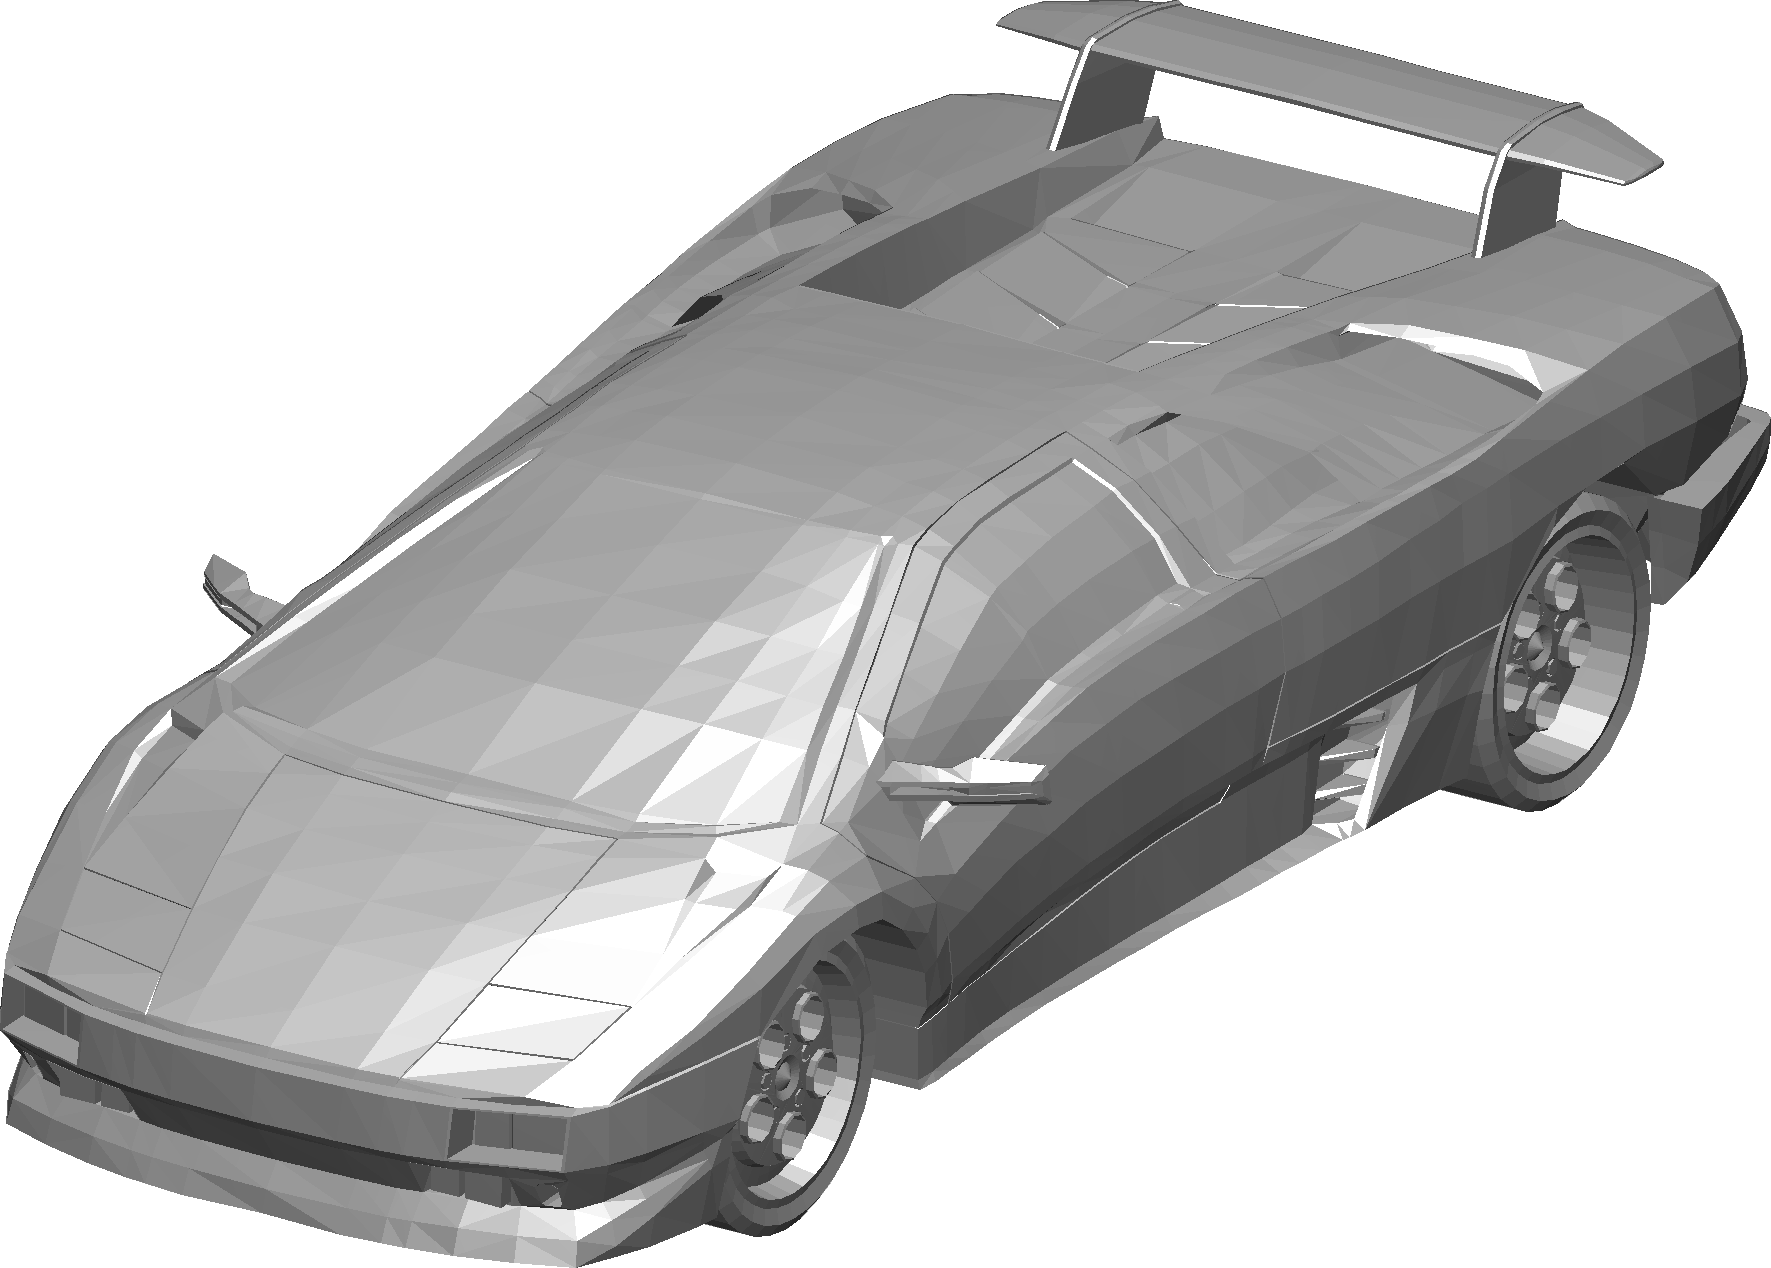
\includegraphics[width=1\linewidth]{./fig/eval/05car.png}  
		\caption{Car} 	
	\end{subfigure} \\ 
	\begin{subfigure}[t]{0.19\linewidth} \centering
		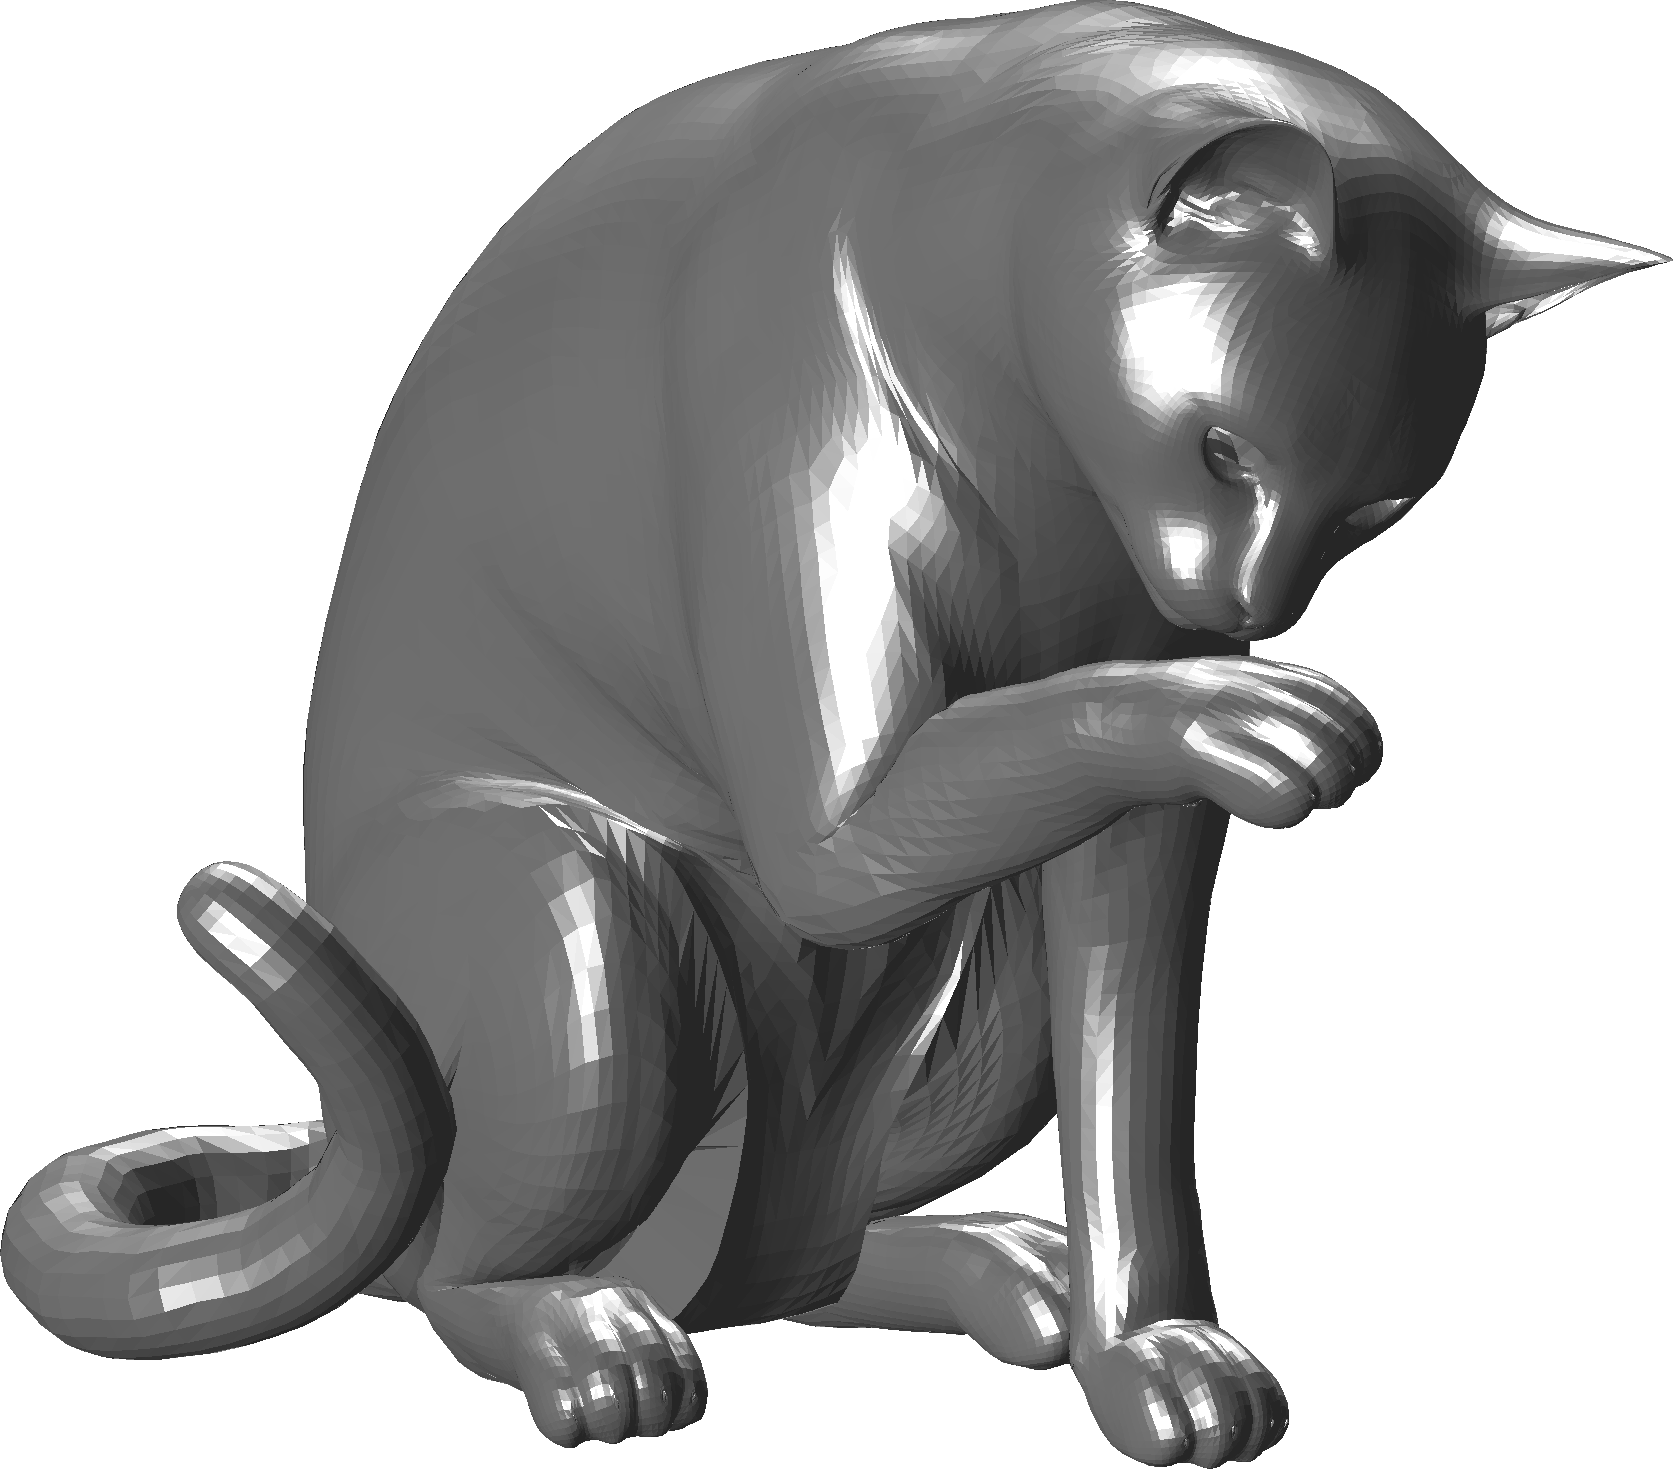
\includegraphics[width=1\linewidth]{./fig/eval/06cat.png}  
		\caption{Cat} 	
	\end{subfigure}
	\begin{subfigure}[t]{0.19\linewidth} \centering
		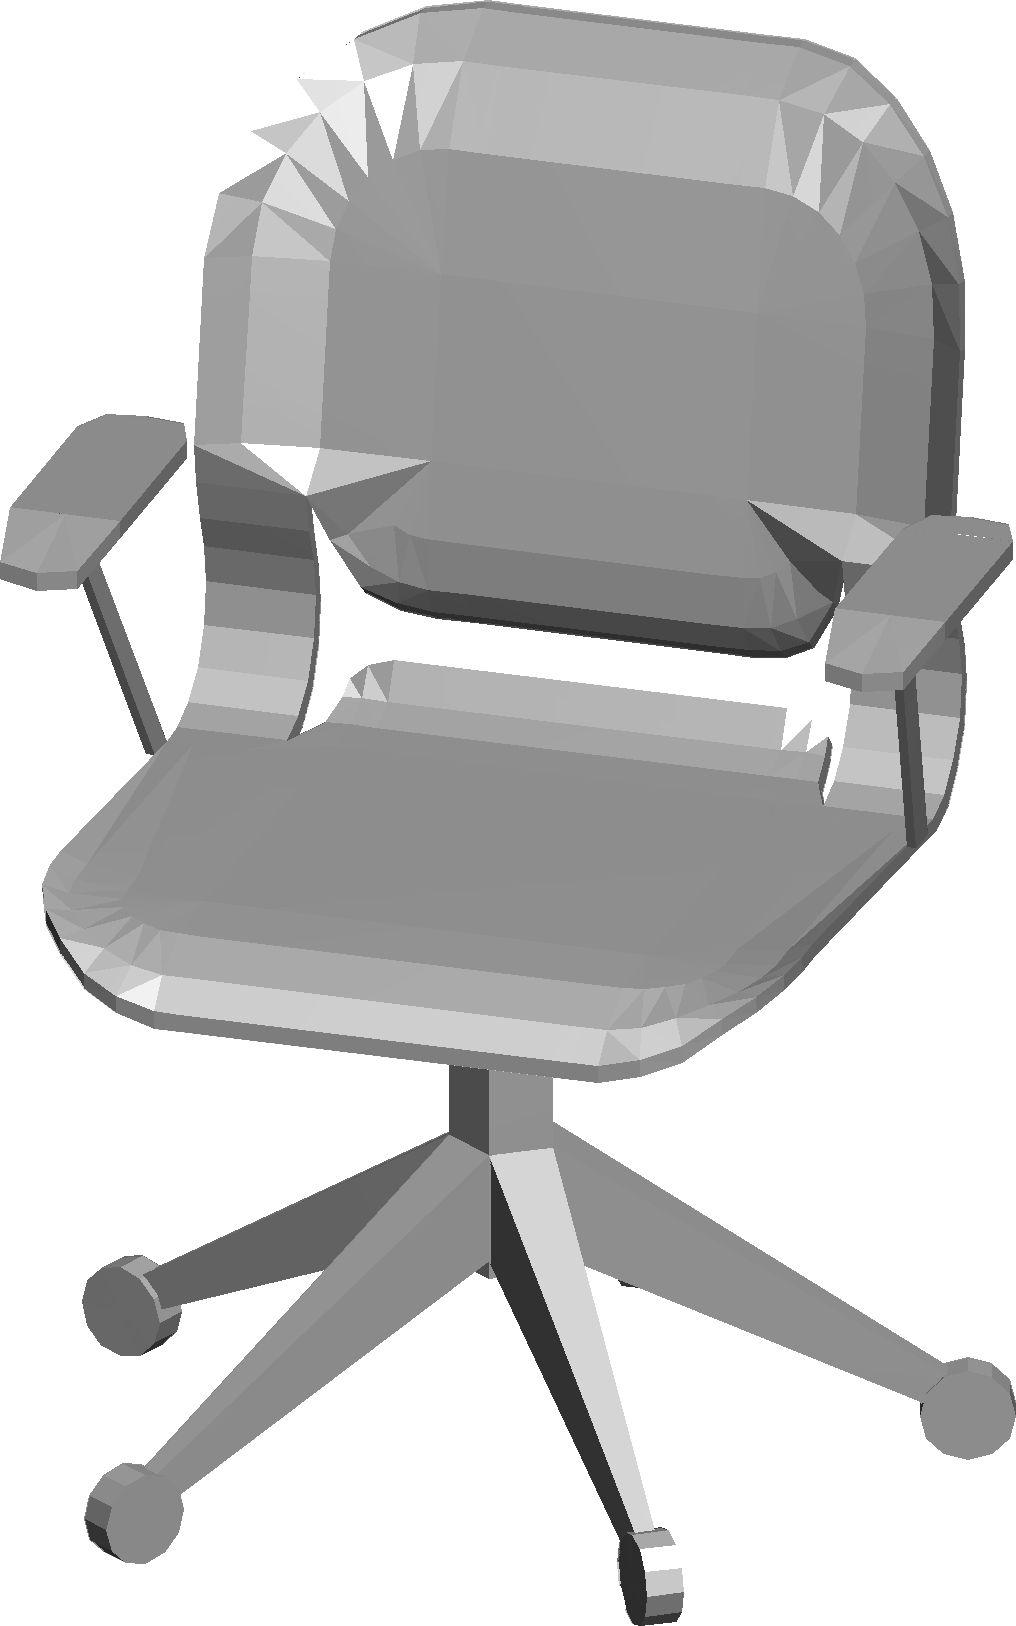
\includegraphics[width=0.7\linewidth]{./fig/eval/07chair.png}  
		\caption{Chair} 	
	\end{subfigure}
	\begin{subfigure}[t]{0.19\linewidth} \centering
		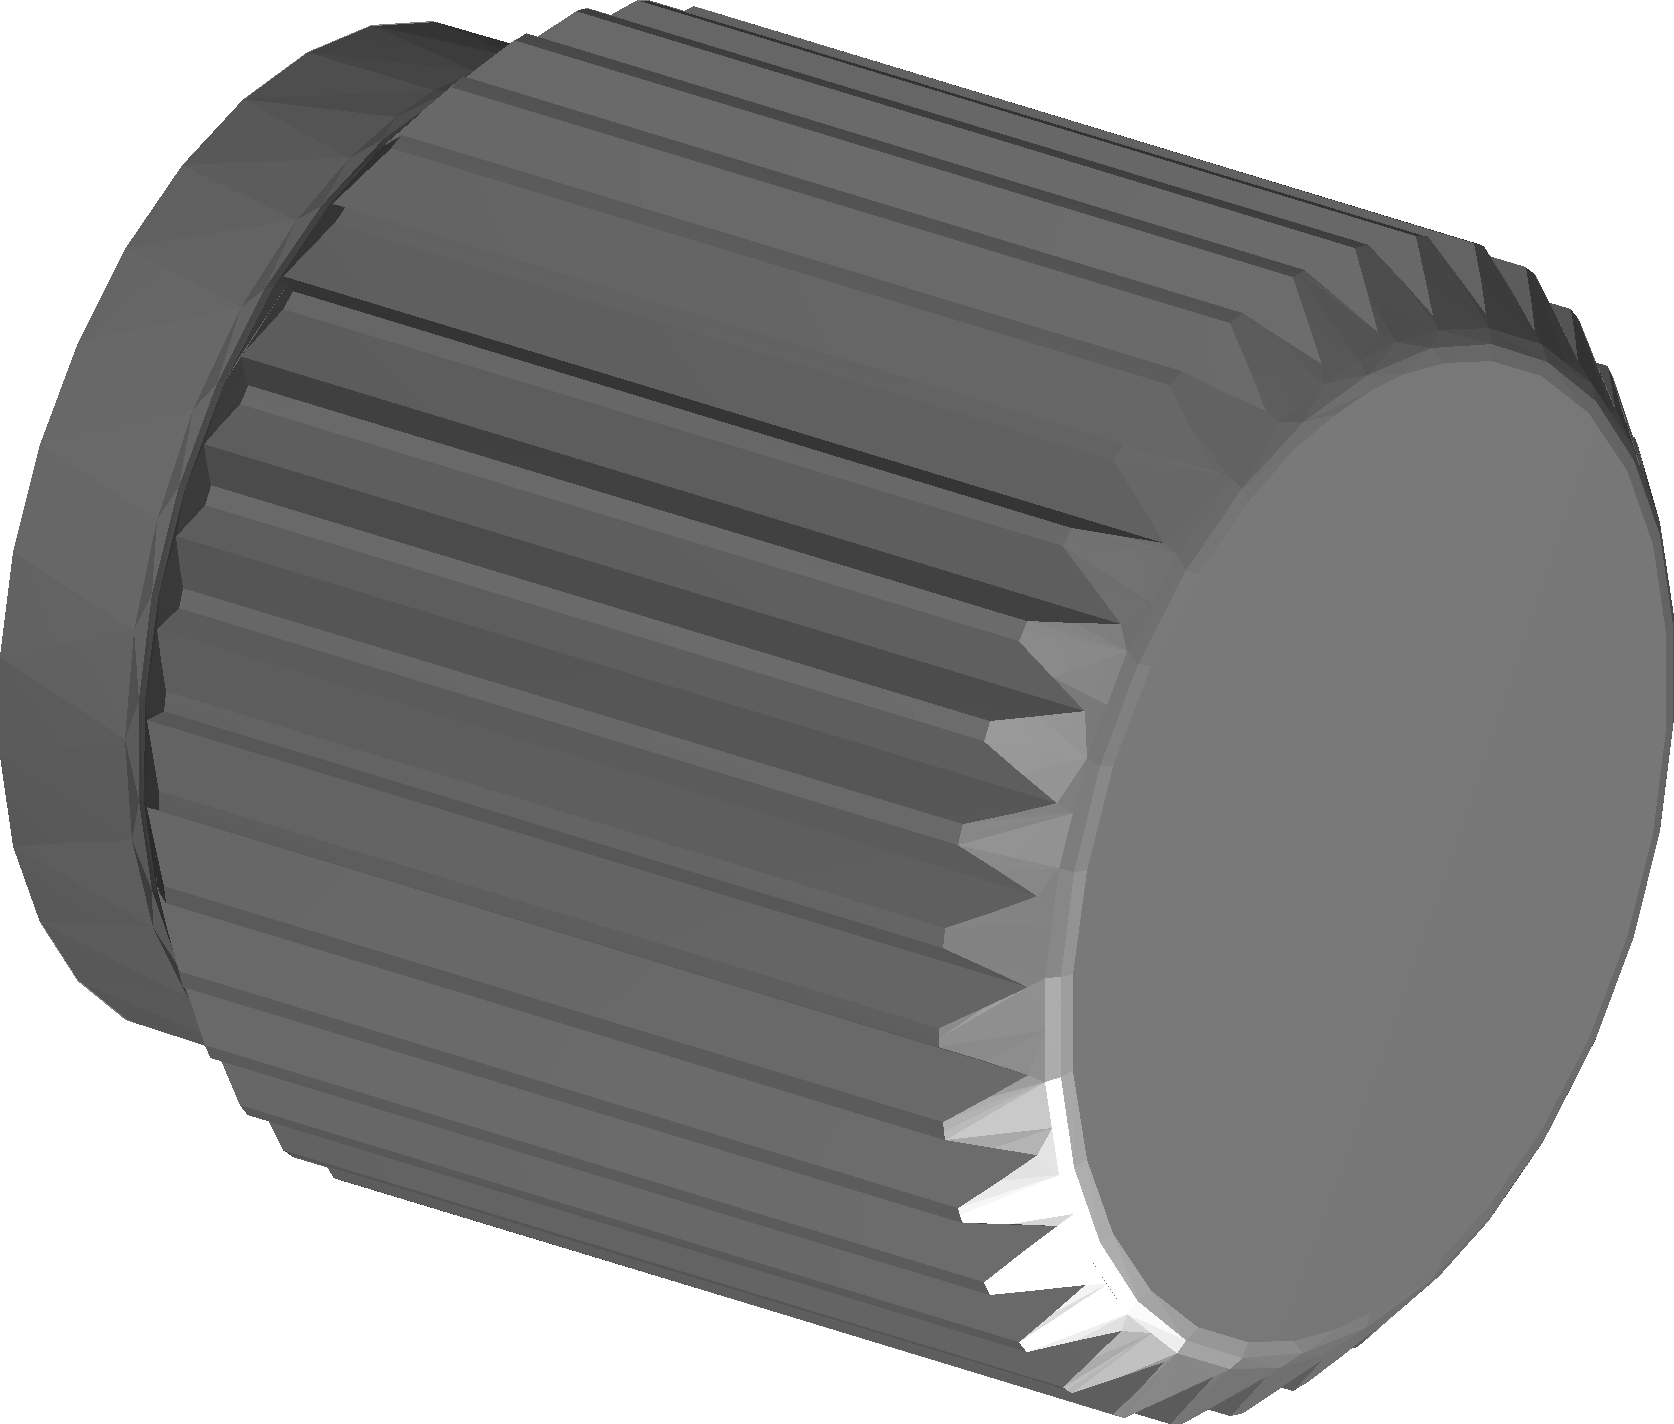
\includegraphics[width=1\linewidth]{./fig/eval/08cog.png}  
		\caption{Cog} 	
	\end{subfigure}
	\begin{subfigure}[t]{0.19\linewidth} \centering
		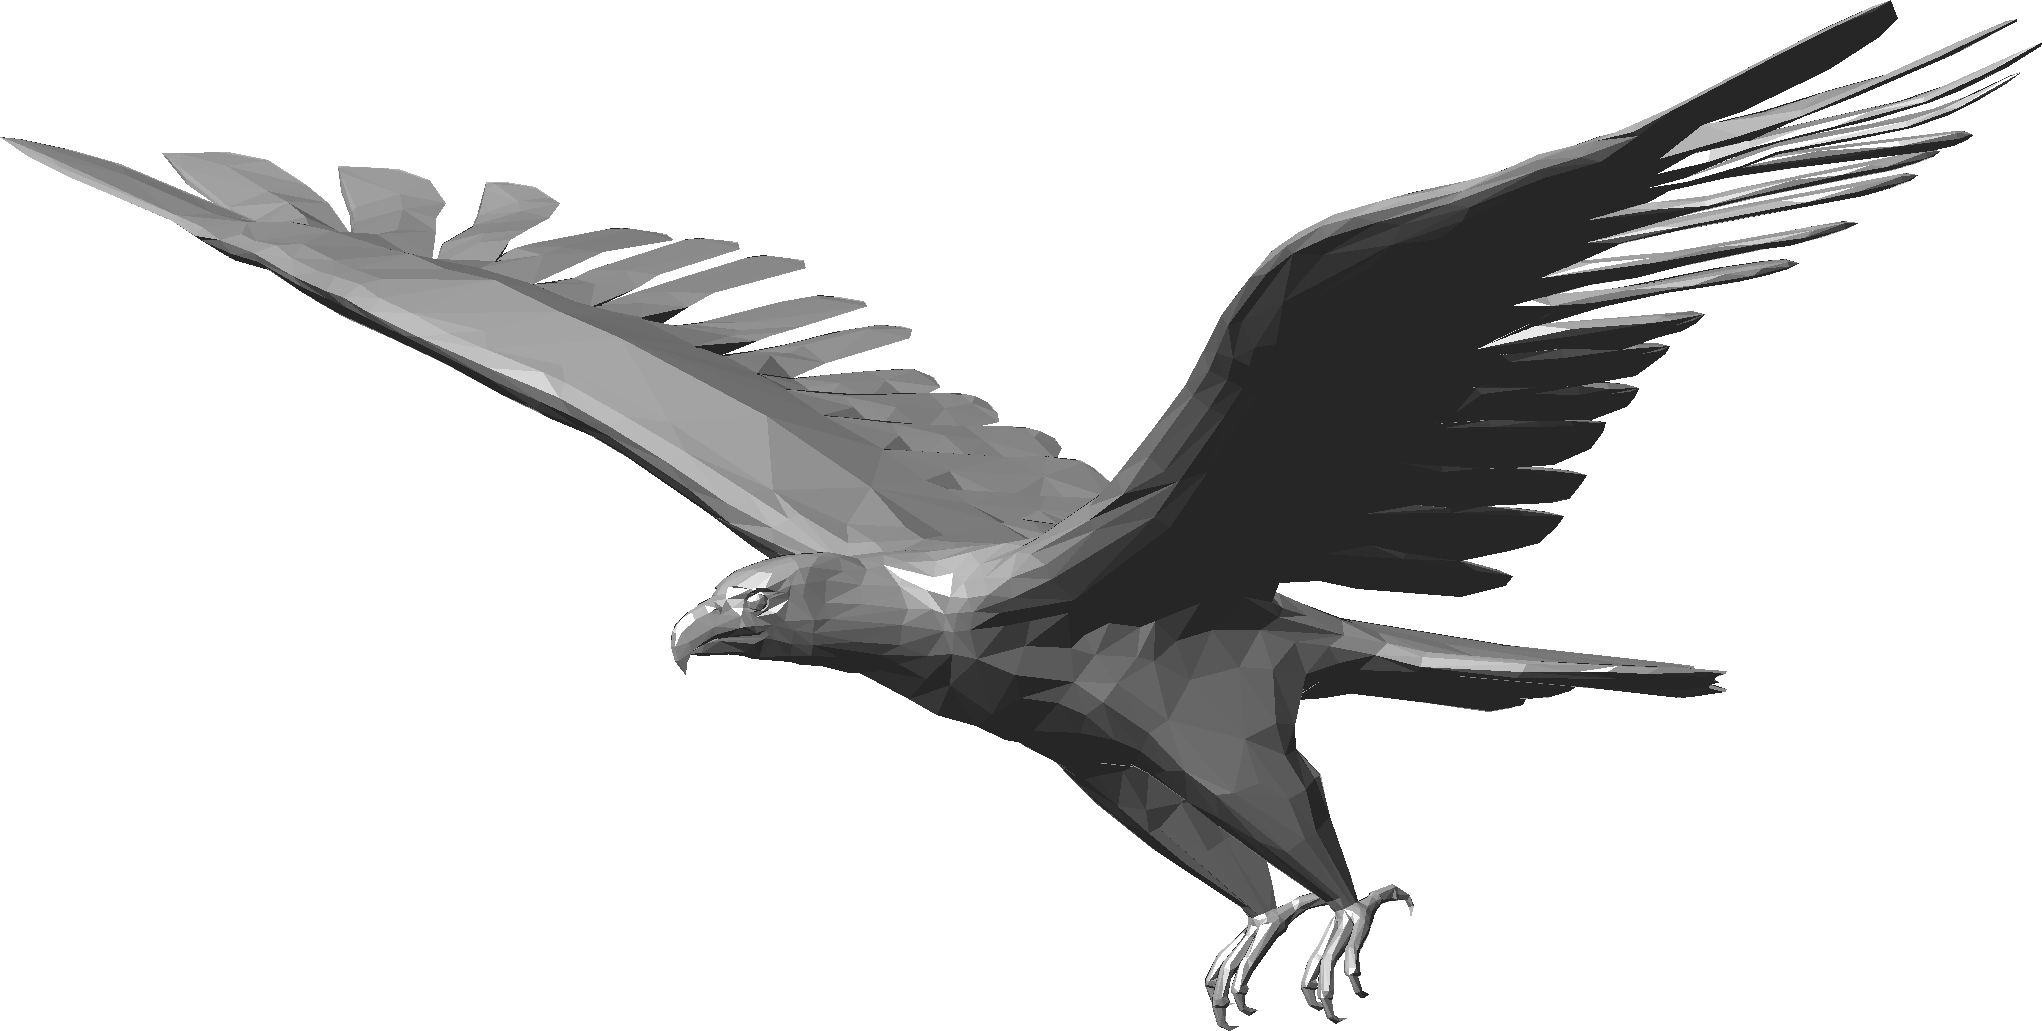
\includegraphics[width=1\linewidth]{./fig/eval/09eagle.png}  
		\caption{Eagle} 	
	\end{subfigure} 
	\begin{subfigure}[t]{0.19\linewidth} \centering
		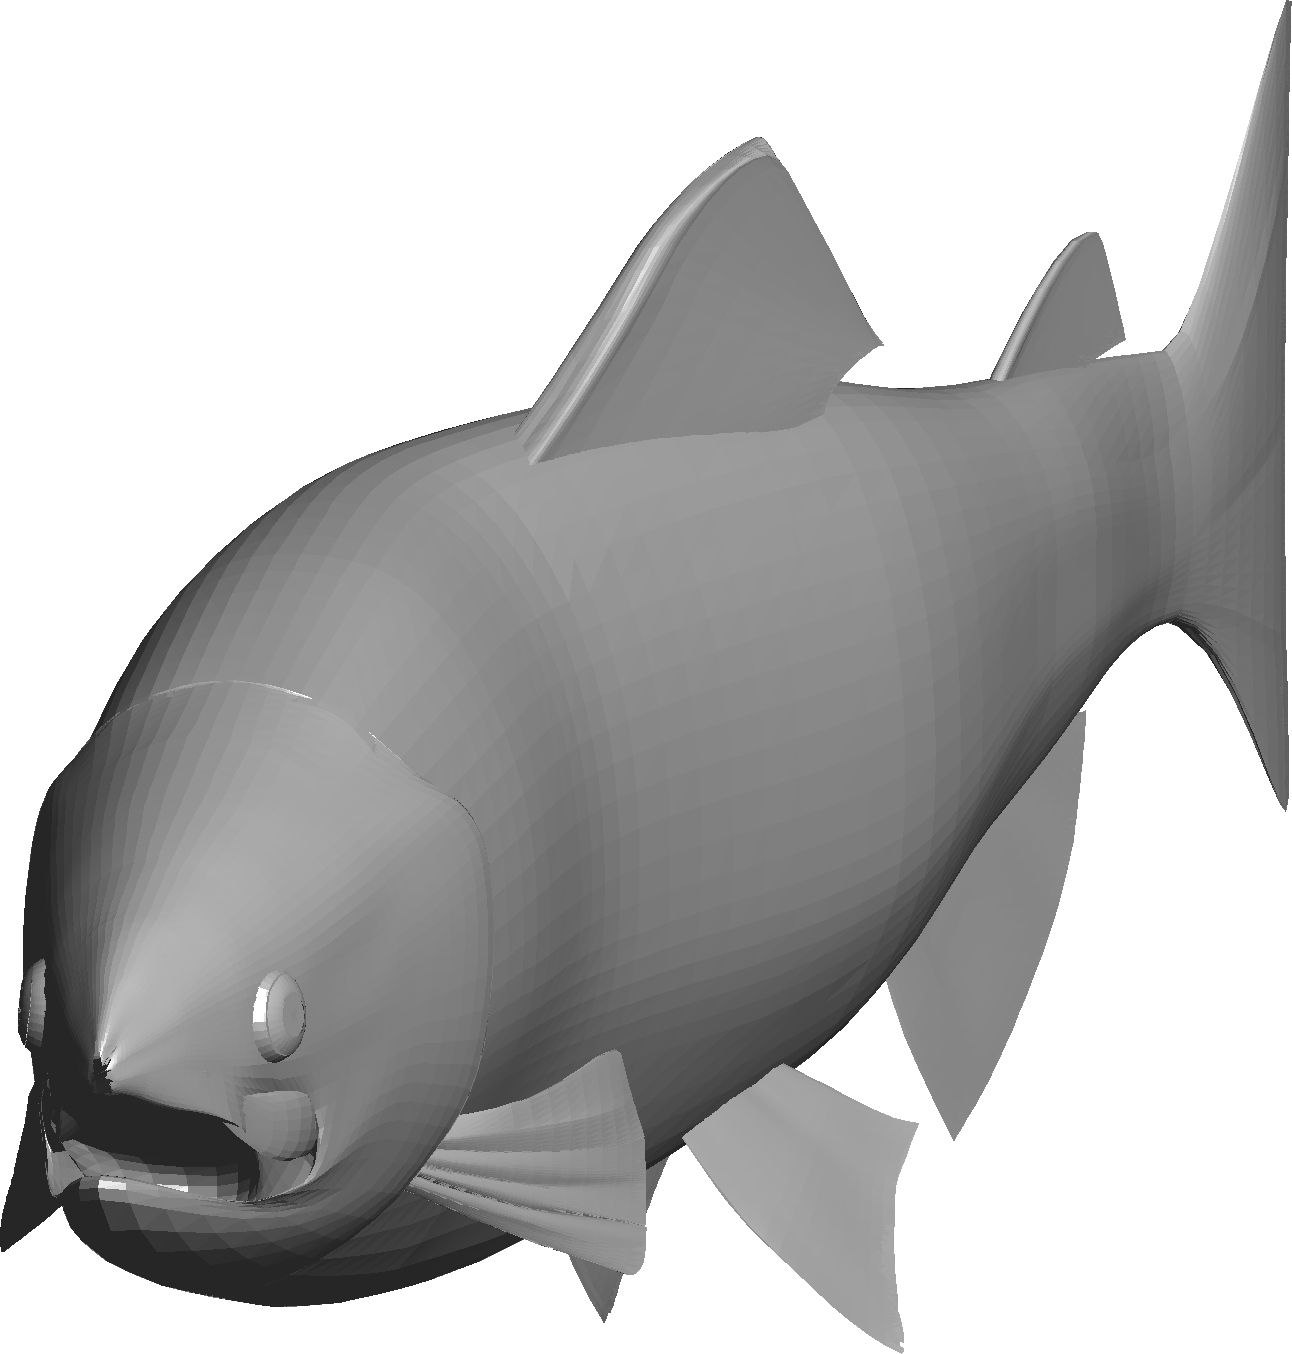
\includegraphics[width=1\linewidth]{./fig/eval/10fish.png}  
		\caption{Fish} 	
	\end{subfigure} \\ 
	\begin{subfigure}[t]{0.19\linewidth} \centering
		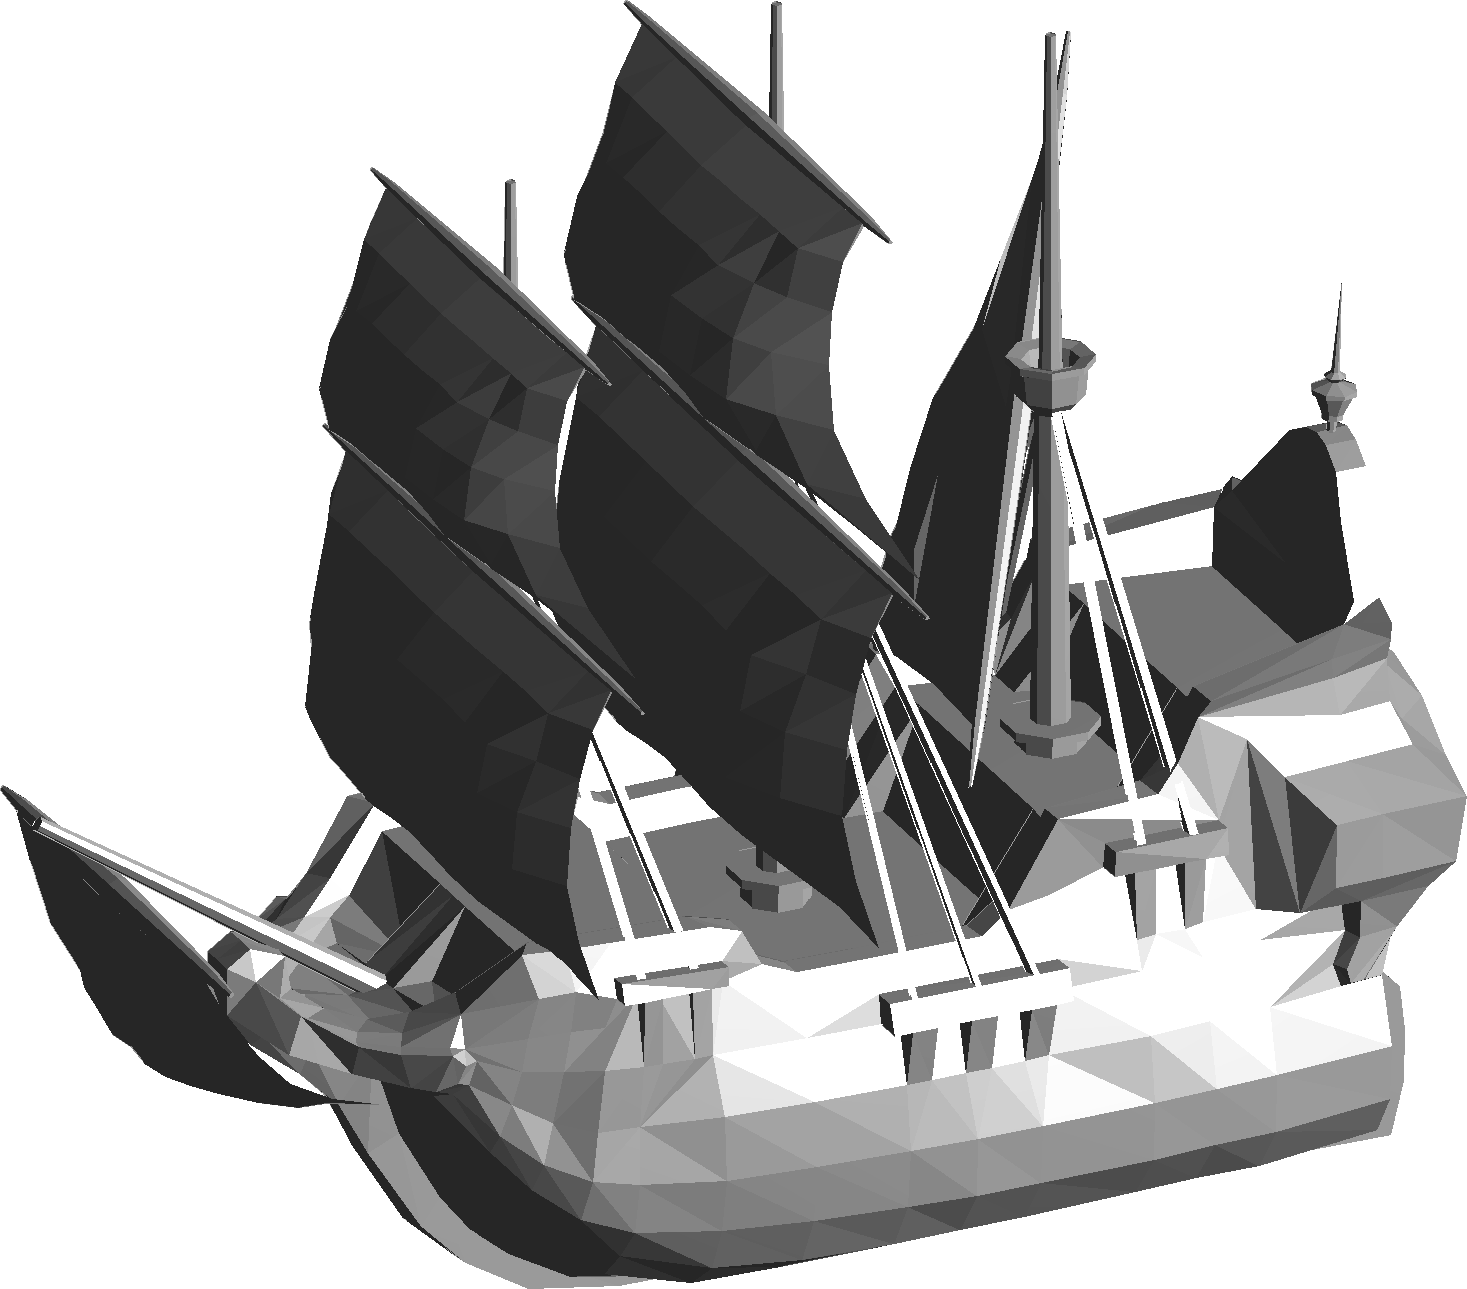
\includegraphics[width=1\linewidth]{./fig/eval/11galleon.png}  
		\caption{Galleon} 	
	\end{subfigure}
	\begin{subfigure}[t]{0.19\linewidth} \centering
		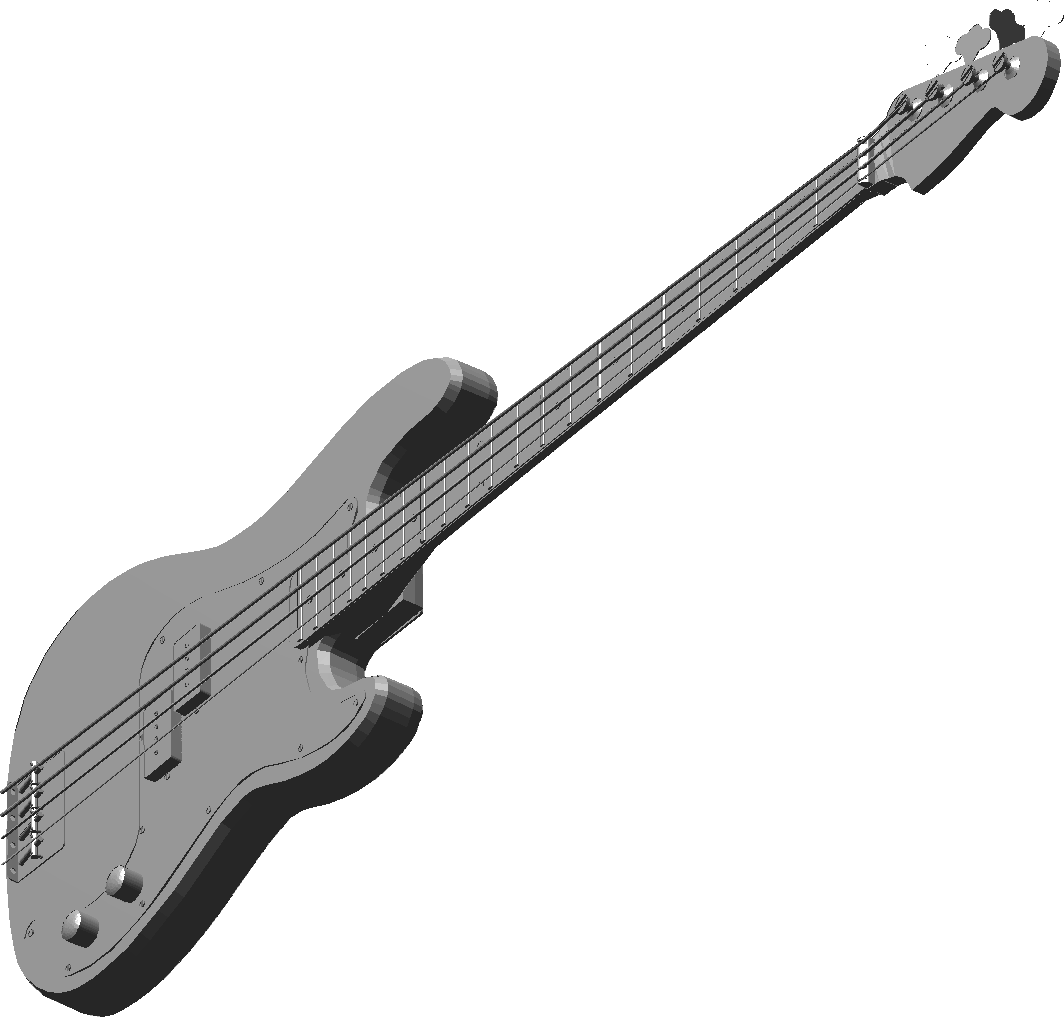
\includegraphics[width=1\linewidth]{./fig/eval/12guitar.png}  
		\caption{Guitar} 	
	\end{subfigure}
	\begin{subfigure}[t]{0.19\linewidth} \centering
		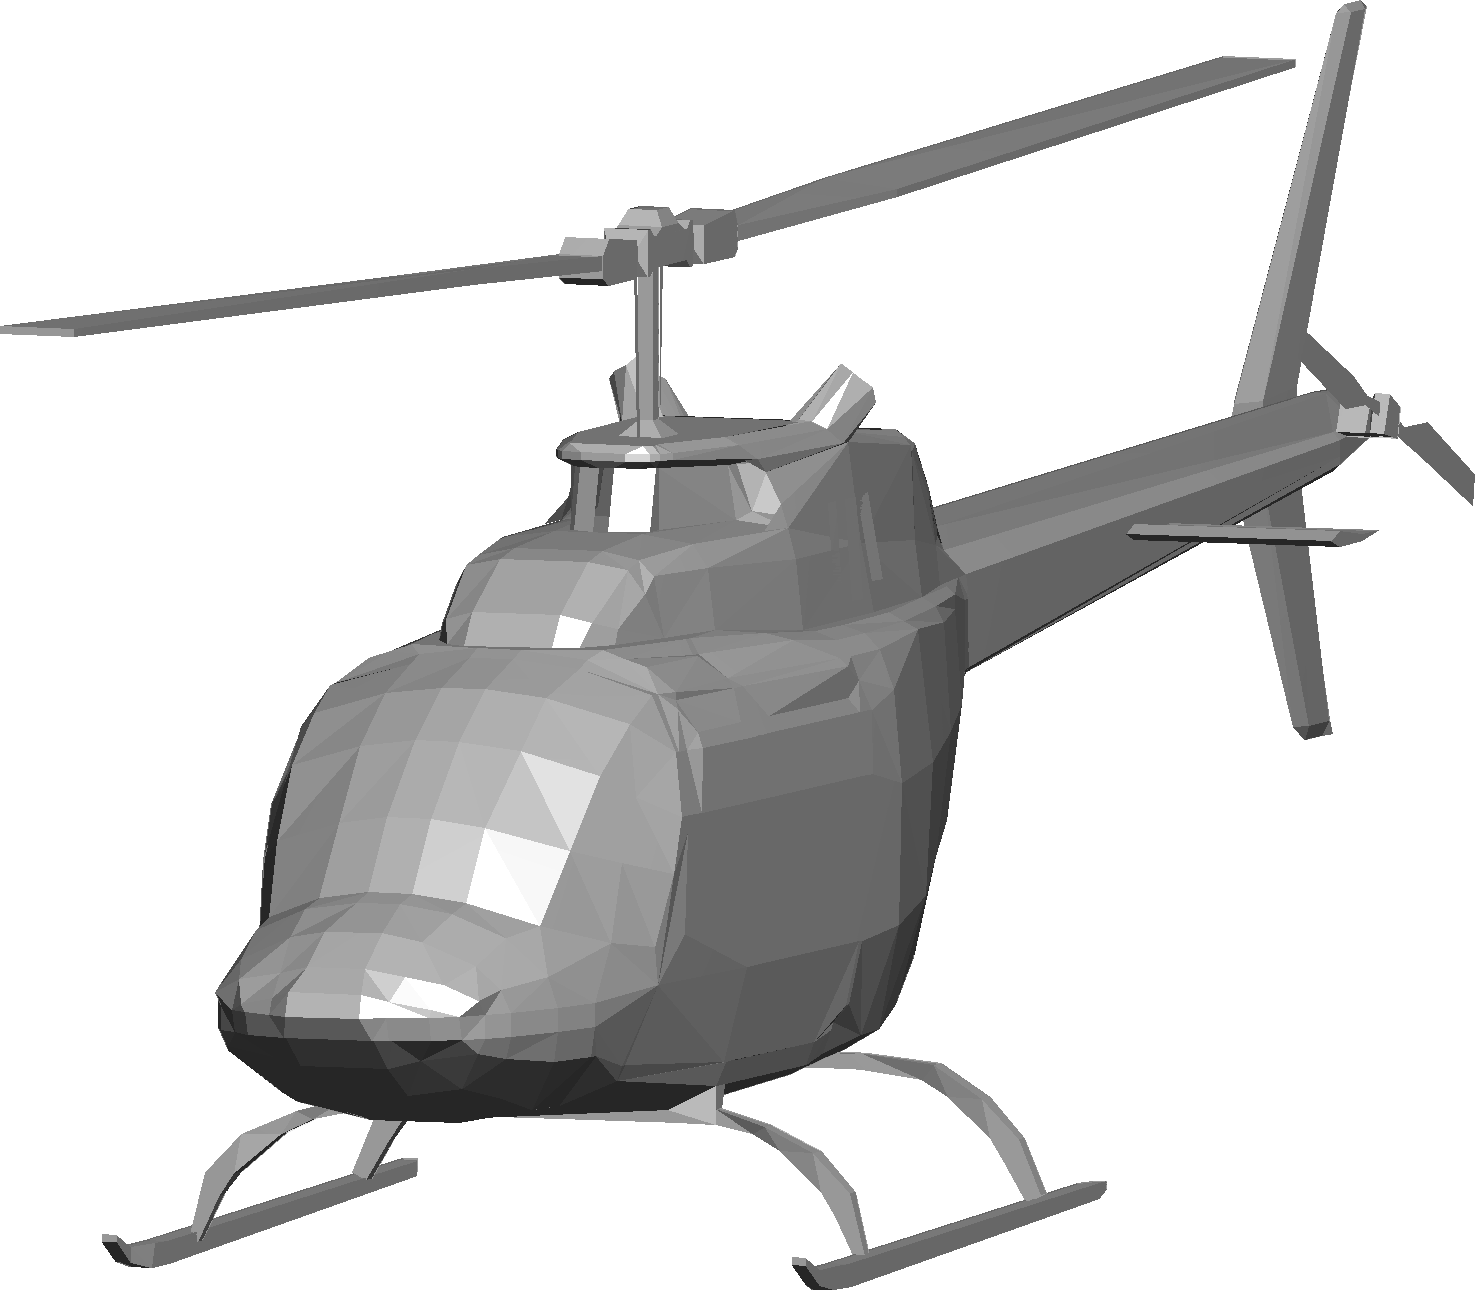
\includegraphics[width=1\linewidth]{./fig/eval/13helicopter.png}  
		\caption{Helicopter} 	
	\end{subfigure}
	\begin{subfigure}[t]{0.19\linewidth} \centering
		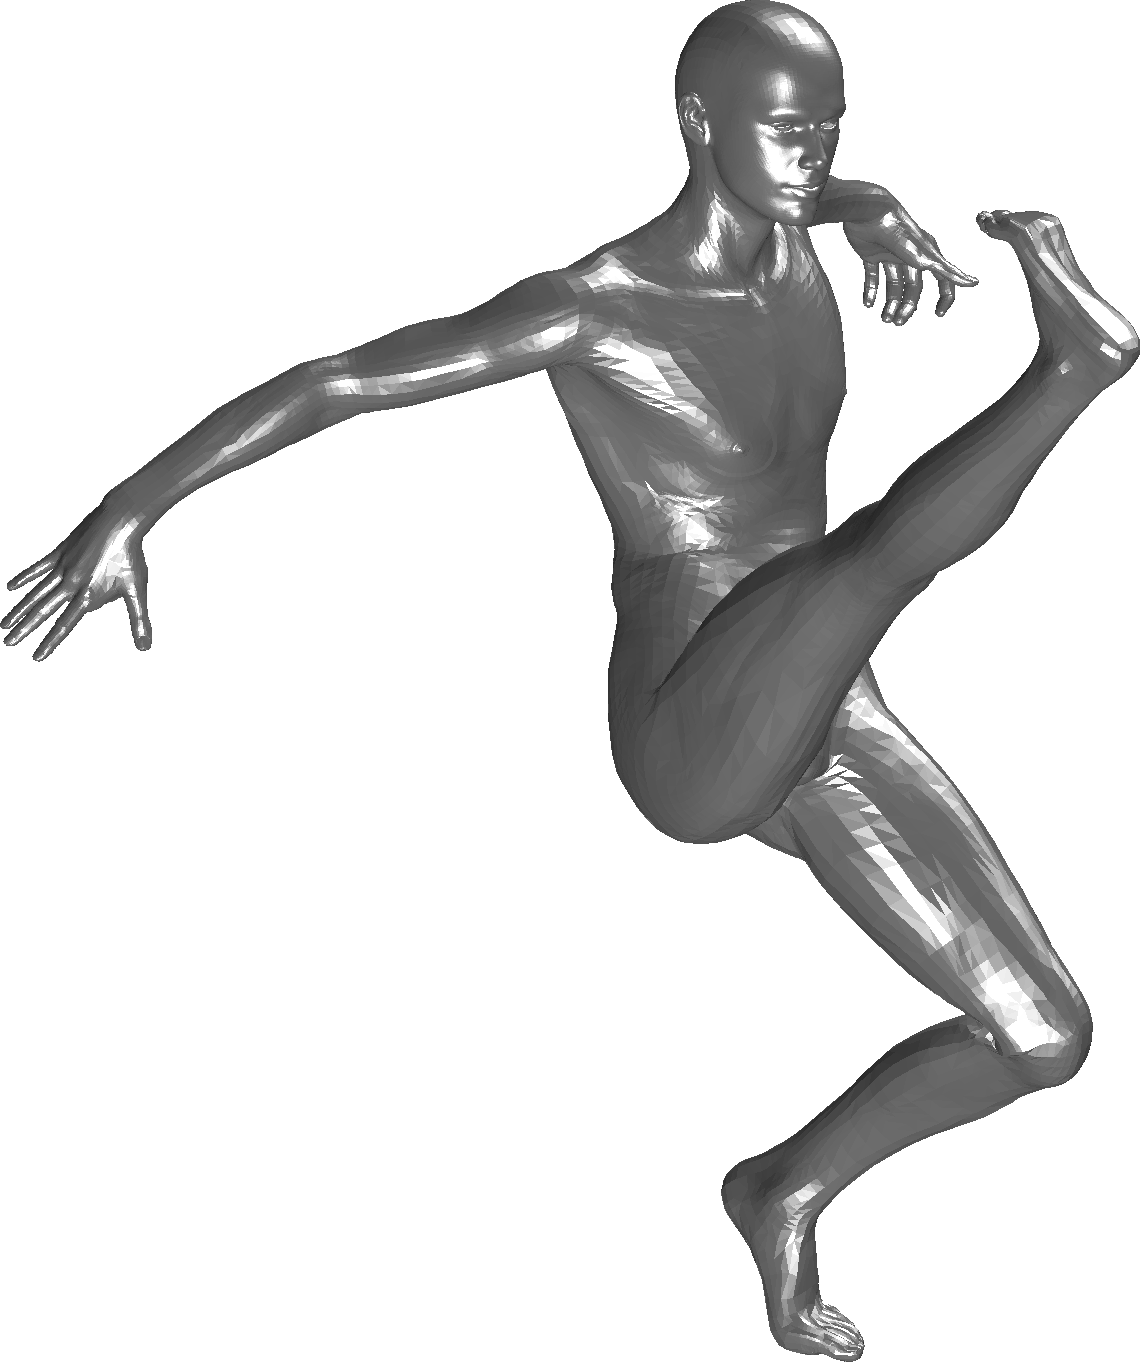
\includegraphics[width=0.8\linewidth]{./fig/eval/14man.png}  
		\caption{Kicking man} 	
	\end{subfigure} 
	\begin{subfigure}[t]{0.19\linewidth} \centering
		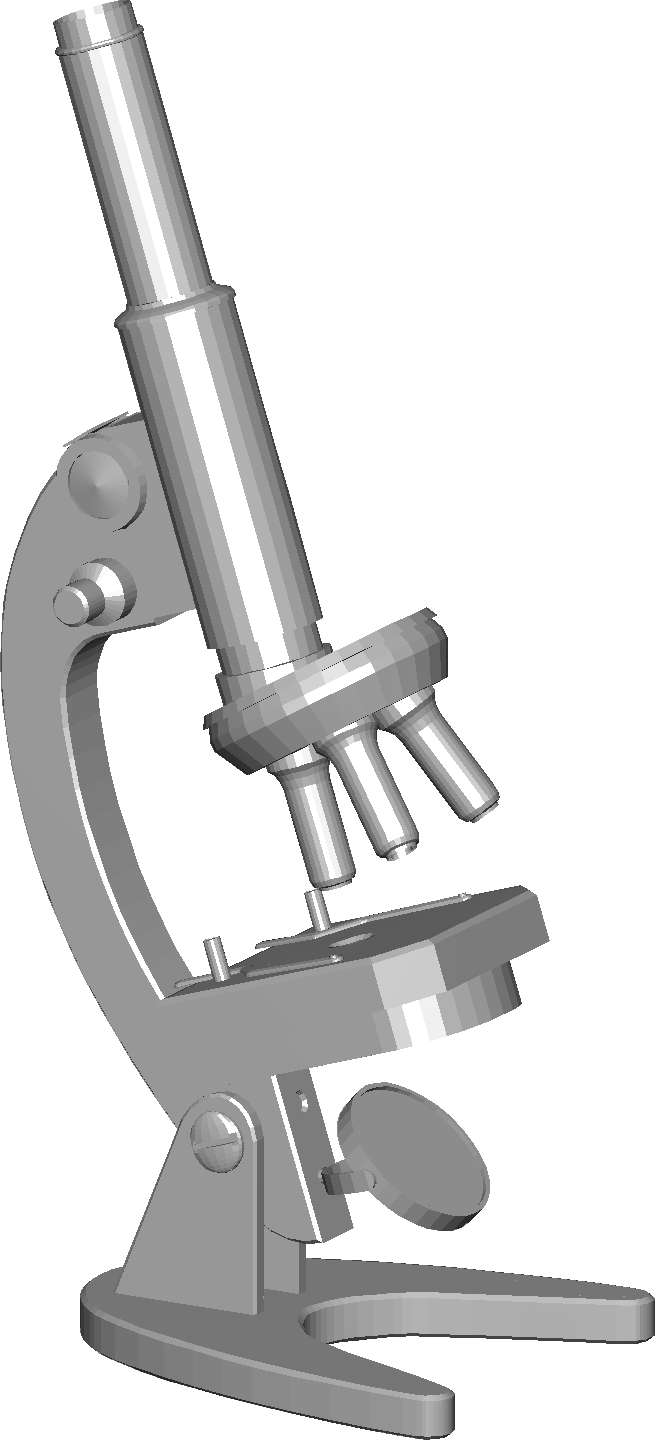
\includegraphics[width=0.5\linewidth]{./fig/eval/15microscope.png}  
		\caption{Microscope} 	
	\end{subfigure} \\ 
	\begin{subfigure}[t]{0.19\linewidth} \centering
		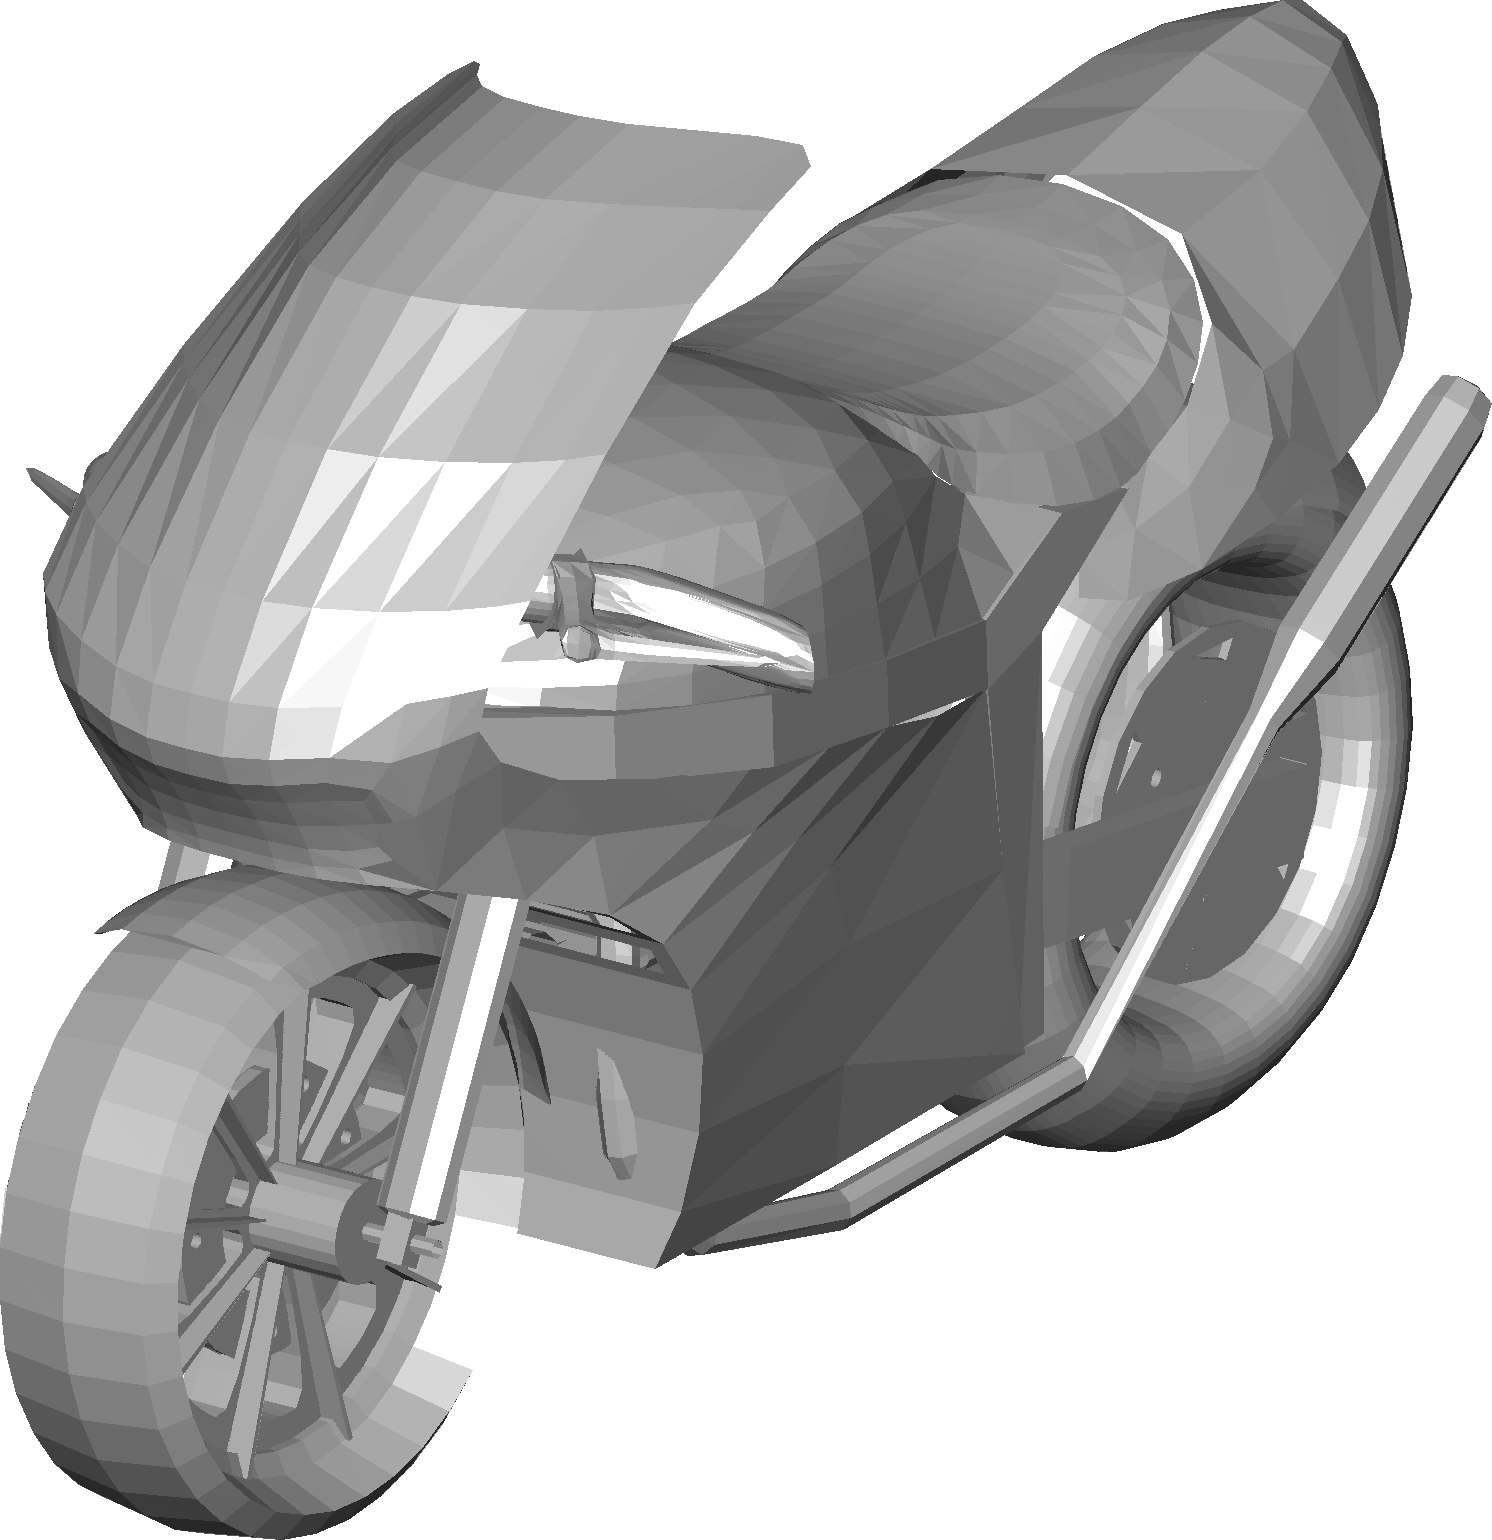
\includegraphics[width=1\linewidth]{./fig/eval/16motorbike.png}  
		\caption{Motorbike} 	
	\end{subfigure}
	\begin{subfigure}[t]{0.19\linewidth} \centering
		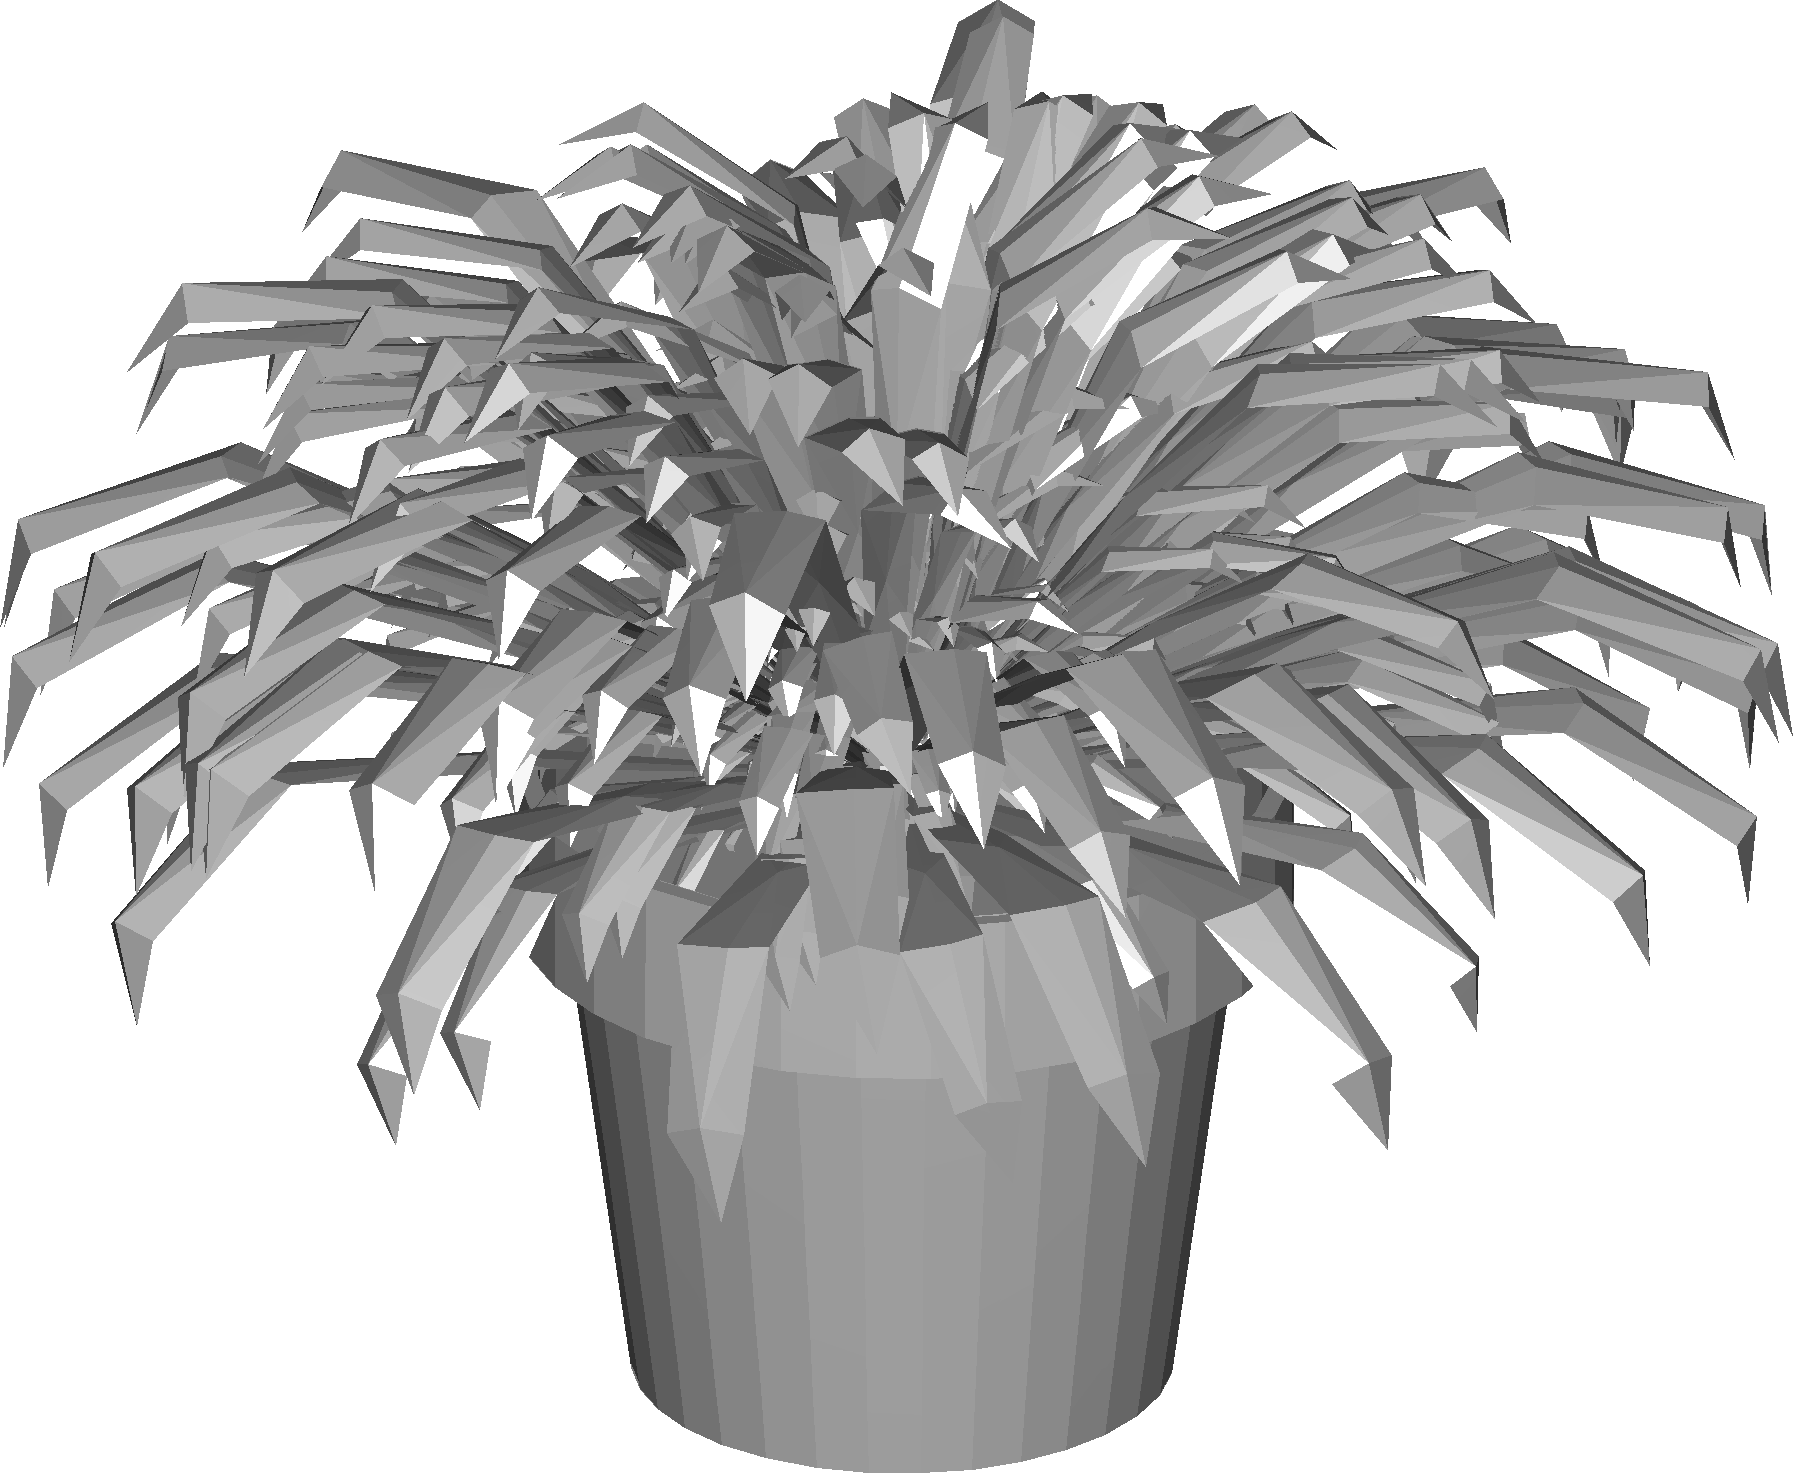
\includegraphics[width=1\linewidth]{./fig/eval/17plant.png}  
		\caption{Plant} 	
	\end{subfigure}
	\begin{subfigure}[t]{0.19\linewidth} \centering
		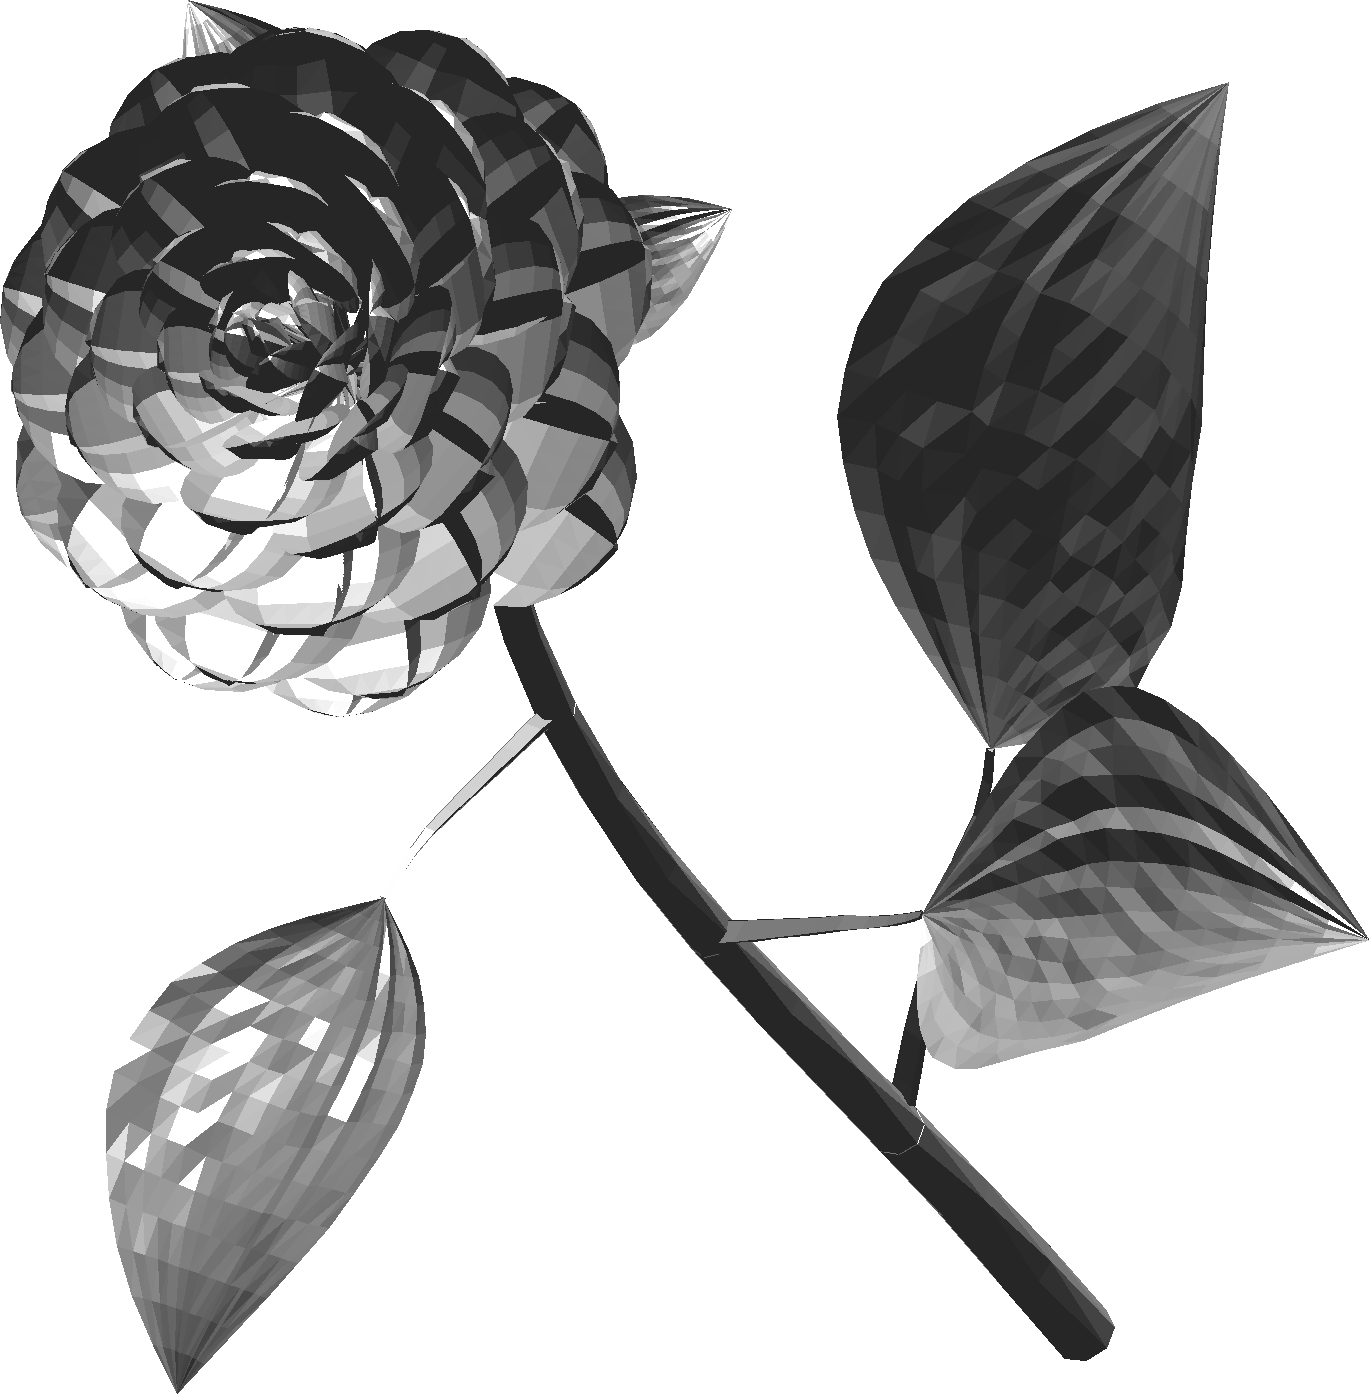
\includegraphics[width=1\linewidth]{./fig/eval/18rose.png}  
		\caption{Rose} 	
	\end{subfigure}
	\begin{subfigure}[t]{0.19\linewidth} \centering
		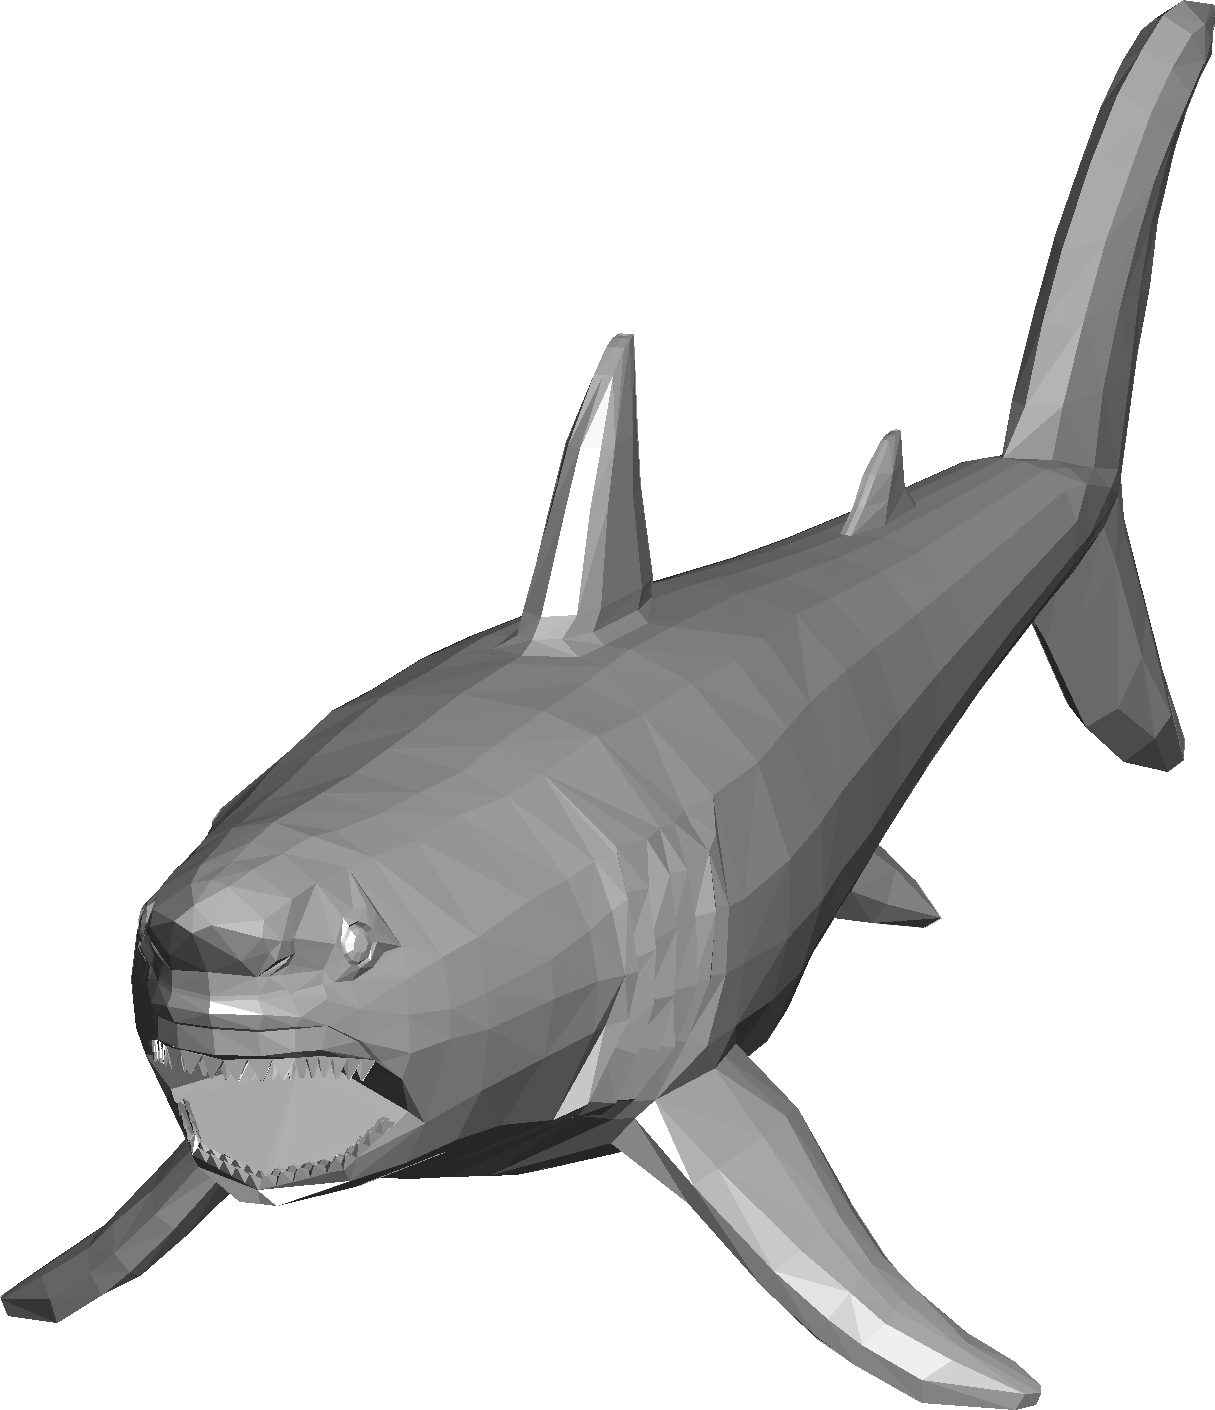
\includegraphics[width=1\linewidth]{./fig/eval/19shark.png}  
		\caption{Shark} 	
	\end{subfigure} 
	\begin{subfigure}[t]{0.19\linewidth} \centering
		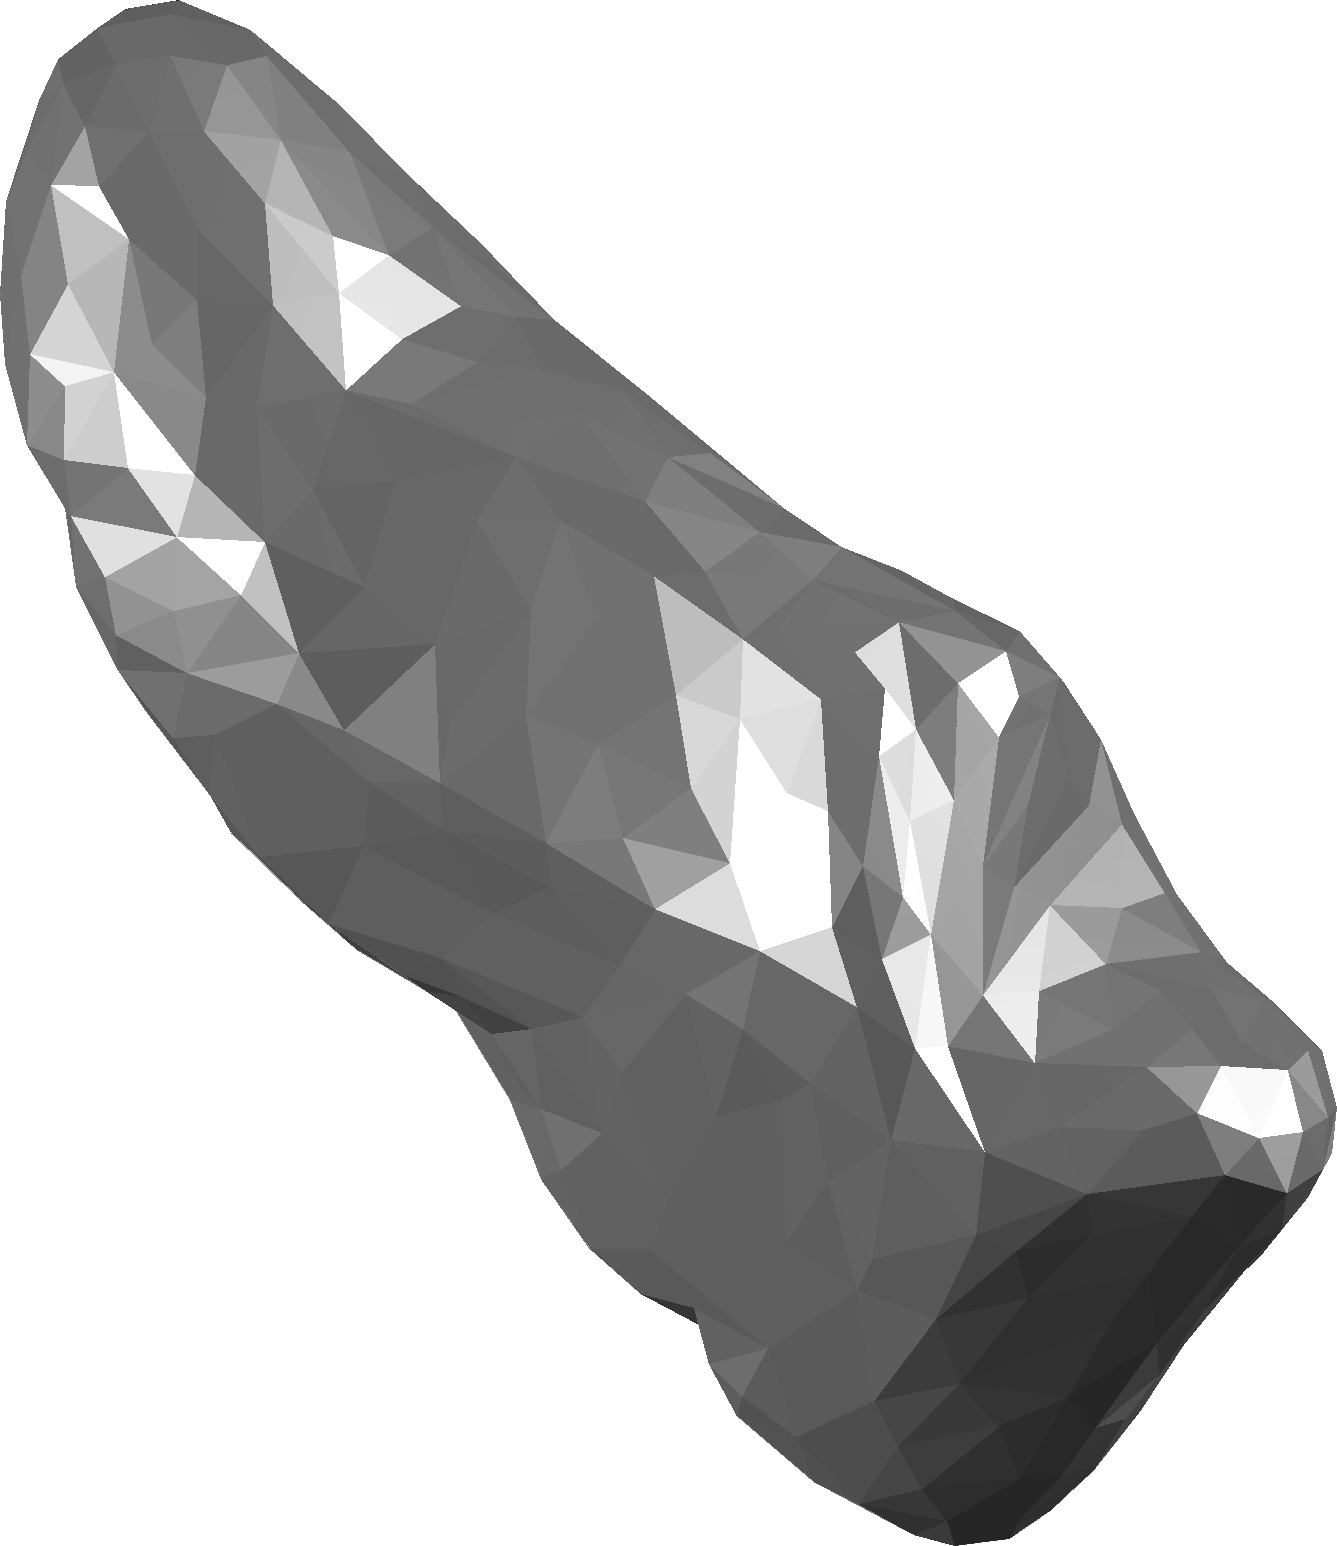
\includegraphics[width=1\linewidth]{./fig/eval/20shoe.png}  
		\caption{Shoe} 	
	\end{subfigure} \\ 
	\begin{subfigure}[t]{0.19\linewidth} \centering
		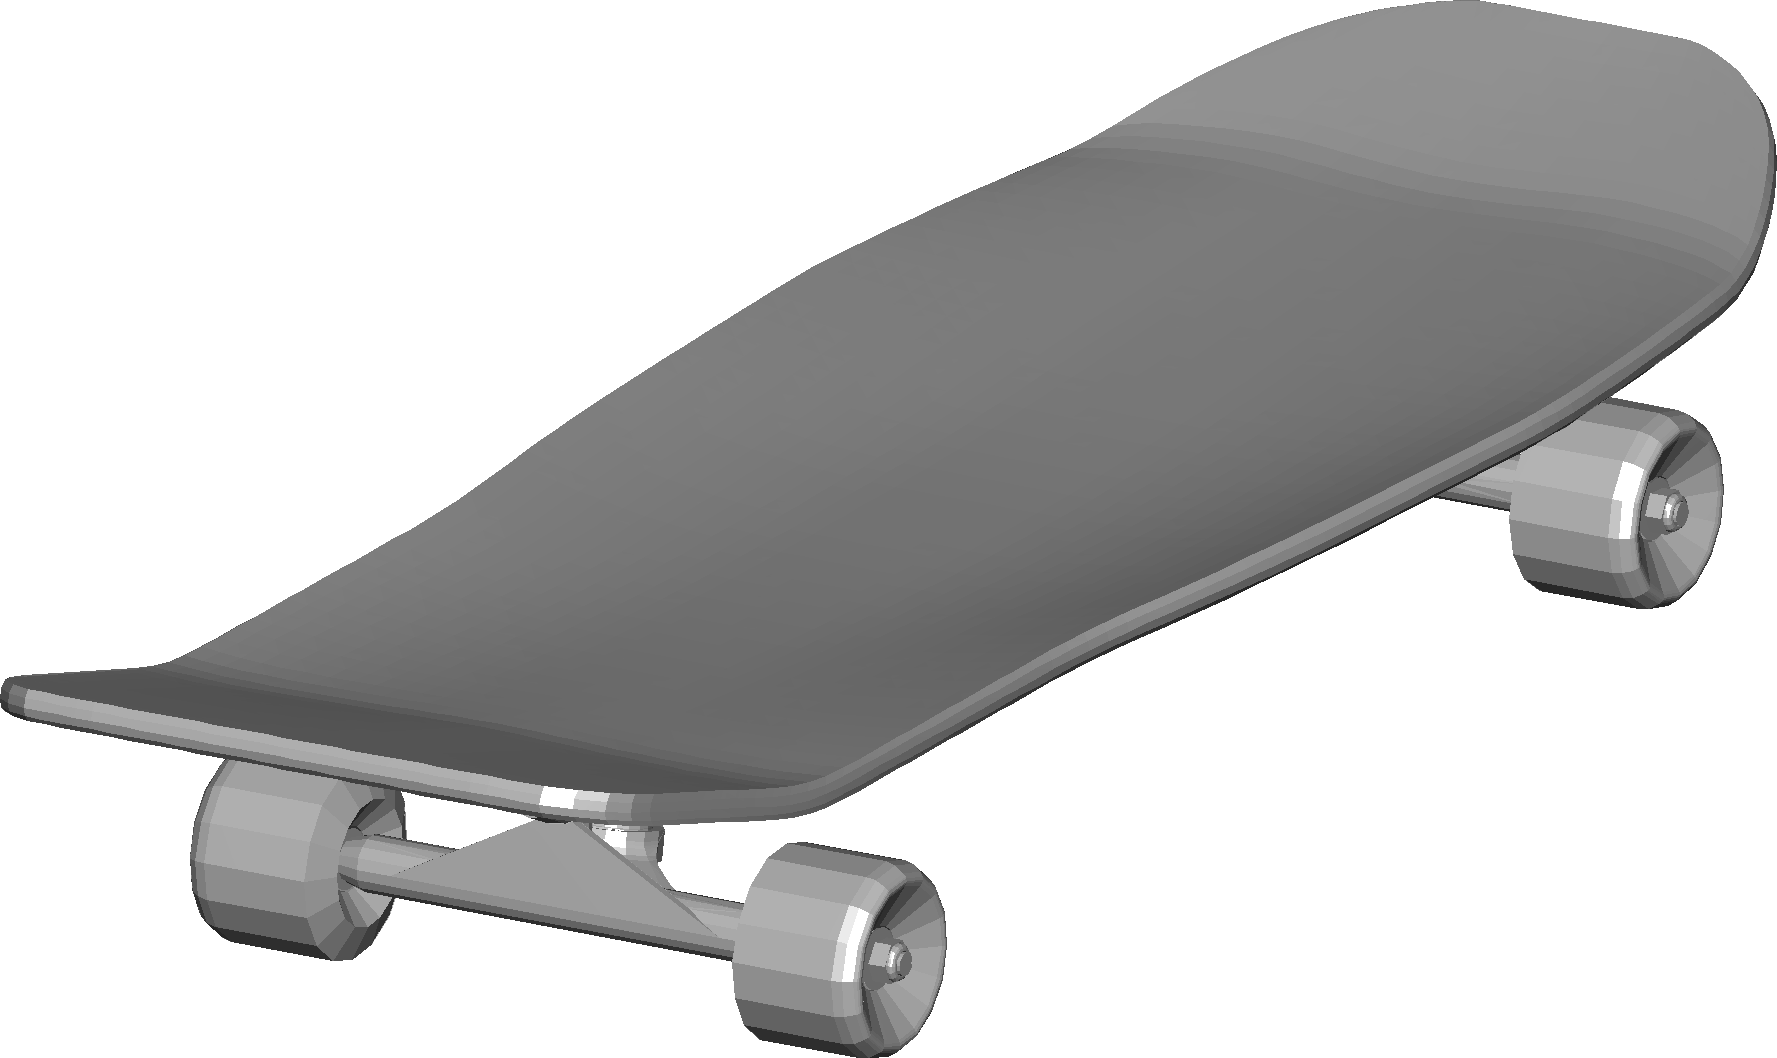
\includegraphics[width=1\linewidth]{./fig/eval/21skateboard.png}  
		\caption{Skateboard} 	
	\end{subfigure}
	\begin{subfigure}[t]{0.19\linewidth} \centering
		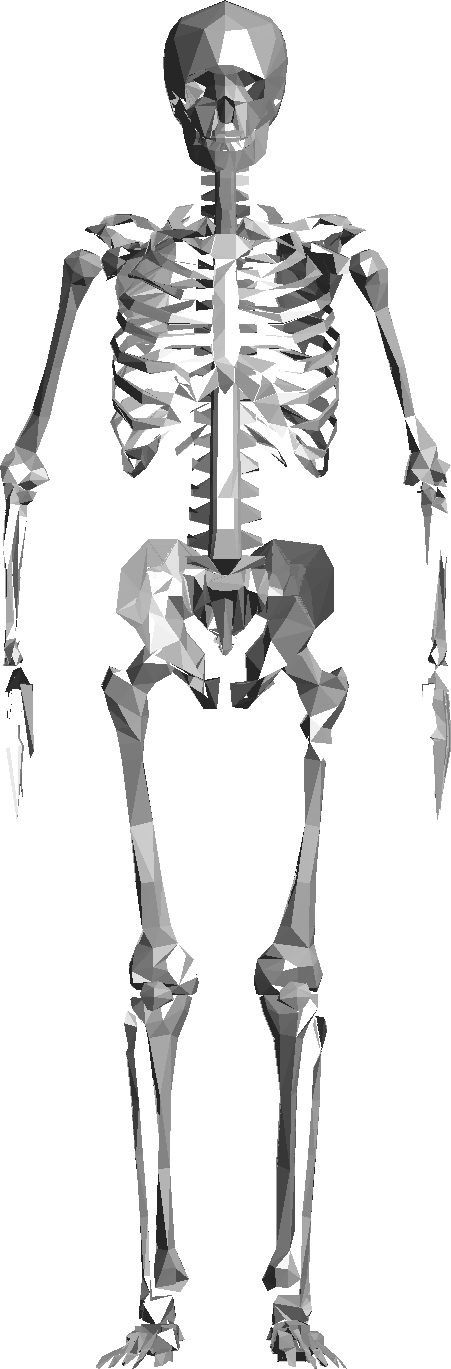
\includegraphics[width=0.3\linewidth]{./fig/eval/22skeleton.png}  
		\caption{Skeleton} 	
	\end{subfigure}
	\begin{subfigure}[t]{0.19\linewidth} \centering
		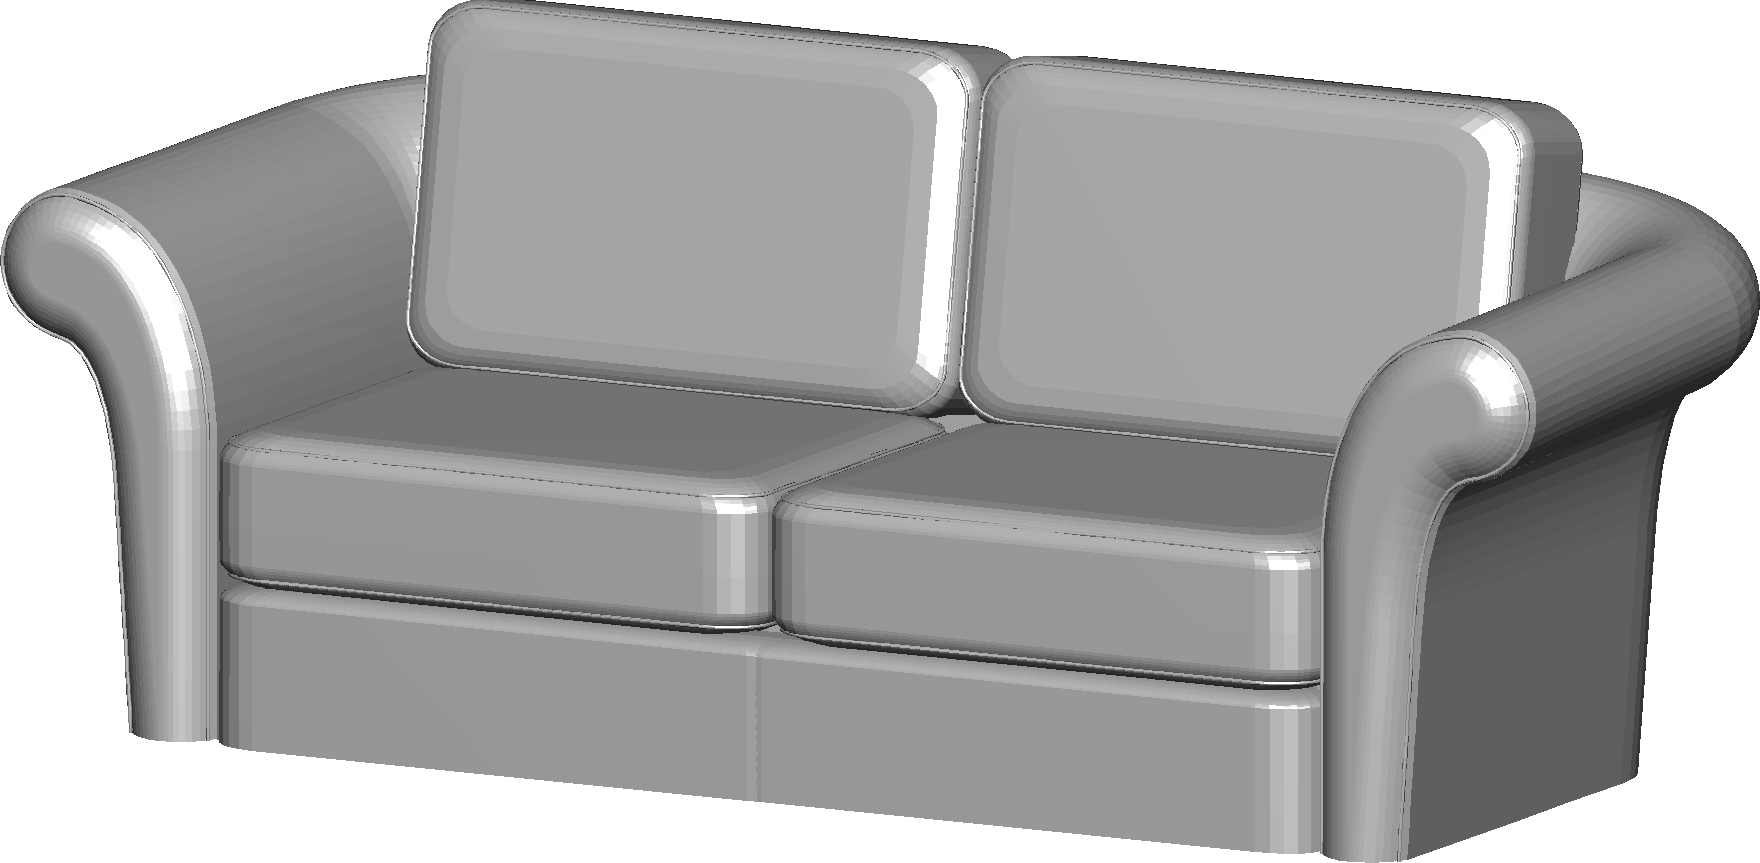
\includegraphics[width=1\linewidth]{./fig/eval/23sofa.png}  
		\caption{Sofa} 	
	\end{subfigure}
	\begin{subfigure}[t]{0.19\linewidth} \centering
		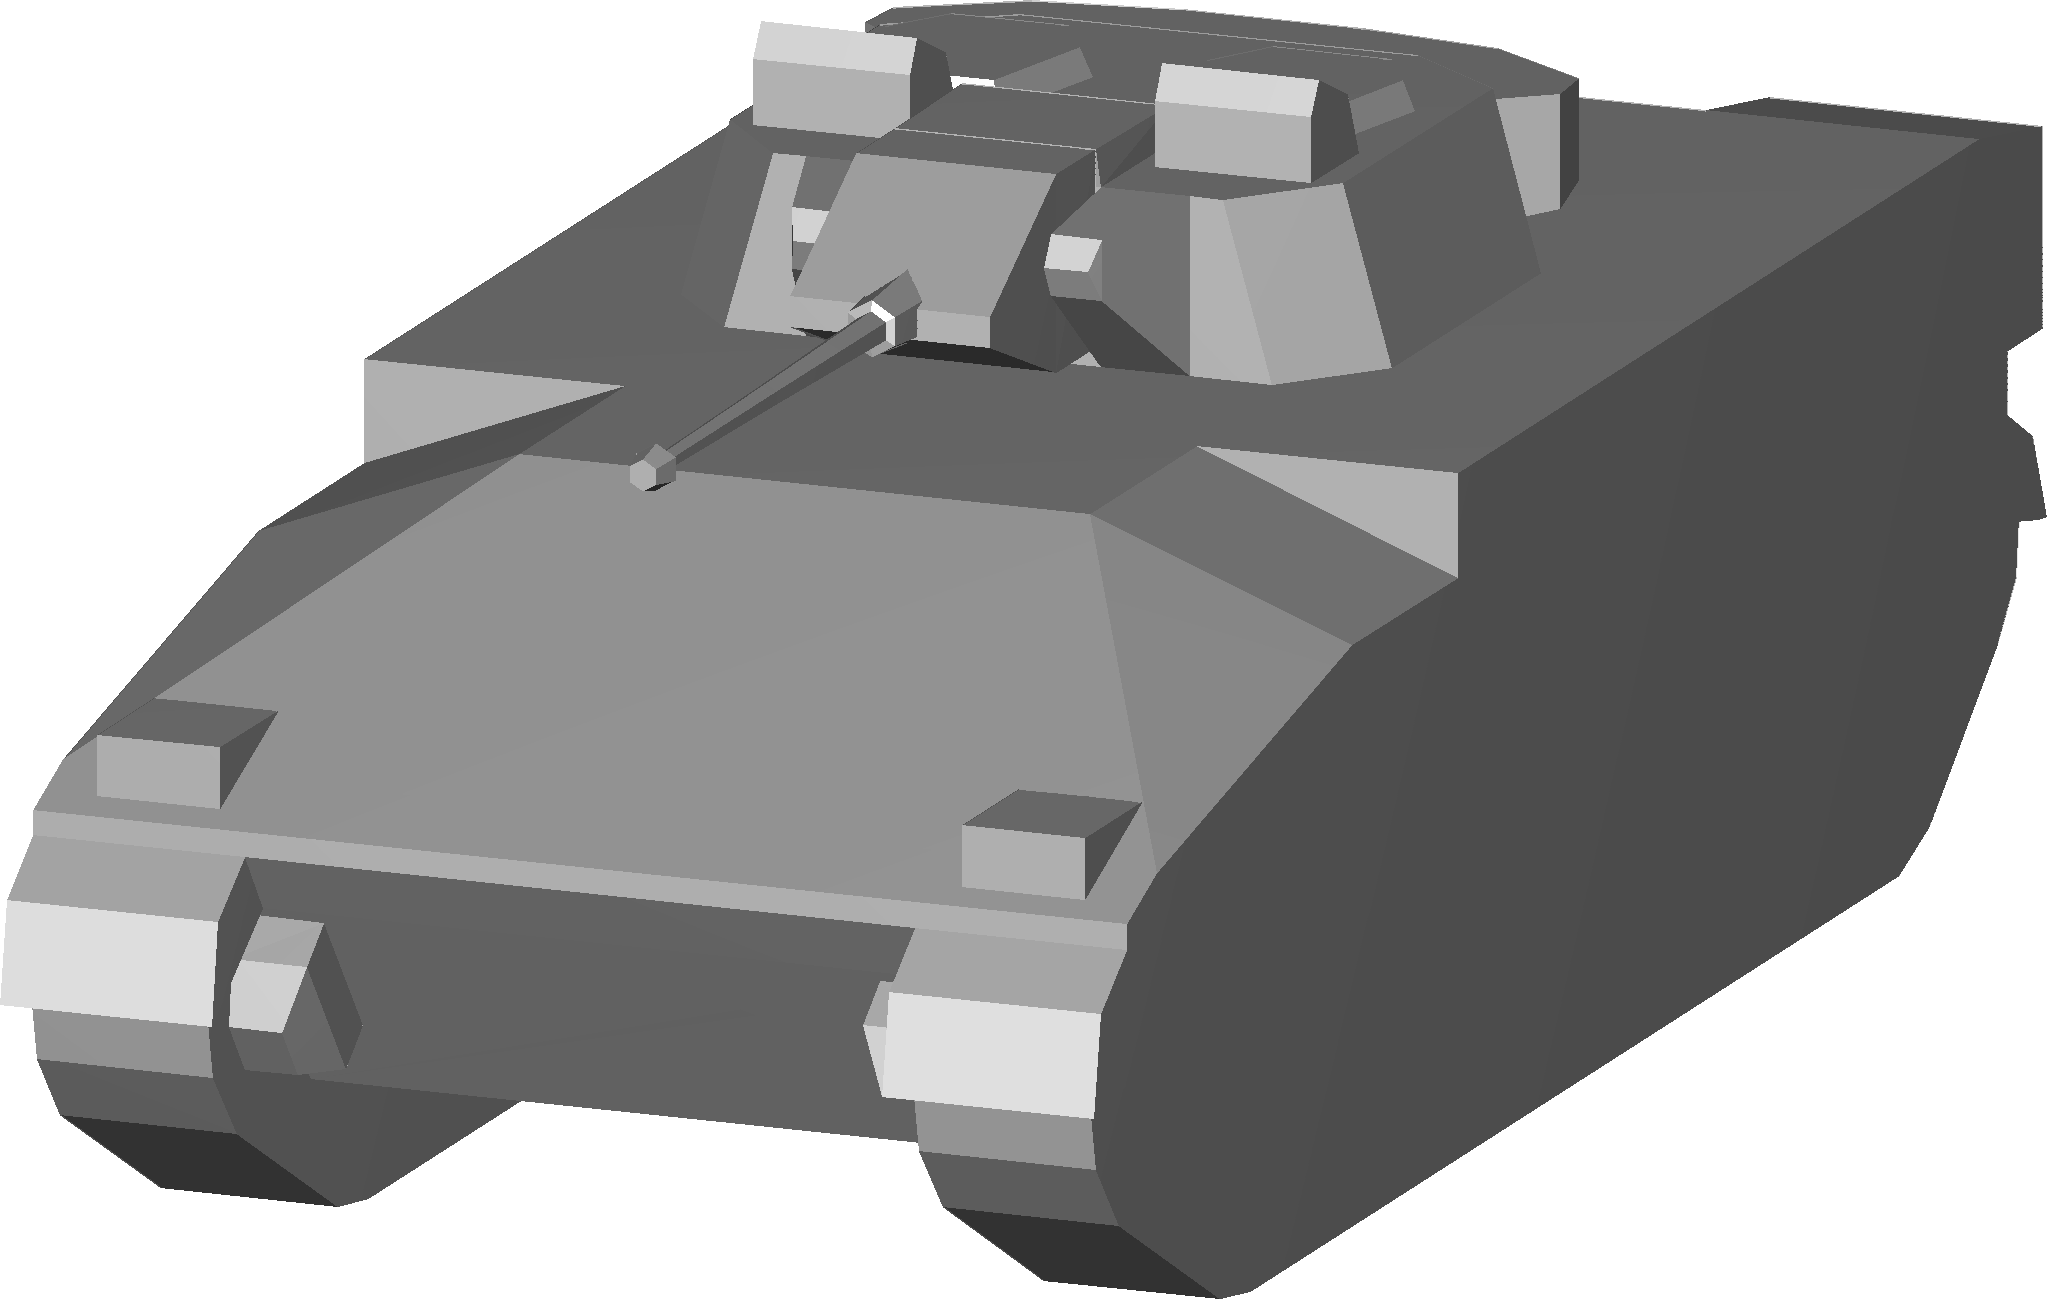
\includegraphics[width=1\linewidth]{./fig/eval/24tank.png}  
		\caption{Tank} 	
	\end{subfigure} 
	\begin{subfigure}[t]{0.19\linewidth} \centering
		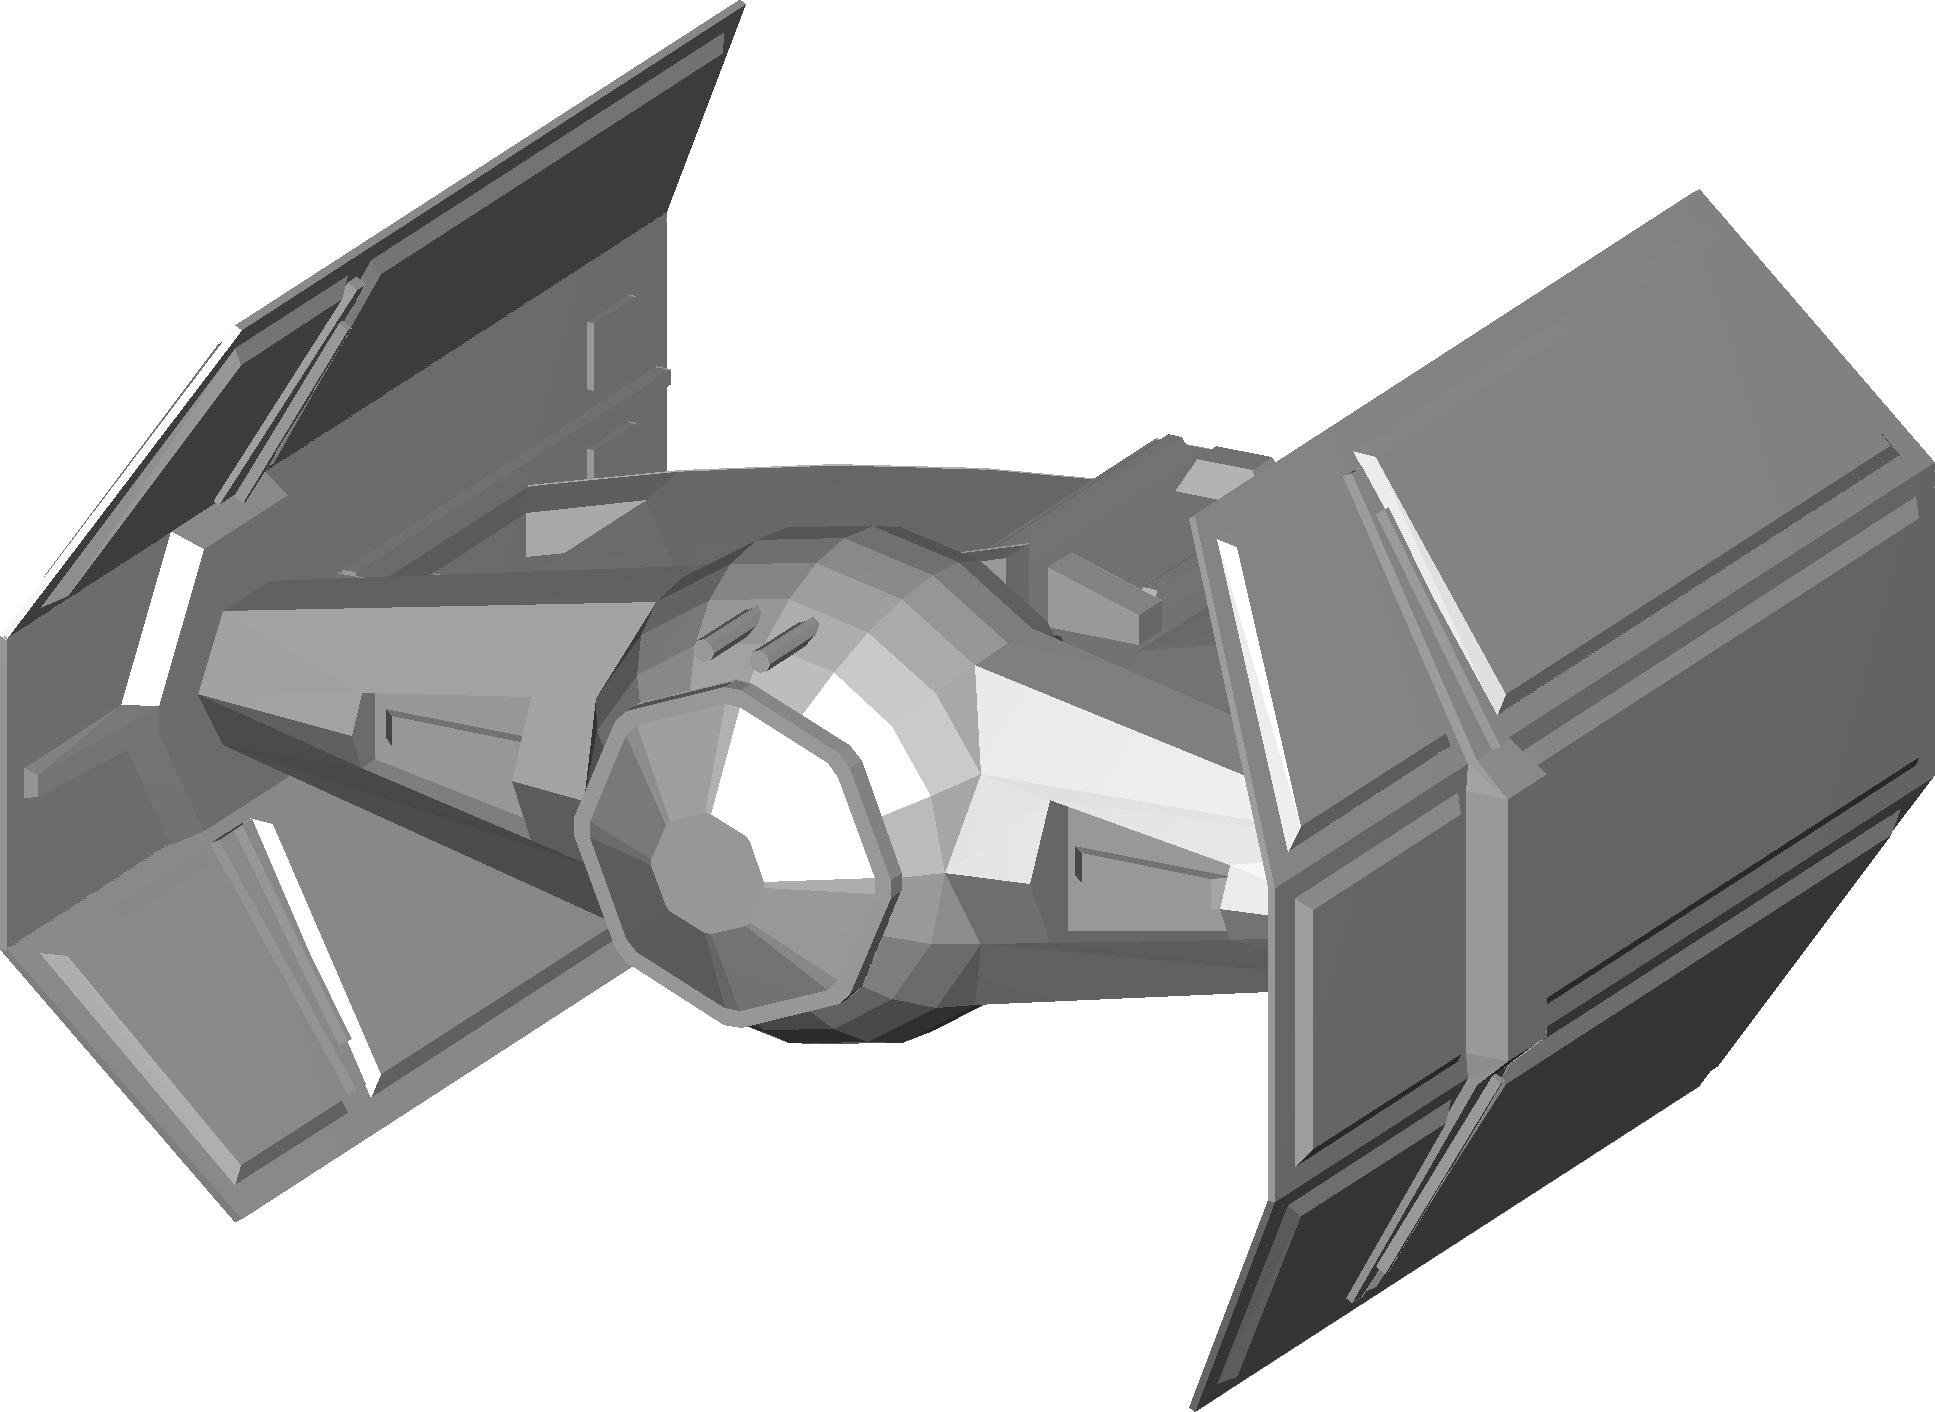
\includegraphics[width=1\linewidth]{./fig/eval/25tiefighter.png}  
		\caption{Tiefighter} 	
	\end{subfigure} 
	\caption{The sample 3D shapes in the \meshset dataset.}
	\label{fig/eval/sampleshapes}
\end{figure}


\subsection{Experimental setup}
\label{sec:variation}
In the evaluation experiments, a series of transformed shapes are created from the reference shape with different magnitudes of a test parameter. A repeatability score is computed by matching the two sets of interest points to each other, according to equation \ref{eq:rptarea}. 
The overall performance is measured by averaging the $R_{\textrm{area}}$ scores across the evaluation dataset. 

The characteristics of the interest point detectors are evaluated under several variations. 
These include rotation, translation, scale, sampling density and noise. 
Such variations are either introduced during shape acquisition (\textbf{MRI} and \textbf{Stereo} datasets), or generated synthetically (\textbf{Mesh} dataset). The variations observed in the evaluation datasets are described in table \ref{tab:datavar}. Although image compression rate and lighting change are also evaluated for image-based detectors~\cite{Mikolajczyk2005}, similar experiments are not necessary for 3D shape data because they are unaffected by such changes. 

\begin{table}
\centering
\begin{tabular}{b{1.2cm}|ccccc}
\hline
Variation/ Dataset & \textbf{Noise} & \textbf{Density} & \textbf{Scale} & \textbf{Rotation} & \textbf{Translation} \\
\hline
\textbf{Mesh} & \checkmark & \checkmark & \checkmark & \checkmark & \\
\textbf{MRI} & \checkmark & & & \checkmark & \checkmark \\
\textbf{Stereo} & \checkmark & \checkmark & \checkmark & \checkmark & \checkmark \\
\hline
\end{tabular}
\caption{Variations observed in the evaluation datasets}
\label{tab:datavar}
\end{table}

Performances of the candidate detectors are measured as each test parameter is varied individually, keeping all the other parameters at their default values. Sampling parameters (\ie noise level and sampling density) are applied to all shape instances, whilst pose parameters (\ie rotation, translation and scale) are applied to only one instance in each matching pair. Some parameters are defined in terms of $L$, the largest dimension of the voxelized reference shapes. We set the maximum value of $L$ to $200$ voxels. The default parameters for the reference shapes and the number of transformed shapes created are listed in table \ref{tab:referenceparam}. 
% For fairness of evaluation, all testing shapes share the same reference transformation. 

\begin{table}[t]
\centering
{\small
\begin{tabular}{cc}
\hline
{\textbf Parameter} & {\textbf Value} \\
\hline
\hline
\multicolumn{2}{c}{\textbf Default parameters for reference shapes } \\
Default point cloud size & $50000$ points\\
Default noise $\sigma_{n}$ & $0.0025L$\\ 
Default rotation & $0^{\circ}$\\
Maximum $L$ & $200$ voxels\\
Default $\sigma_{\textrm{KDE}}$ in $g(\cdot,\sigma_{\textrm{KDE}})$ & $1.5$ voxels \\ 
Distance threshold $D$ & $0.03L$ \\
Parameter $f$ in equation (\ref{eq:loc_vec}) & $\sqrt{8}$ \\
Number of octaves in scale-space & $4$ \\
\hline
\multicolumn{2}{c}{ {\textbf Number of transformed shapes compared }} \\
Sampling noise & 13 \\
Sampling density & 17 \\
Noise & 21 \\
Scale & 21 \\
\hline
\end{tabular}
}
\caption{The reference parameters for the testing shapes.}
\label{tab:referenceparam}
\end{table}

\subsection{Experiments on synthetic meshes}

\begin{figure}[ht]
\centering
\subfloat[$\sigma_{n} = 0$]{
	\label{fig:noise_none}
	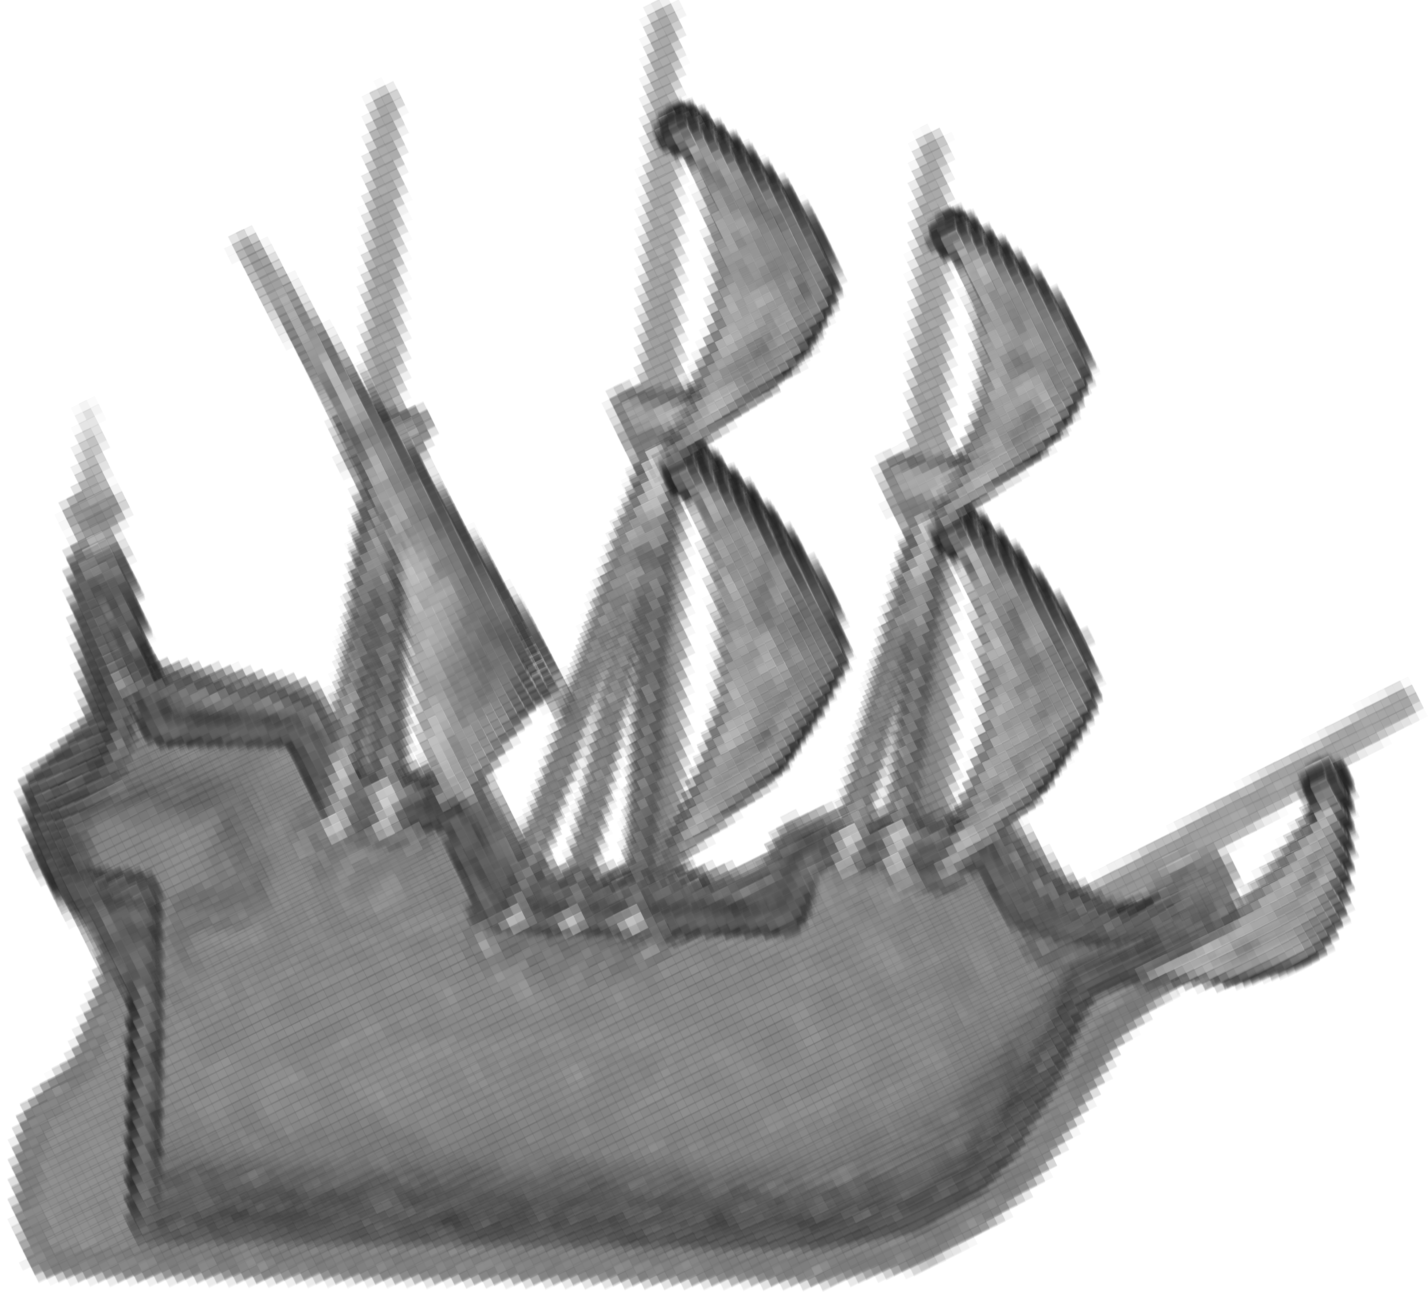
\includegraphics[width=0.22\linewidth]{./fig/eval/noise_none.png}
}
\subfloat[$\sigma_{n} = 0.0025L$]{
	\label{fig:noise_low}
	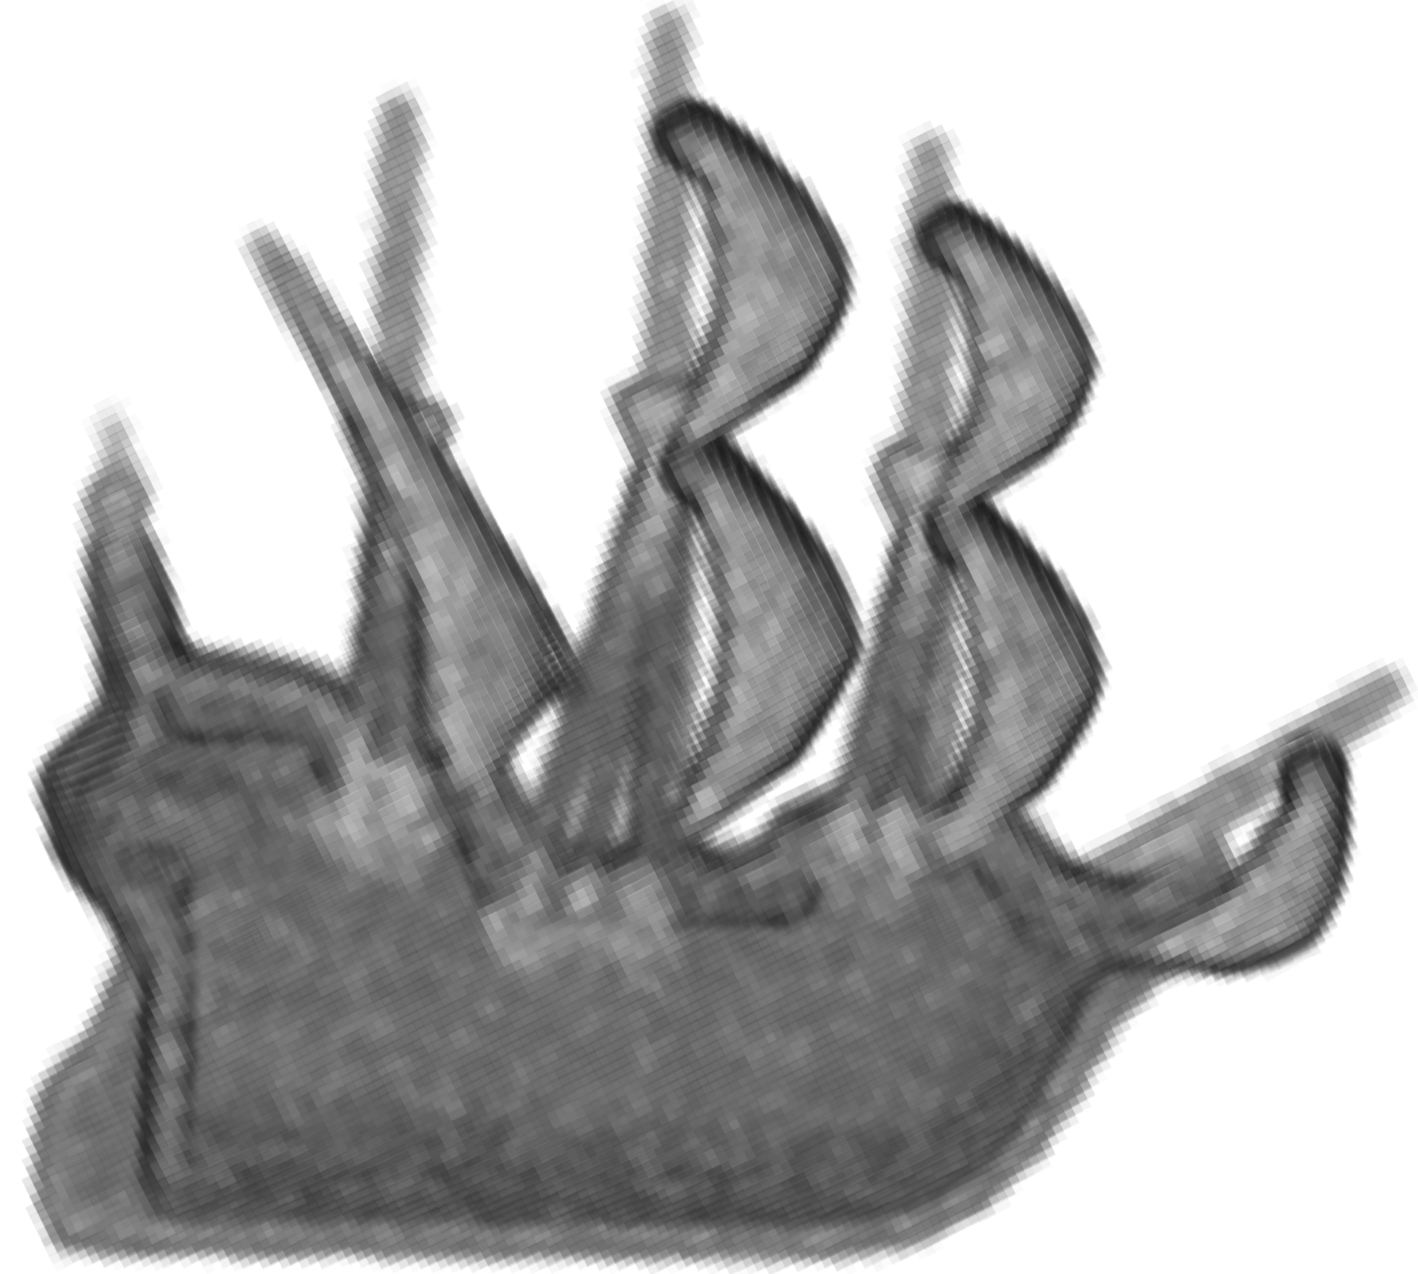
\includegraphics[width=0.22\linewidth]{./fig/eval/noise_low.png}
}
\subfloat[$\sigma_{n} = 0.01L$]{
	\label{fig:noise_mid}
	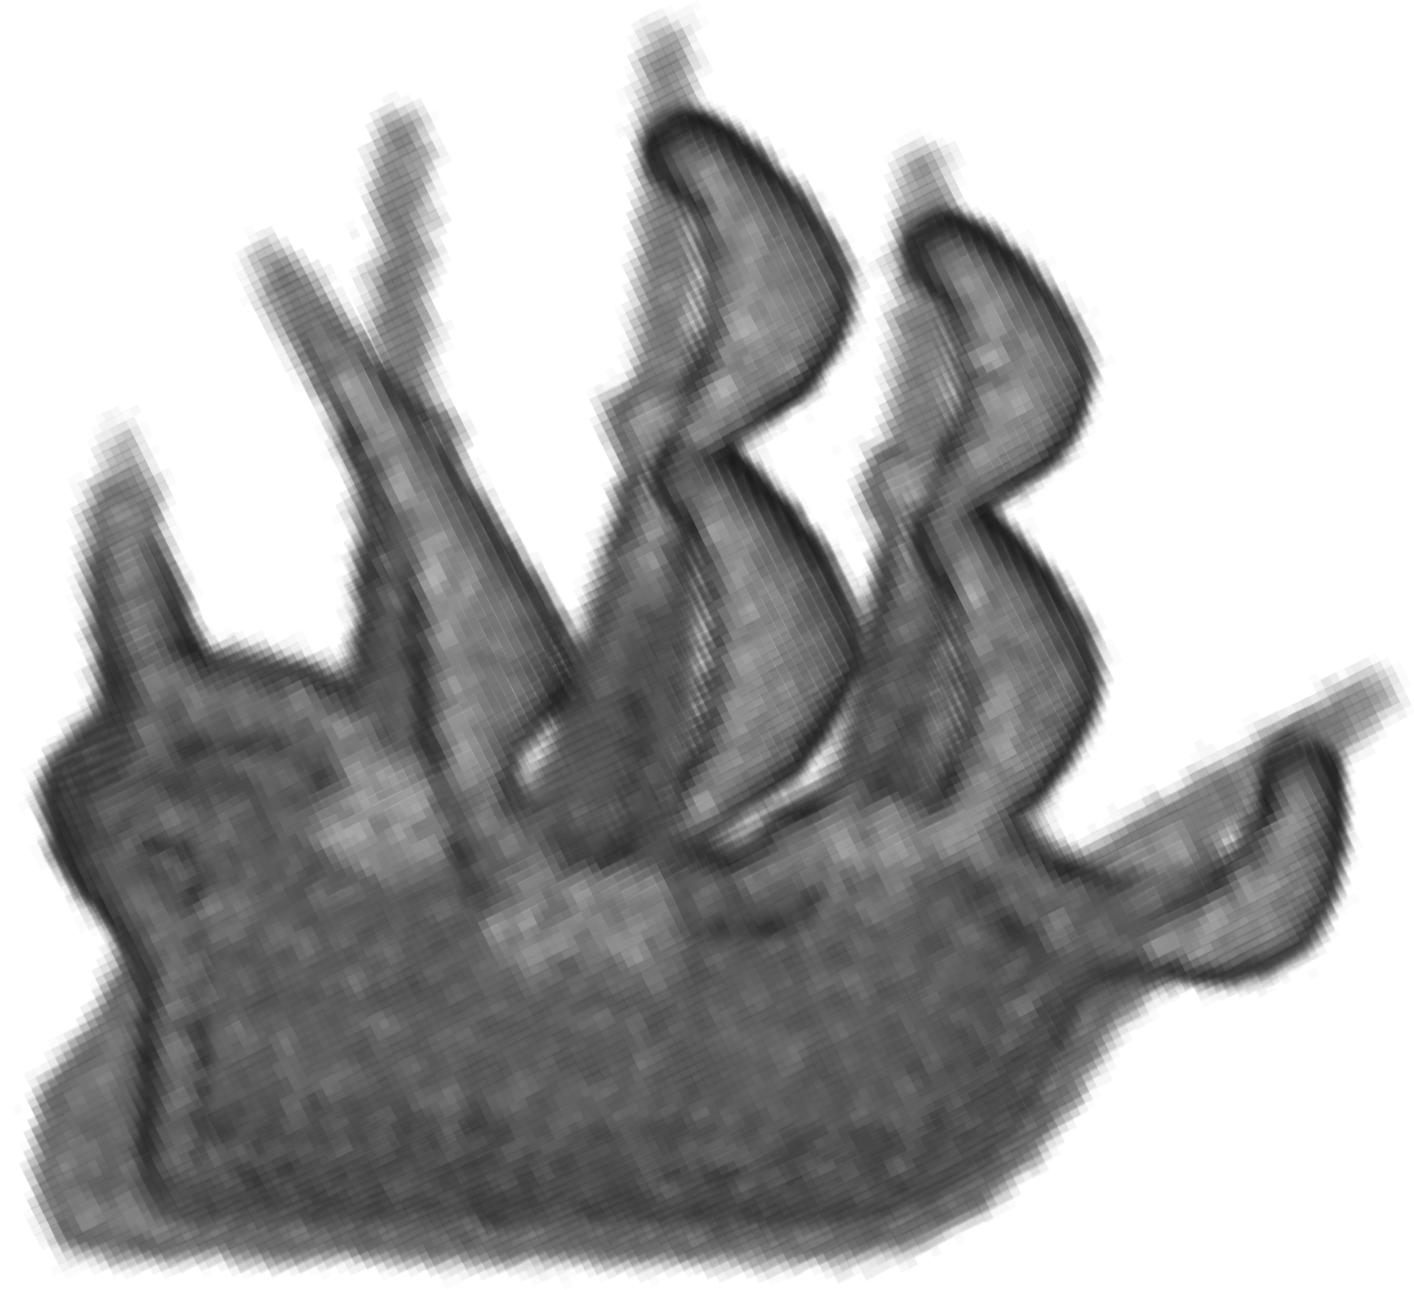
\includegraphics[width=0.22\linewidth]{./fig/eval/noise_mid.png}
}
\subfloat[$\sigma_{n} = 0.02L$]{
	\label{fig:noise_high}
	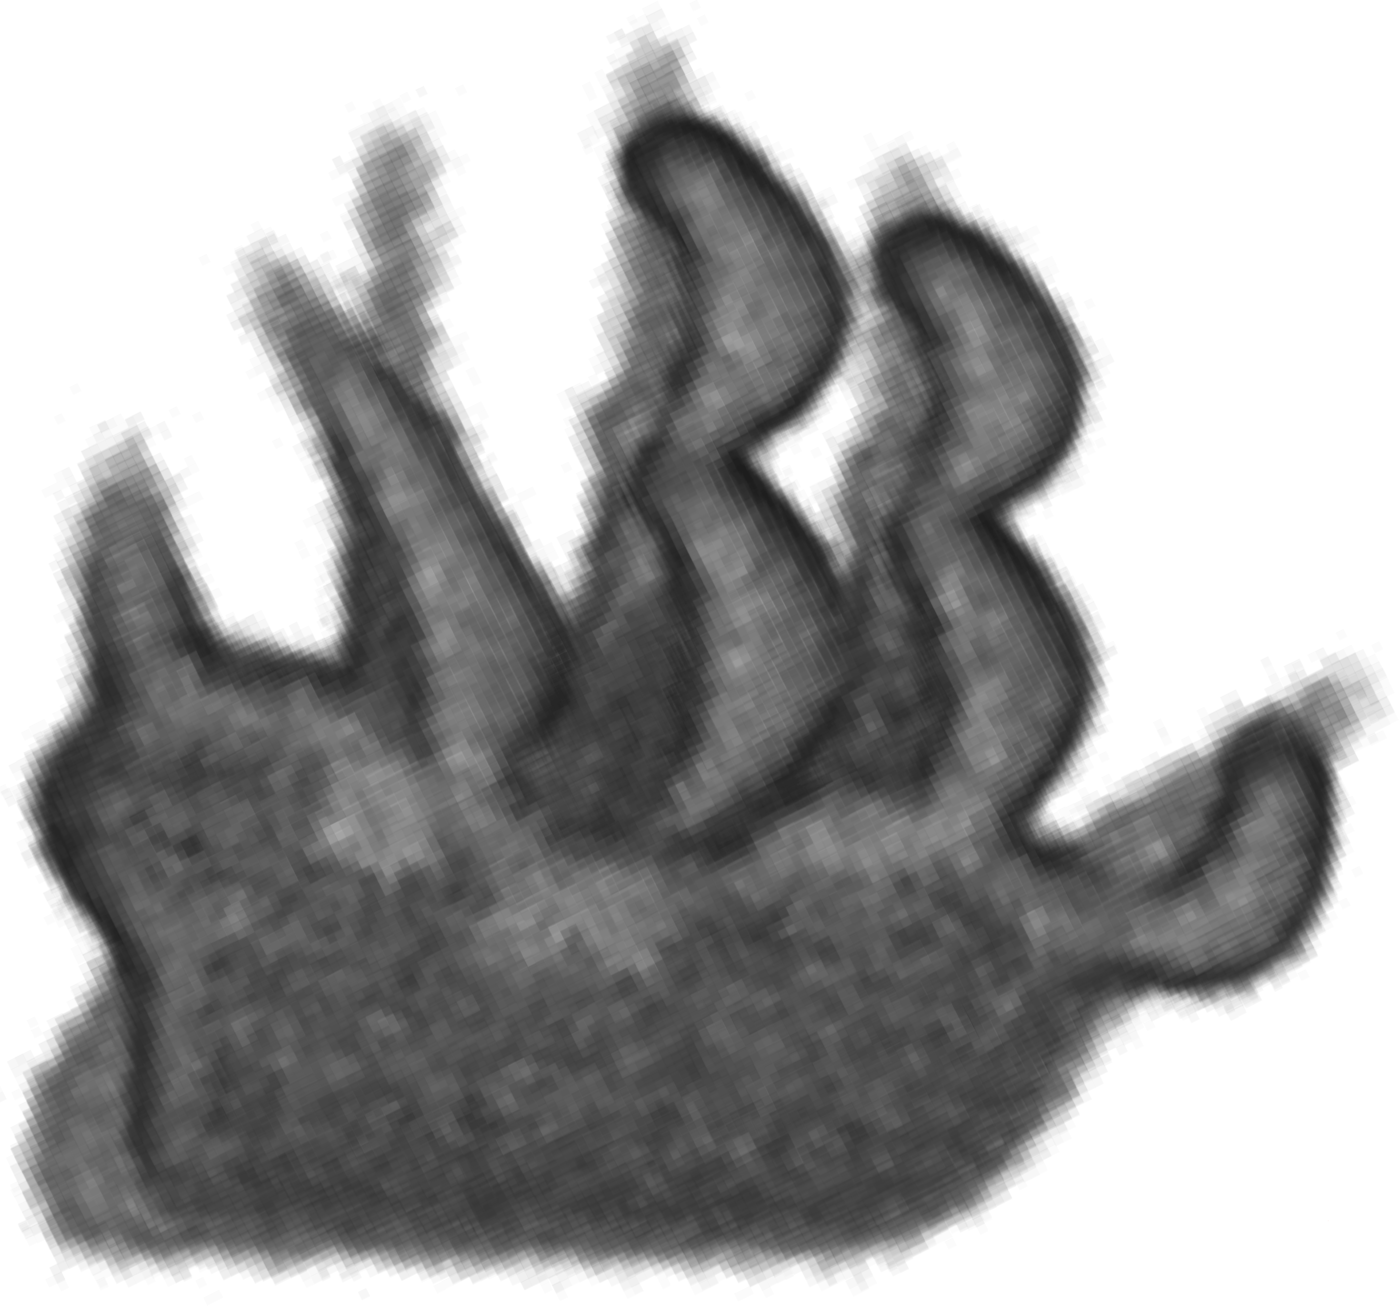
\includegraphics[width=0.22\linewidth]{./fig/eval/noise_high.png}
}
\vspace{-4mm}
\caption{The ``galleon'' shape from the \textbf{Mesh} dataset, with different levels of sampling noise. Note that the shape details disappear gradually as the noise level increases.}
\label{fig:noisesample}
\end{figure}

\subsubsection{Sampling noise}

Sampling noise and density are crucial factors in 3D interest point detection. As most of the 3D data acquisition techniques rely on shape reconstruction from point clouds or tomograms, existing shape acquisition techniques (\eg multi-view stereo, 3D ultrasound) often produce data with sampling noise. 
In this test, different levels of Gaussian white noise, with standard deviations $\sigma_{n}$ from $0L$ to $0.03L$, are applied to the {\textbf Mesh} dataset.

The result is shown in figure \ref{fig:graph_noise}. MSER outperforms other interest points, demonstrating high robustness. While the $R_{\textrm{area}}$ scores of other detectors decline rapidly,
MSER still achieves a high $R_{\textrm{area}}$ score. The DoH detector shows a relatively stronger tolerance than detectors like SURF, Harris and V-FAST. In contrast, the SURF detector has almost zero points matched when sampling noise is more than $6.5\%L$.

\subsubsection{Sampling density}

The $R_{\textrm{area}}$ score of shapes with various sampling densities are measured. Point clouds are randomly sampled from the input meshes, with point cloud sizes ranging from $4$K points to $405$K points. The sampling density of a point cloud directly affects its voxelization process, loss of details and holes are usually observed in point clouds in low sampling densities. 

Figure \ref{fig:graph_sample} presents the change of $R_{\textrm{area}}$ scores versus point cloud size. The scores vary linearly in log scale, therefore a diminishing return is observed with increasing sampling density. MSER achieves the best average performance but it also has the largest variance across different shapes. DoH and DoG produce satisfactory results, with high scores but smaller intra-dataset variance than that of MSER.

\subsubsection{Rotation}

This experiment evaluates susceptibility of the detectors to rotational aliasing effects. 
For each magnitude of rotation angle, an average $R_{\textrm{area}}$ score is computed by matching the testing shapes multiple times using different rotation axes, making the evaluation results unbiased. Eight rotation axes are generated randomly for each shape, and rotations of increasing magnitude, up to $90^\circ$, applied about them. 

The effect of rotation is shown in figure \ref{fig:graph_rotation}. Most detectors show excellent tolerance to rotation, inheriting this from their image-based counterparts. 
DoG and MSER perform slightly better than others, with very stable average score over a broad range of rotation angles. SURF performs worse than other volumetric interest point because the use of box filters introduces quantization errors when the shapes are rotated.

\subsubsection{Scale}

Dimensions of voxelized input data are scaled from $50\%$ to $200\%$ of their original sizes. For fairness of evaluation, the transformed shapes are not directly interpolated from their voxelized reference shapes. Rather, input point clouds are re-voxelized with varying volume dimensions $L$, whilst other parameters remain unchanged. 

The values of $R_{\textrm{area}}$ measured against scale changes are illustrated in figure \ref{fig:graph_scaling}. DoG and DoH detectors are comparatively more robust to scale. SURF only works well at $100\%$ and drops outside the original scale, because of the approximated scale-space used. MSER achieves the best result at its original size, yet its performance decreases steadily when the shape is scaled.
Repeatability scores of all detectors drop faster in downsampled volumes (scale $< 100\%$) than in upsampled volumes (scale $> 100\%$). 
This is due to the information of smaller shape features being lost when the input volume is downsampled. In addition, the scale-space does not cover any feature with size smaller than the first octave, therefore fine details are undetected.  
Similarly, the performance of most detectors drops slowly at scale $> 100\%$, when some features become too large to be detected. 

\begin{table}[t]
\centering
\begin{tabular}{c|ccc}
\hline
Avg.\# Pts. & \multicolumn{3}{c}{\textbf Sampling Noise Level}  \\
Avg.\# Corr.Pts. &  {\textbf Low}  & {\textbf Medium}  & {\textbf High}  \\
({\textit Corr. \%}) & ($0.0025L$) & ($0.01L$) & ($0.02L$) \\
\hline
\hline
\multirow{3}{*}{\textbf DoG}  &   122.0 & 118.2 & 73.1 \\
&  48.8 & 35.1 &  9.3 \\
& ({\textit{\textit 39.8\%}}) & ({\textit 29.7\%}) & ({\textit 12.7\%}) \\
\hline
\multirow{3}{*}{\textbf SURF} &  154.7 & 70.4  & 28.7 \\
&  54.7 & 18.4  & 3.84 \\
&  ({\textit35.3\%}) & ({\textit26.2\%})  & ({\textit 13.4\%}) \\
\hline
\multirow{3}{*}{\textbf Harris} & 303.3 & 142.2 &  123.8 \\
& 78.6  & 33.2  &    13.4  \\
& ({\textit 25.9\%}) & ({\textit 23.3\%}) & ({\textit 10.83\%}) \\
\hline
\multirow{3}{*}{\textbf DoH}&  {\textbf\underline{330.8}} & {\textbf\underline{272.0}} &   {\textbf\underline{201.2}} \\
&  {\textbf\underline{117.1}} & {\textbf\underline{72.2}}  &   {\textbf\underline{30.2}} \\
& ({\textit35.4\%}) & ({\textit26.6\%}) & ({\textit 18.2\%}) \\
\hline
\multirow{3}{*}{\textbf V-FAST}&  115.9 &  85.5  &  74.6\\ 
&  33.5  & 15.5  &    7.4 \\
& ({\textit 28.8\%}) & ({\textit 18.10\%})  & ({\textit 9.85\%}) \\
\hline
\multirow{3}{*}{\textbf MSER} &  99.0  & 74.4  &   52.5 \\
&  59.9 & 44.7  &   28.8 \\
& ({\textit{\textbf\underline{60.5}}\%})  & ({\textit{\textbf\underline{60.2}}\%})  & ({\textit{\textbf\underline{54.9}}\%})\\
\hline
\end{tabular}
\caption{\emph{For each entry, top to bottom:} The average number of interest points detected, the average number of correspondences ($d \le 0.015L$), percentage of points with correspondences.}
\label{tab:numcorr}
\end{table}

\subsubsection{Number of corresponding interest points}

\begin{figure}[ht]
\centering
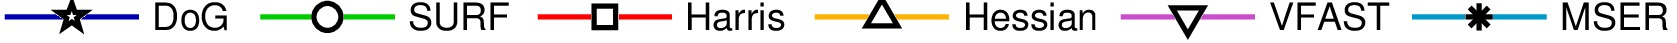
\includegraphics[width=0.70\linewidth]{./fig/eval/hlegend.jpg}\\
\subfloat[Sampling Noise]{
	\label{fig:graph_noise}
	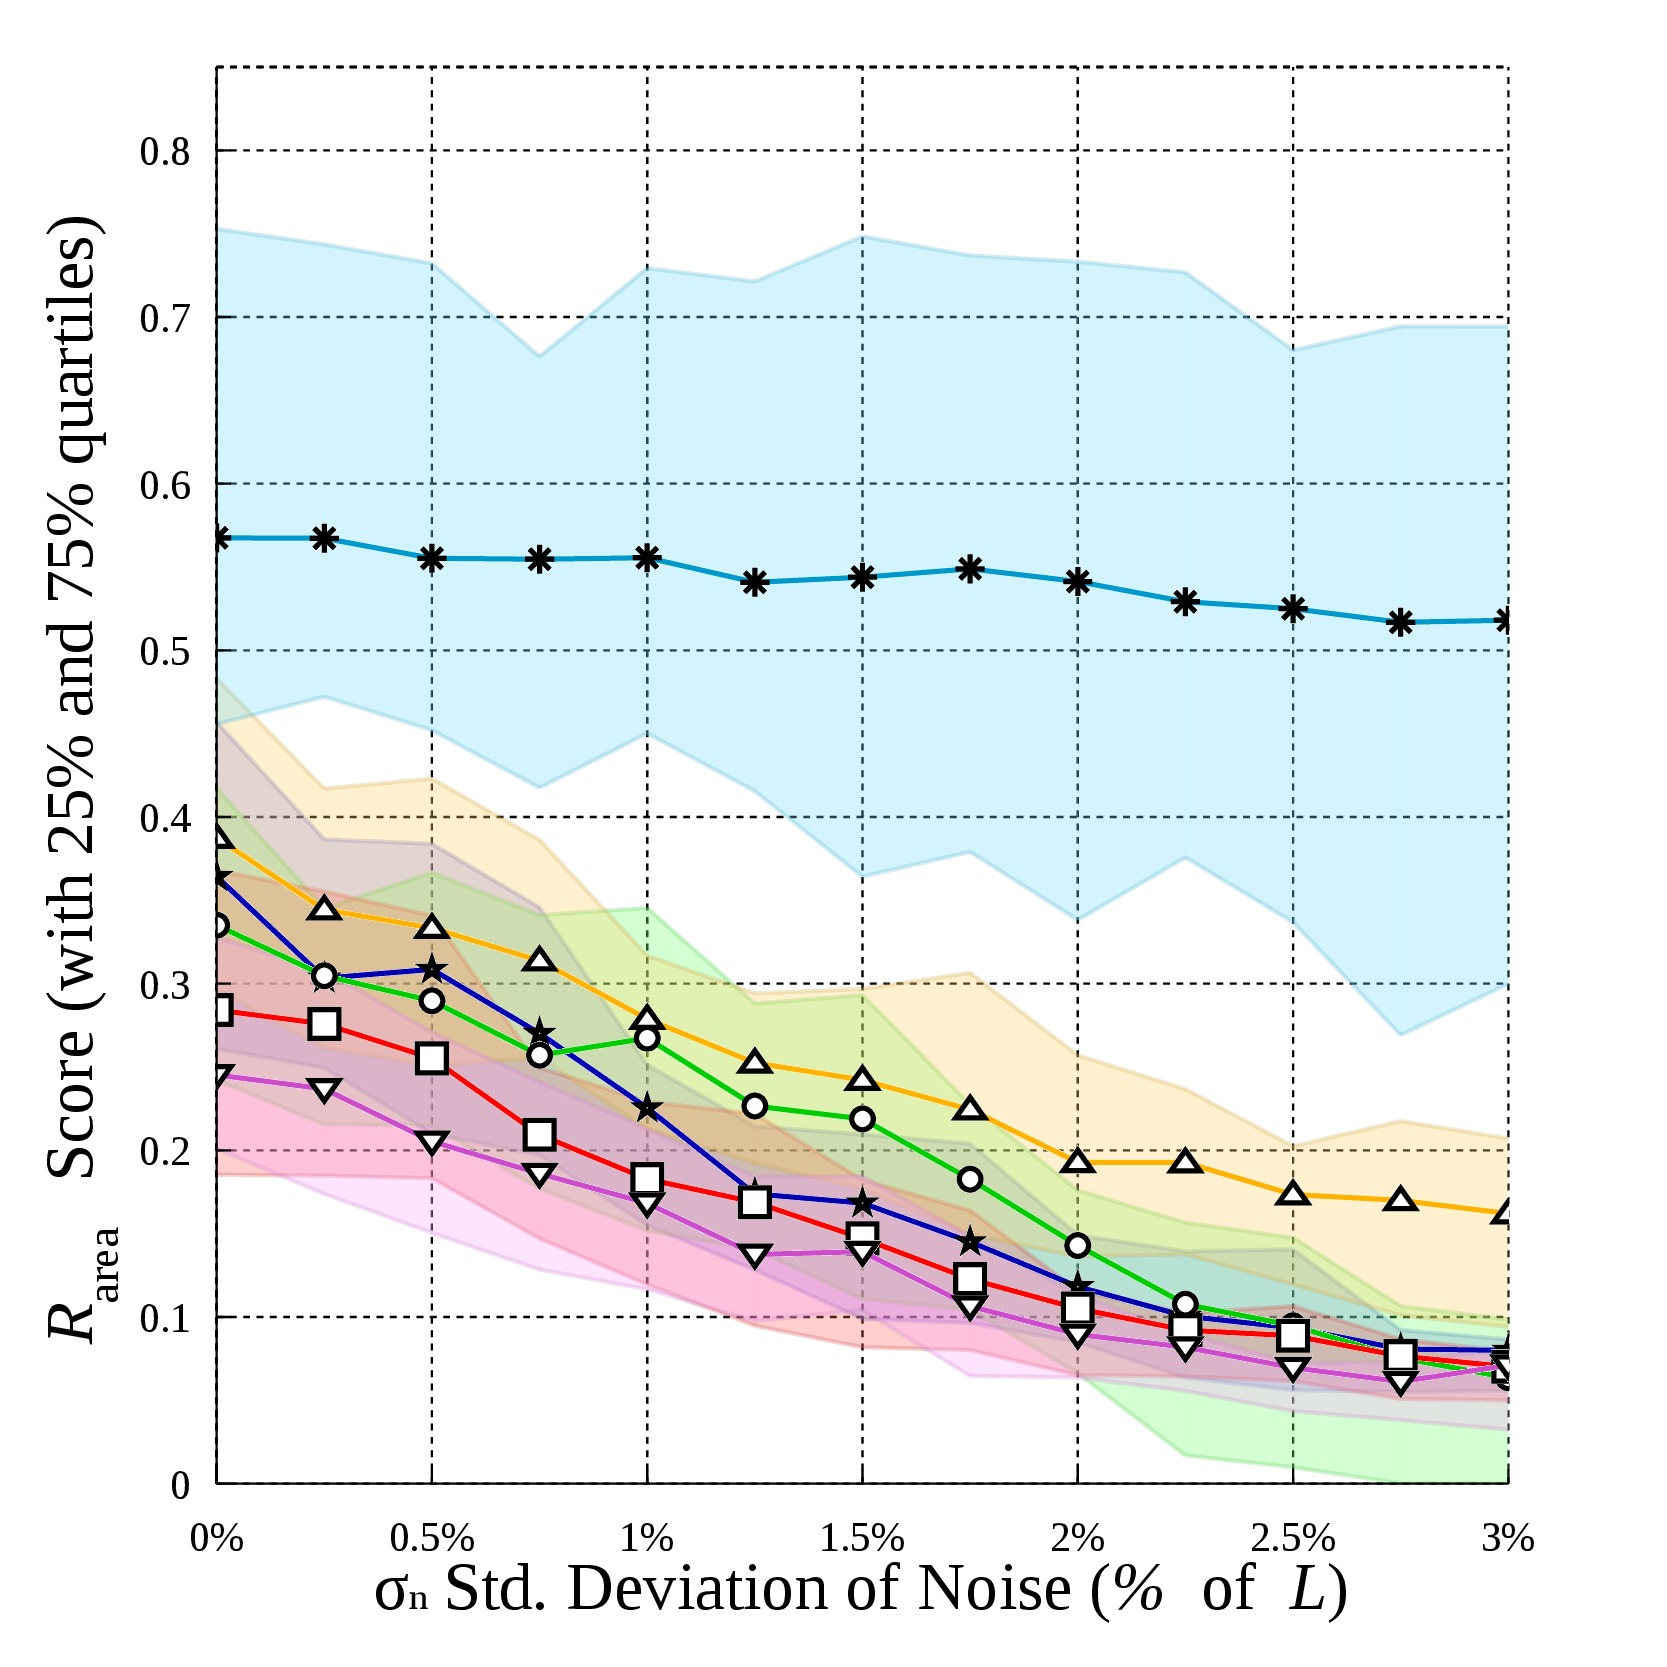
\includegraphics[width=0.33\linewidth]{./fig/eval/graph_noise.jpg}
}
\subfloat[Sampling Density]{
	\label{fig:graph_sample}
	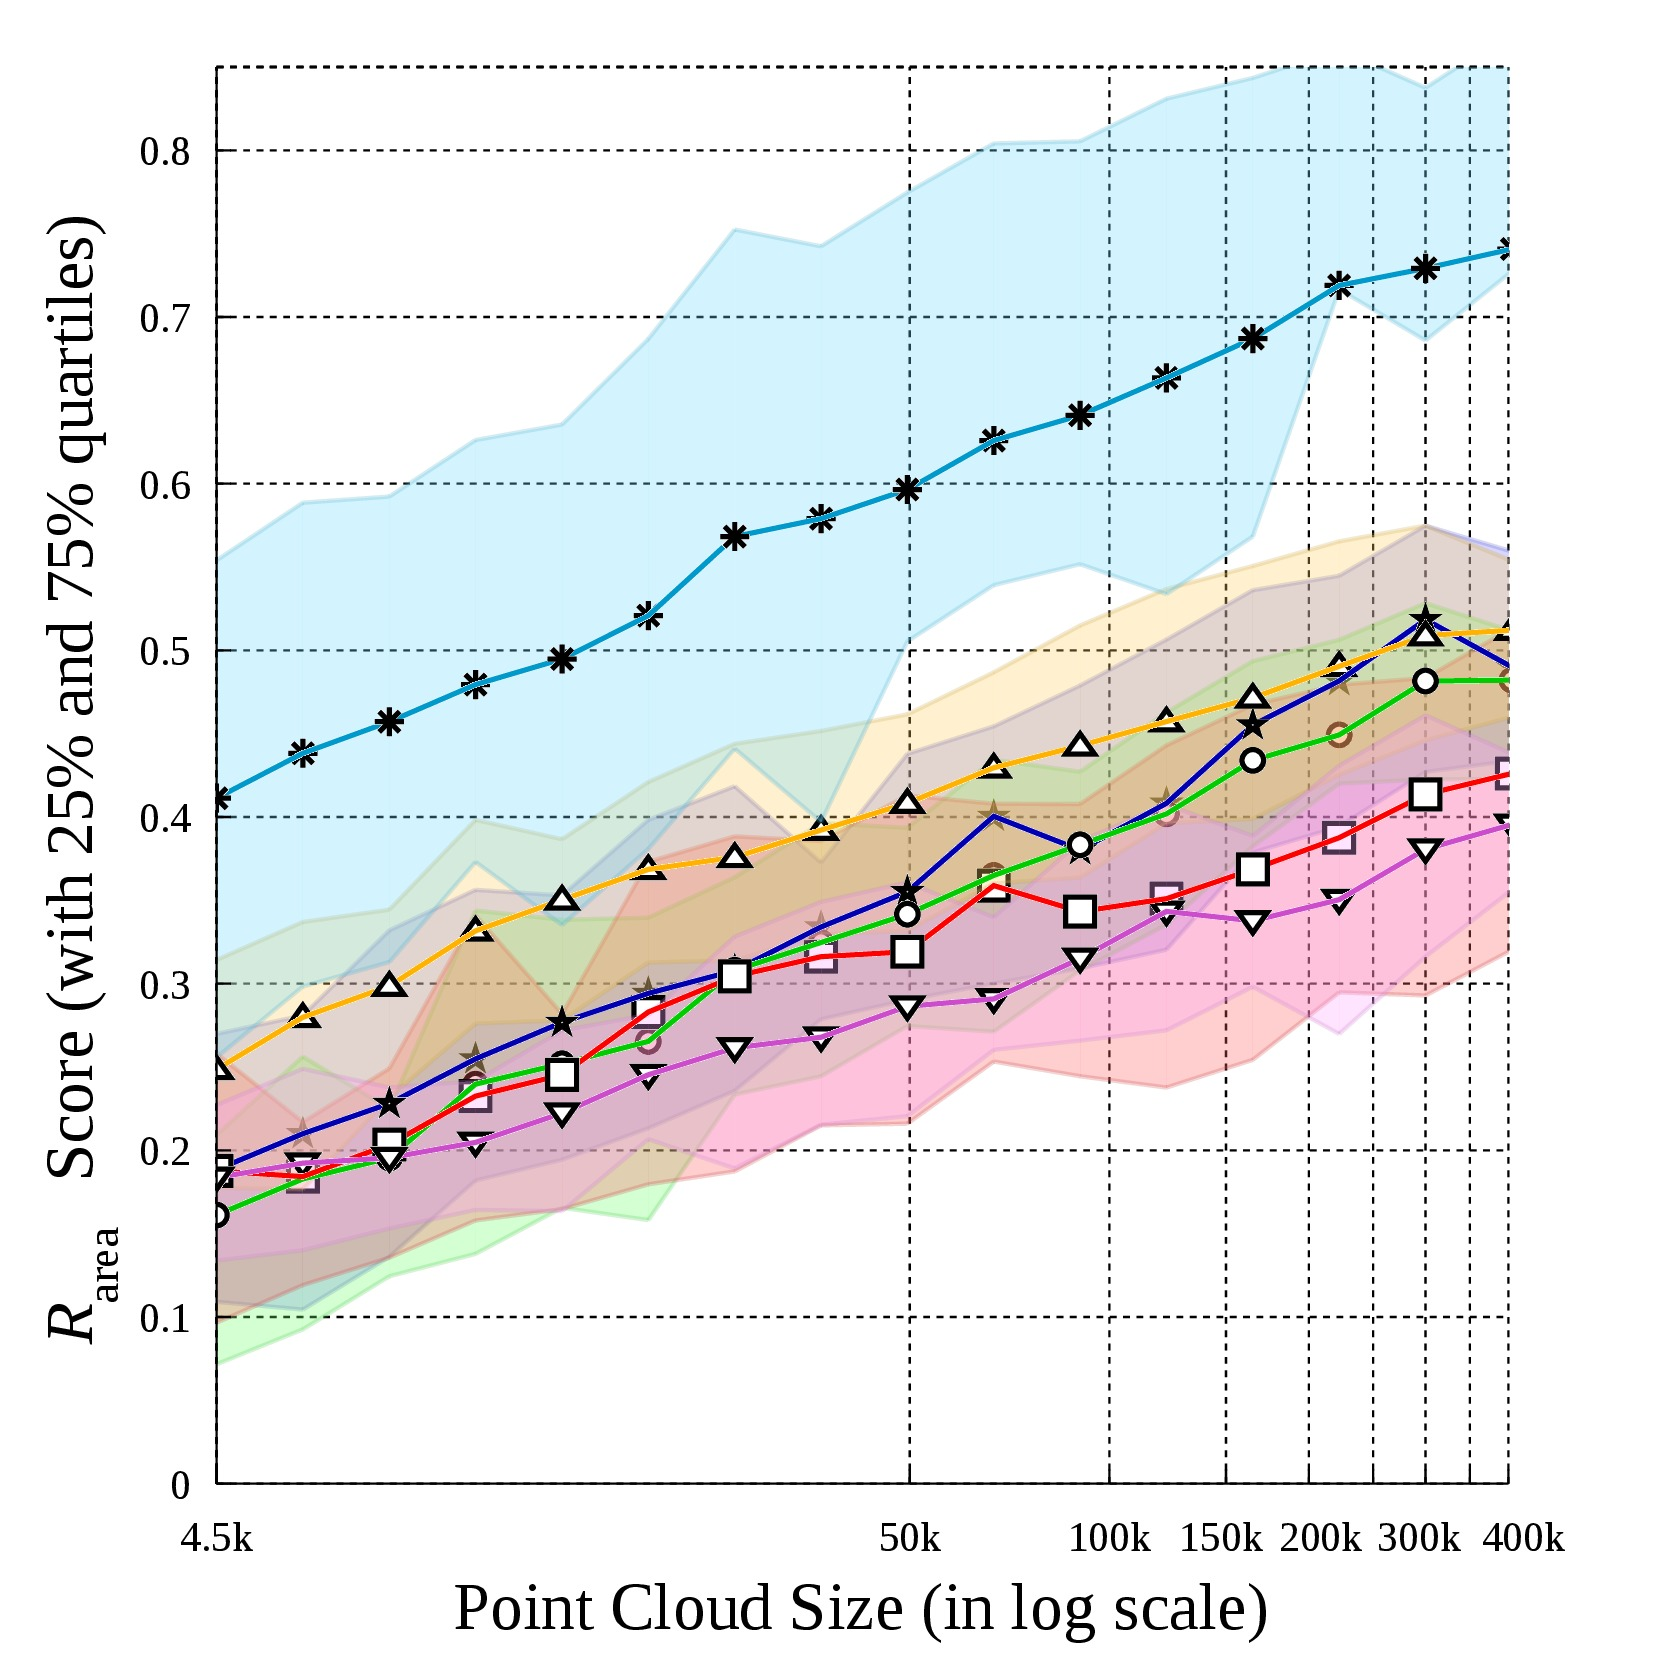
\includegraphics[width=0.33\linewidth]{./fig/eval/graph_sampling.jpg}
}
\subfloat[Rotation]{
	\label{fig:graph_rotation}
	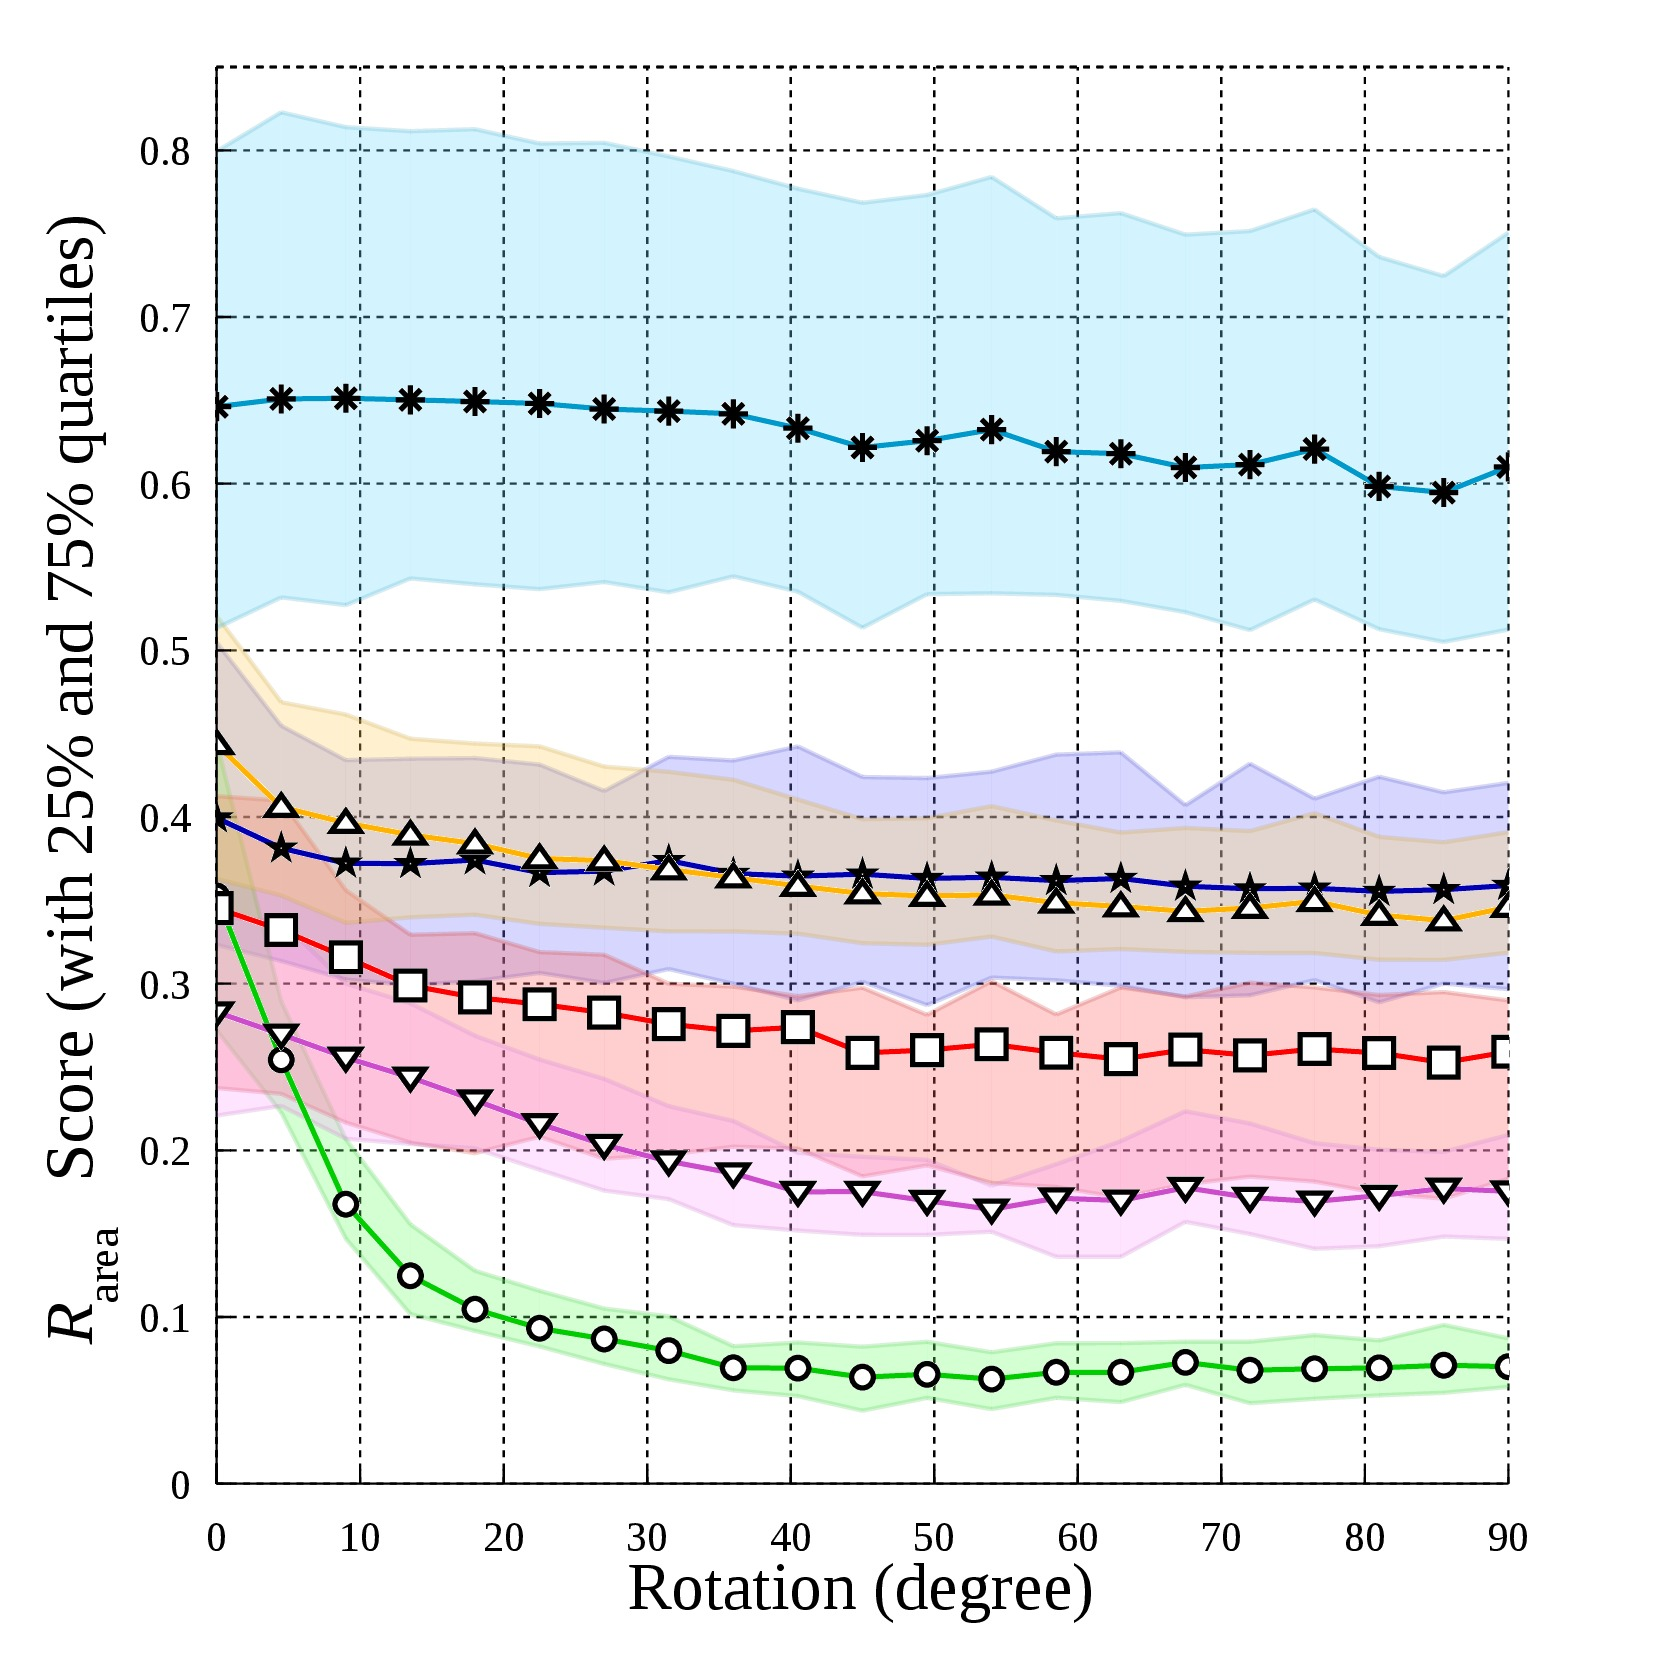
\includegraphics[width=0.33\linewidth]{./fig/eval/graph_rotation.jpg}
} \\
\subfloat[Scale]{
	\label{fig:graph_scaling}
	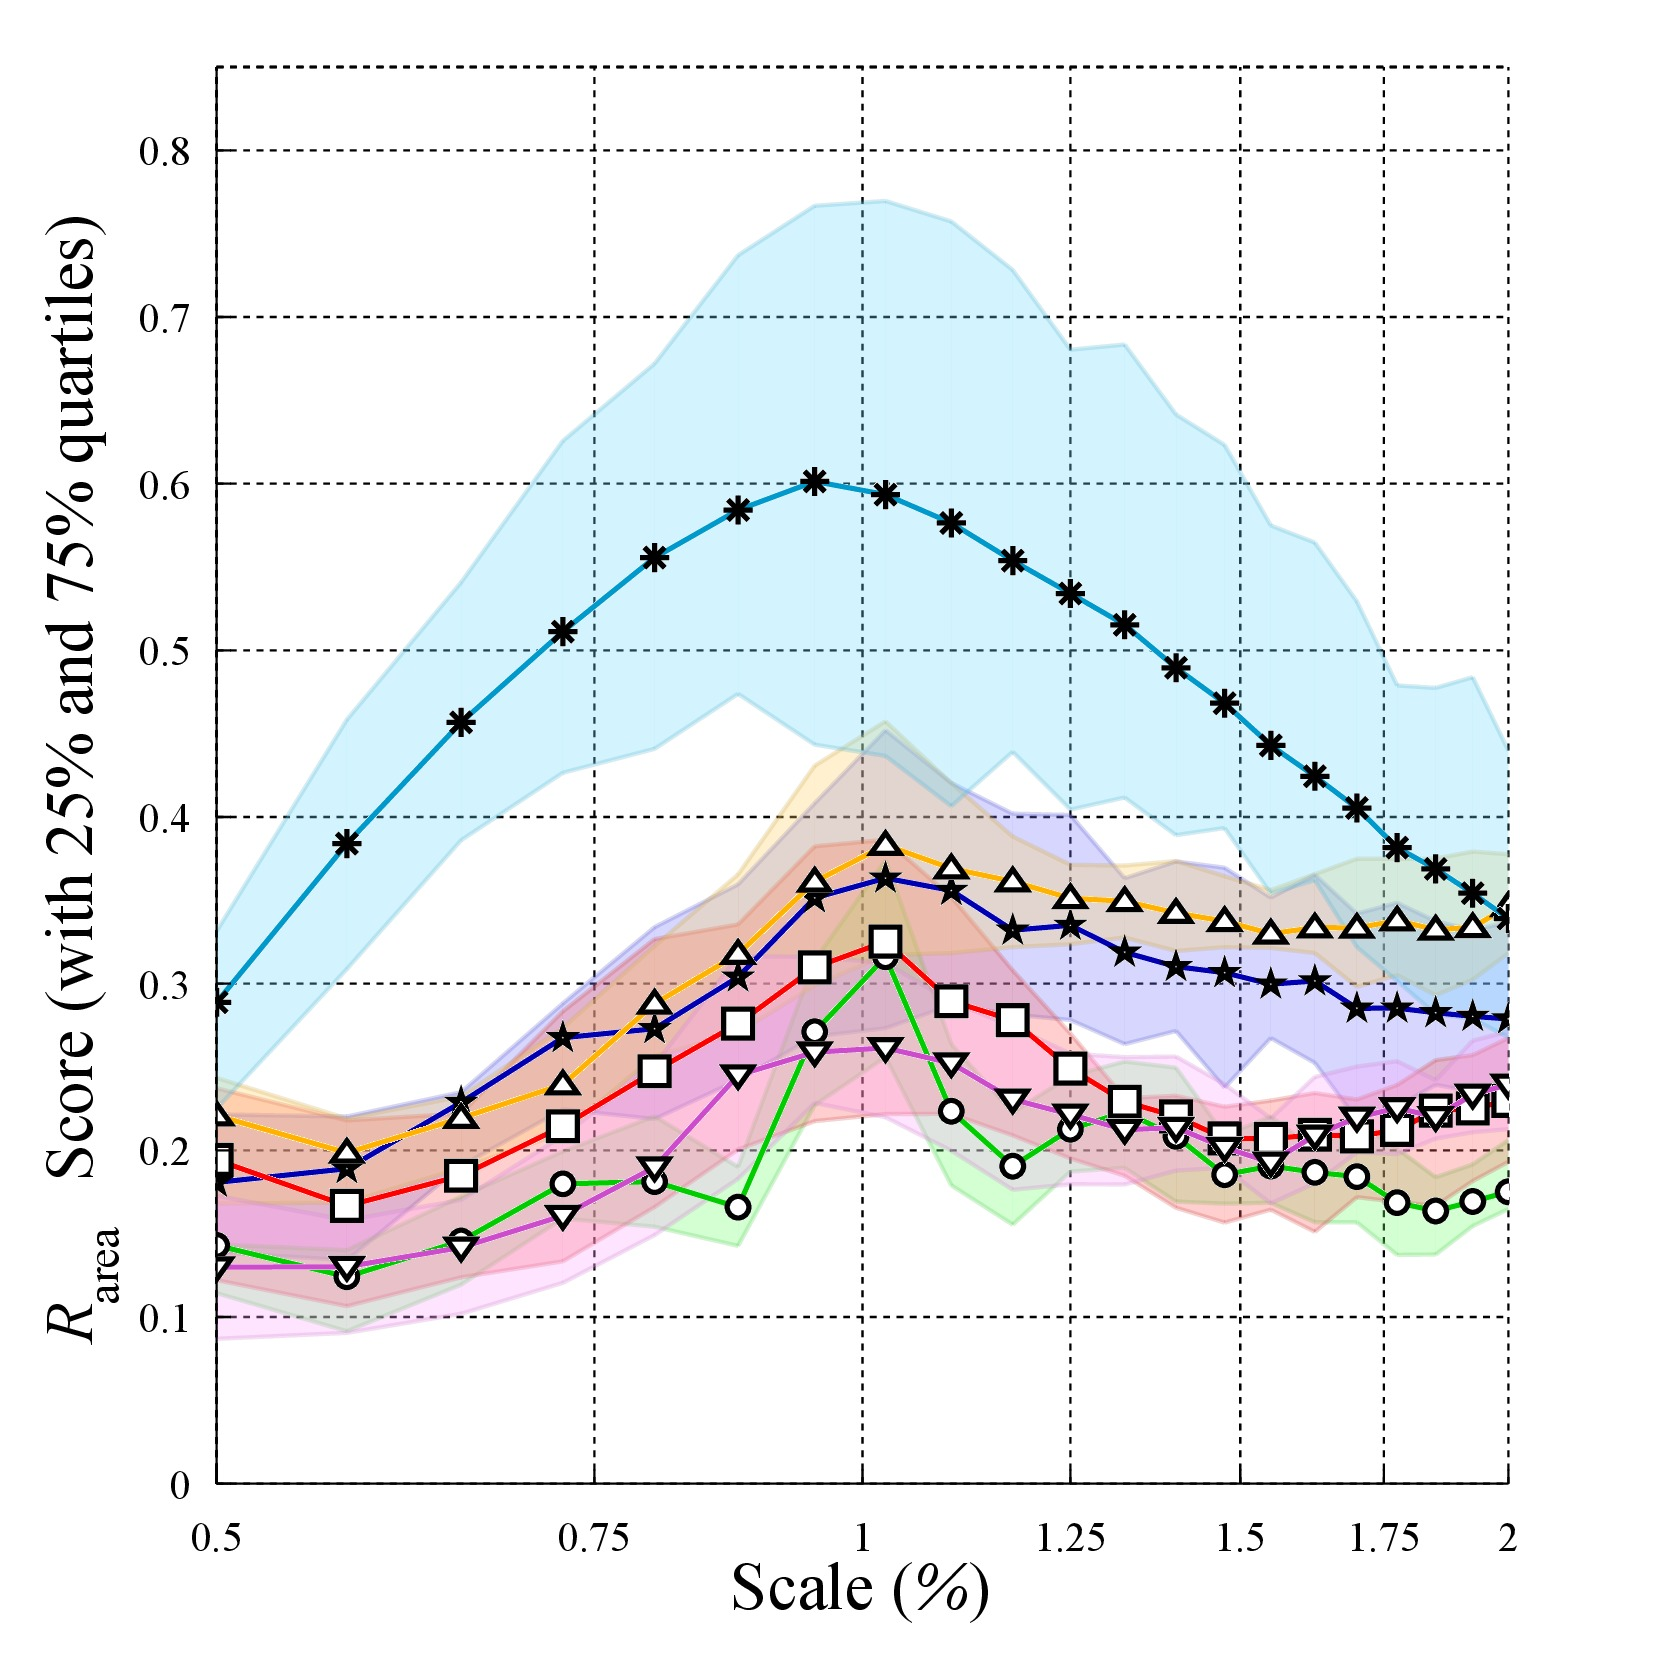
\includegraphics[width=0.35\linewidth]{./fig/eval/graph_scaling.jpg}
}
\subfloat[Percentage of Interest Points]{
	\label{fig:graph_keypointnum}
	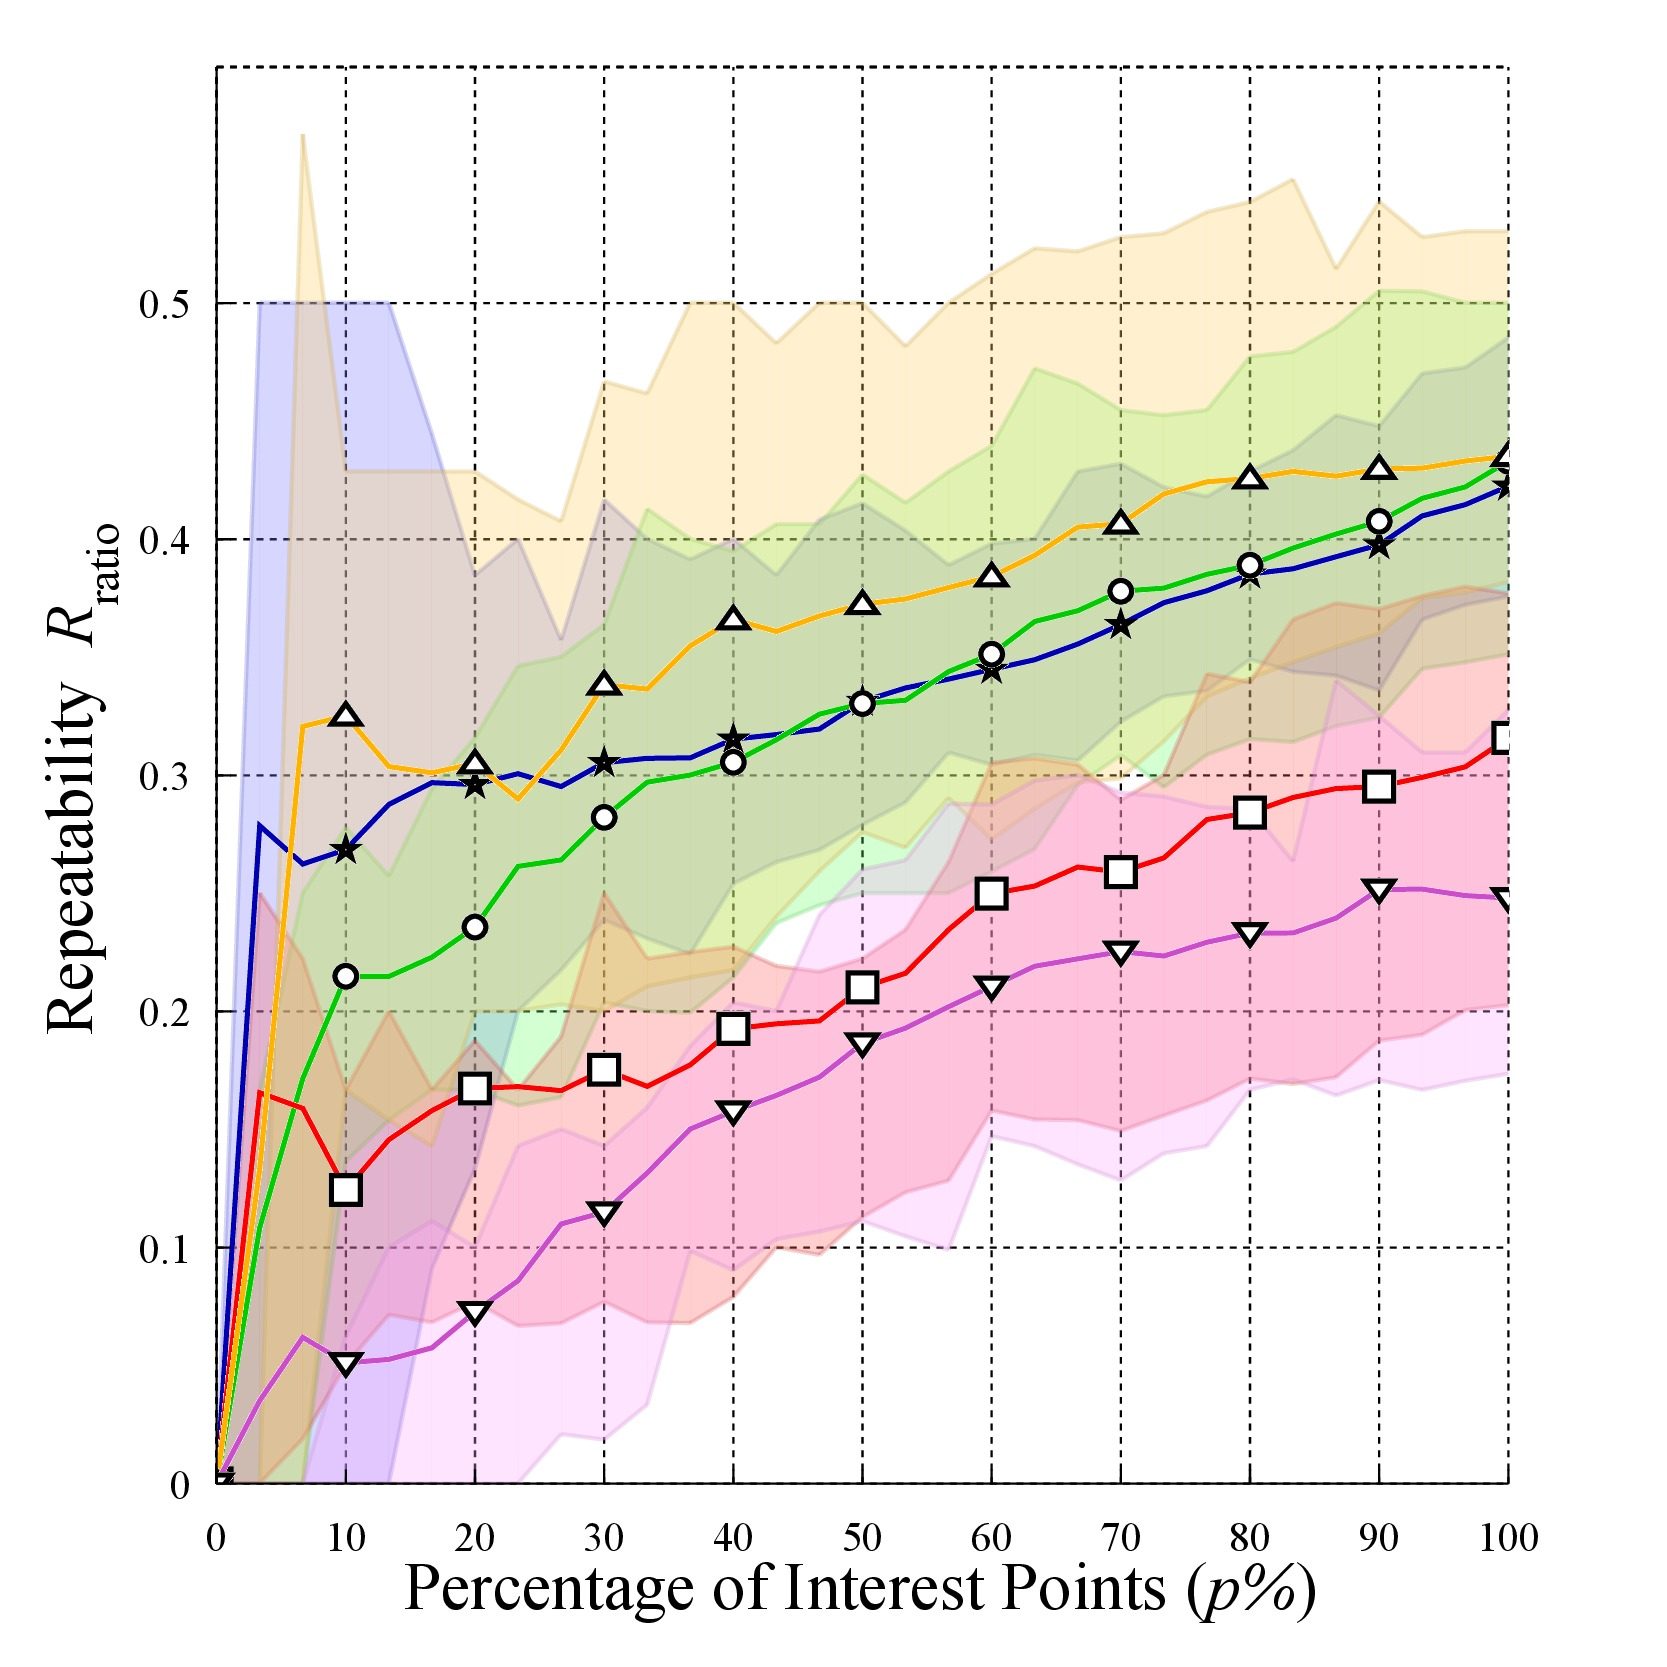
\includegraphics[width=0.35\linewidth]{./fig/eval/graph_keypointnum.jpg}
}
\caption{$R_{\textrm{area}}$ scores of \textbf{Mesh} dataset under changing (a) \emph{sampling noise}, (b) \emph{sampling density (point cloud size)}, (c) \emph{rotation}, (d) \emph{scale} and (e) \emph{percentage of detected interest points with highest saliency}. Solid lines indicate the average $R_{\textrm{area}}$ score.}
\label{fig:graph_graph0}
\end{figure}

Table~\ref{tab:numcorr} presents quantitative statistics for the number of interest points and correspondences at three noise levels ($0.0025$, $0.01$ and $0.02$ of $L$). Figure \ref{fig:noisesample} visualizes the effect of different sampling noise levels on the ``galleon'' shape in the \textbf{Mesh} dataset. The MSER detector has the highest percentage of correspondences, yet it gives a smaller set of interest points. By contrast, DoH, SURF and Harris produce larger sets of interest points with good correspondence ratios. The displacement threshold used here ($D = 0.015L$) is about half the typical value, hence only accurate correspondences are counted towards the values in the table. 

\subsubsection{Saliency}

Figure~\ref{fig:graph_keypointnum} shows the repeatability, $R_\textrm{ratio}$, with varying percentages of interest points. For each detector, the detected interest points are sorted by their corresponding saliency responses in descending order, then the first $p\%$ of interest points are used to calculate $R_\mathrm{ratio}$. However, since no saliency measure is defined in the MSER detector, the number of detected interest points cannot be controlled directly; MSER is therefore not included in figure \ref{fig:graph_keypointnum}. For analyzing the accuracies of the candidate detectors, $R_\textrm{ratio}$ is computed using a smaller displacement threshold ($D = 0.015L$) in this experiment.   

The performance of DoG and Harris detectors tend to be stable (though Harris performs notably worse than DoG) with increasing numbers of interest points (\ie decreasing saliency threshold), indicating that a saliency threshold is not necessary for these detectors. DoH's performance, which is initially the best, decreases very slowly and converges with DoG and SURF, indicating that the lower saliency points are less reliable. A saliency threshold for DoH might benefit applications requiring more accurate point localization. By contrast, the reapeatability scores of SURF and V-FAST increase steadily before leveling off, suggesting that some of the high saliency points are unreliable; this poses more of a problem in terms of interest point selection. 

\subsection{Experiments on MRI and stereo data}

\begin{figure}[ht]
\vspace{-2mm}
\centering
\subfloat[MRI scan 1]{
	\label{fig:mri1}
	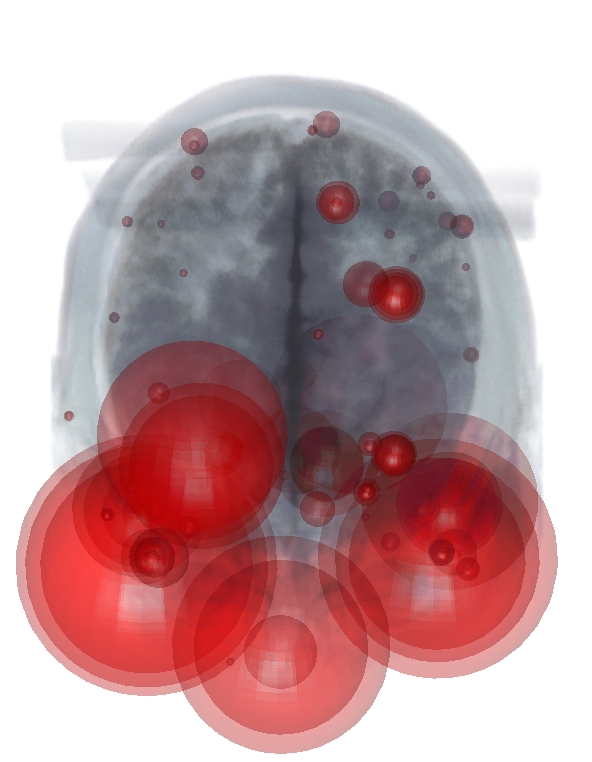
\includegraphics[width=0.45\linewidth]{./fig/eval/mri.png}
} 
\subfloat[MRI scan 2]{
	\label{fig:mri2}
	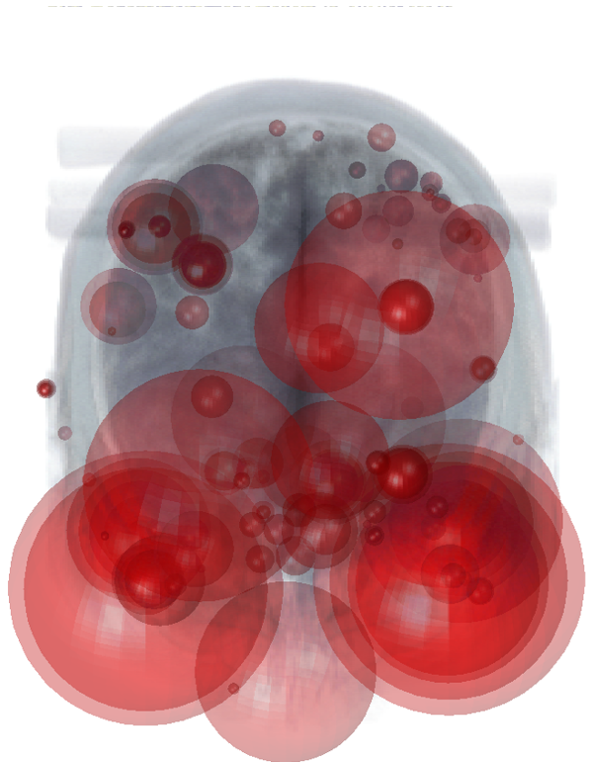
\includegraphics[width=0.45\linewidth]{./fig/eval/mri2.png}
}
\caption{Two volumetric MRI scans of a human brain, with detected MSER features.}
\label{fig:mri}
\vspace{-2mm}
\end{figure}

Interest points detectors are also evaluated on the {\textbf MRI} and {\textbf Stereo} datasets.
As a reference for cross validation, average scores obtained from the {\textbf Mesh} dataset are plotted against displacement threshold $d$ in figure \ref{fig:graph_syn}. 
  
\subsubsection{MRI dataset} This dataset contains two MRI scans of a human brain; each MRI has the longest dimension $L$ of $218$ voxels.
Figure \ref{fig:mri} shows the MSER interest points detected in the data. It is worth noting that some points detected on the MRIs can be matched easily, such as those on the nose-tips, eye sockets and foreheads, but that there are fewer detections within the brain area.

$R_{\textrm{area}}$ scores are measured from the dataset with varying $d$ in figure \ref{fig:graph_mri}. The evaluation results obtained are comparable to that of synthetic mesh data. MSER, DoG and DoH perform slightly better in synthetic meshes, while the Harris detector is good at detecting complicated internal structures in the MRI scans. 

\subsubsection{Stereo dataset} 
Sixteen point clouds,
generated using a multi-view stereo technique~\cite{Vogiatzis2011},
%from the Toshiba CAD dataset~\cite{Pham2011}
are converted into volumes with maximum length of $132$ voxels. Figure \ref{fig:mvs} shows some sample point clouds from the \textbf{Stereo} dataset and different interest points detected on their corresponding voxelized shapes.
The $R_{\textrm{area}}$ scores obtained from the {\textbf Stereo} dataset, shown in figure \ref{fig:graph_mvs}, are lower compared with {\textbf Mesh} and {\textbf MRI} datasets, especially at small $D$. Nonetheless, in terms of overall rankings and relative scores of the detectors, our synthetic and real data demonstrate similar behaviour. The decrease in performance for our stereo data could be due to its: \emph{(a)} low sampling frequency and high noise, \emph{(b)} uneven object surfaces, which are infeasible for blob detection algorithms (\eg MSER, SURF and DoH) and \emph{(c)} small errors in the estimated ground truth poses from ICP alignment.
The differences in $R_{\textrm{area}}$ scores are due to \emph{occlusions} due to viewpoint changes and \emph{uneven sampling density} of the {\textbf Stereo} data. 
 
Some objects (\eg ``mini'' in figure \ref{fig:mvs}) exhibit a much sparser reconstruction due to a lack of texture on the object's surface, but it is interesting to note that the distribution of detected features is no less dense across any of the detectors, suggesting that our synthetic results are representative of sparse point clouds as well as dense.

\begin{figure}[ht]
\centering
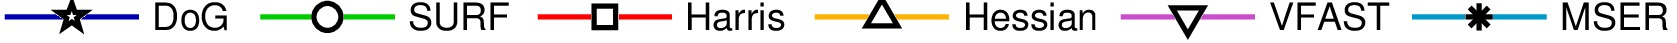
\includegraphics[width=0.80\linewidth]{./fig/eval/hlegend.jpg}\\
\vspace{-4mm}
\subfloat[$R_\textrm{area}$ score: \textbf{Mesh}]{
	\label{fig:graph_syn}
	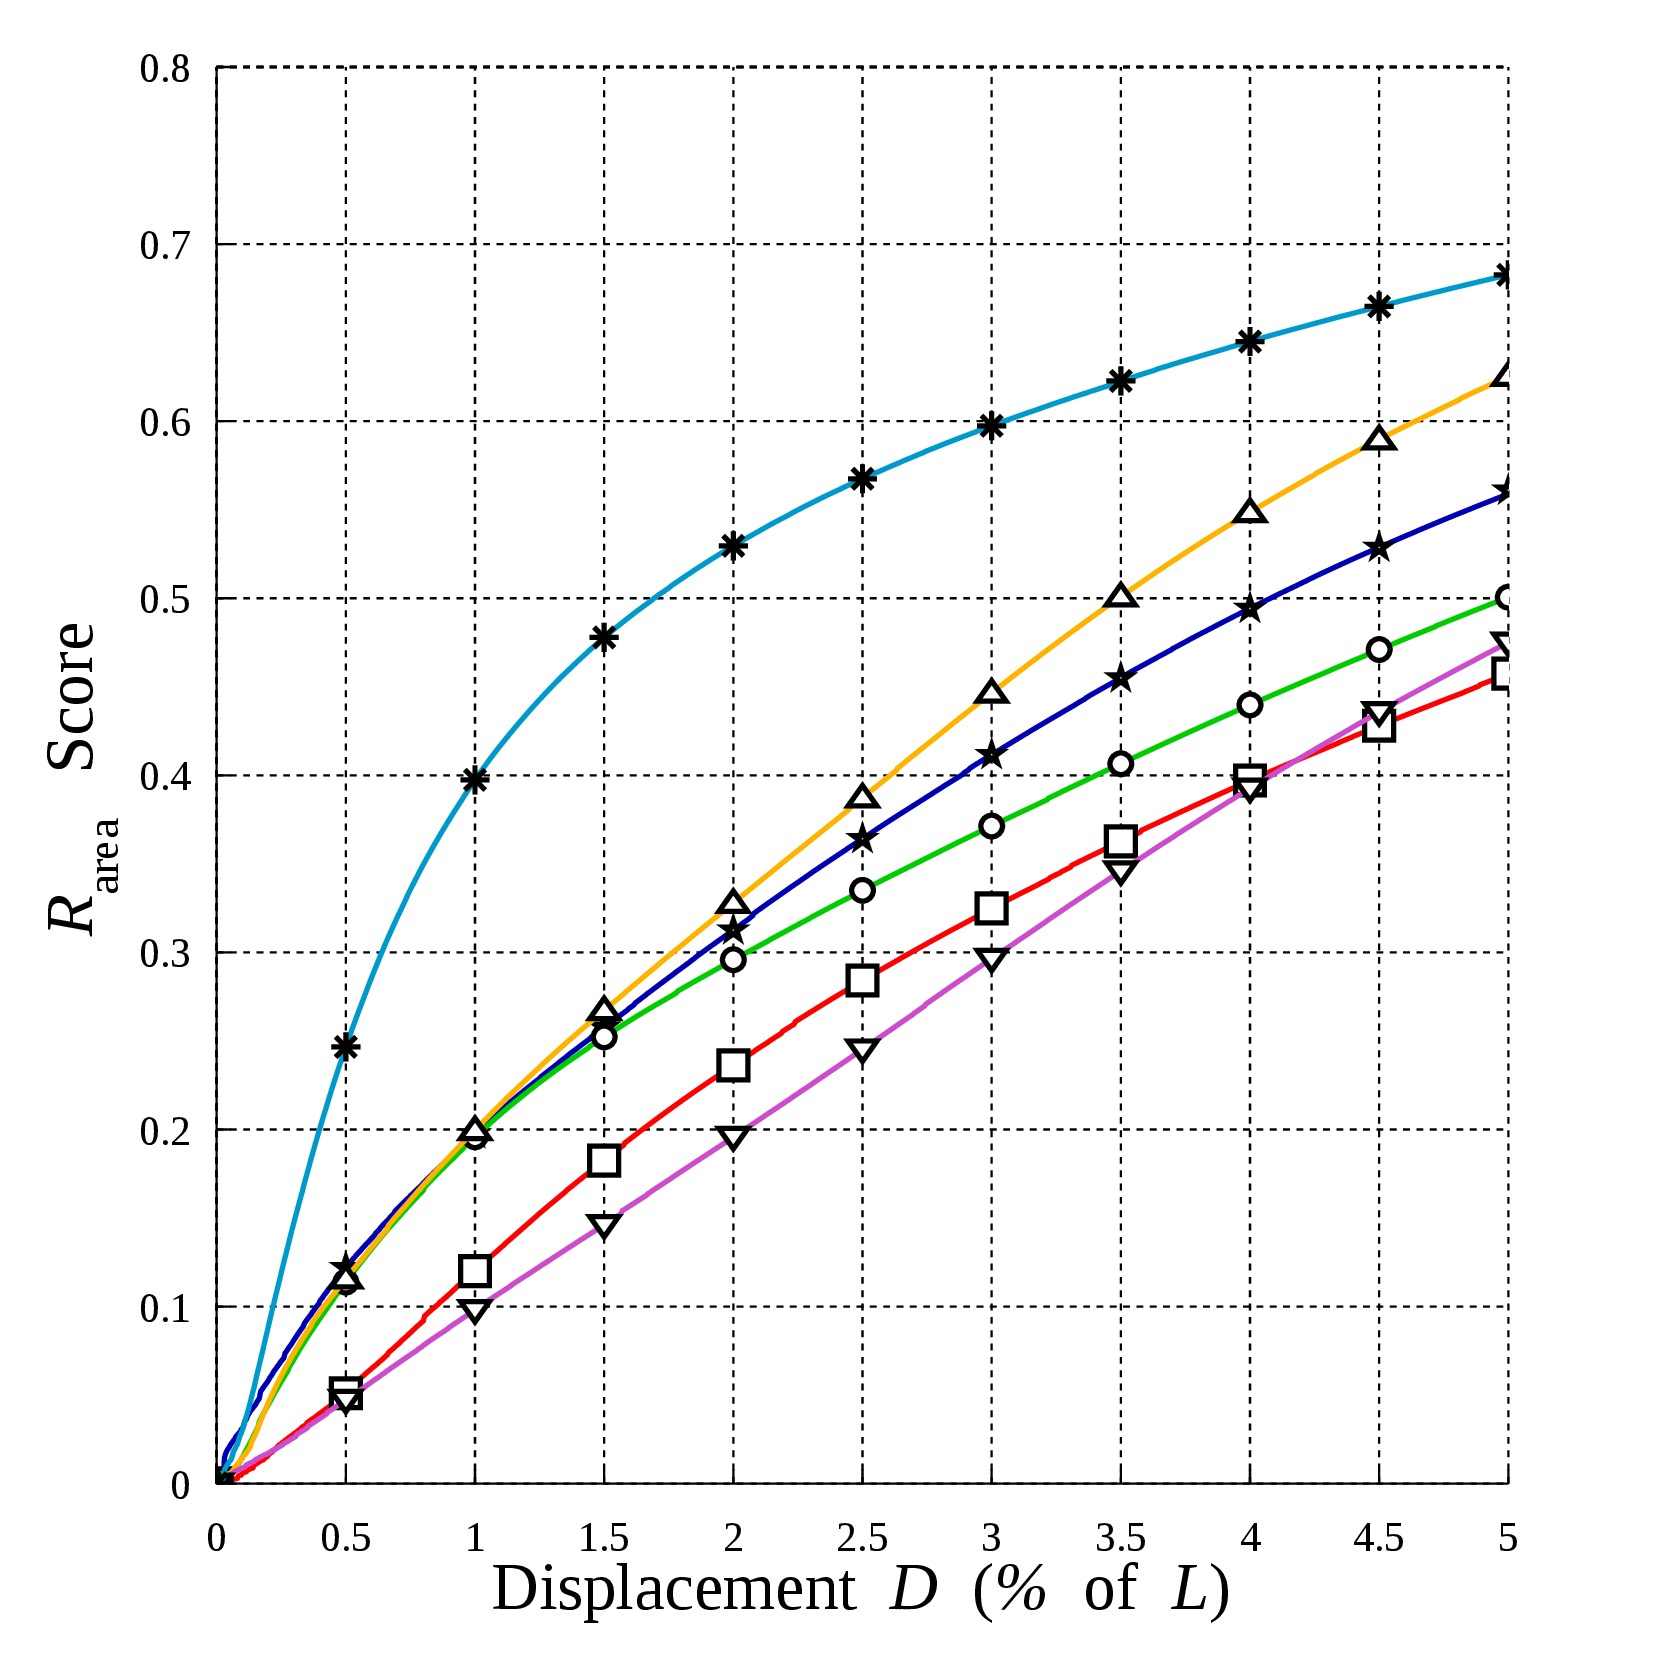
\includegraphics[width=0.33\linewidth]{./fig/eval/graph_oneshape.jpg}
}
\subfloat[$R_\textrm{area}$ score: \textbf{MRI}]{
	\label{fig:graph_mri}
	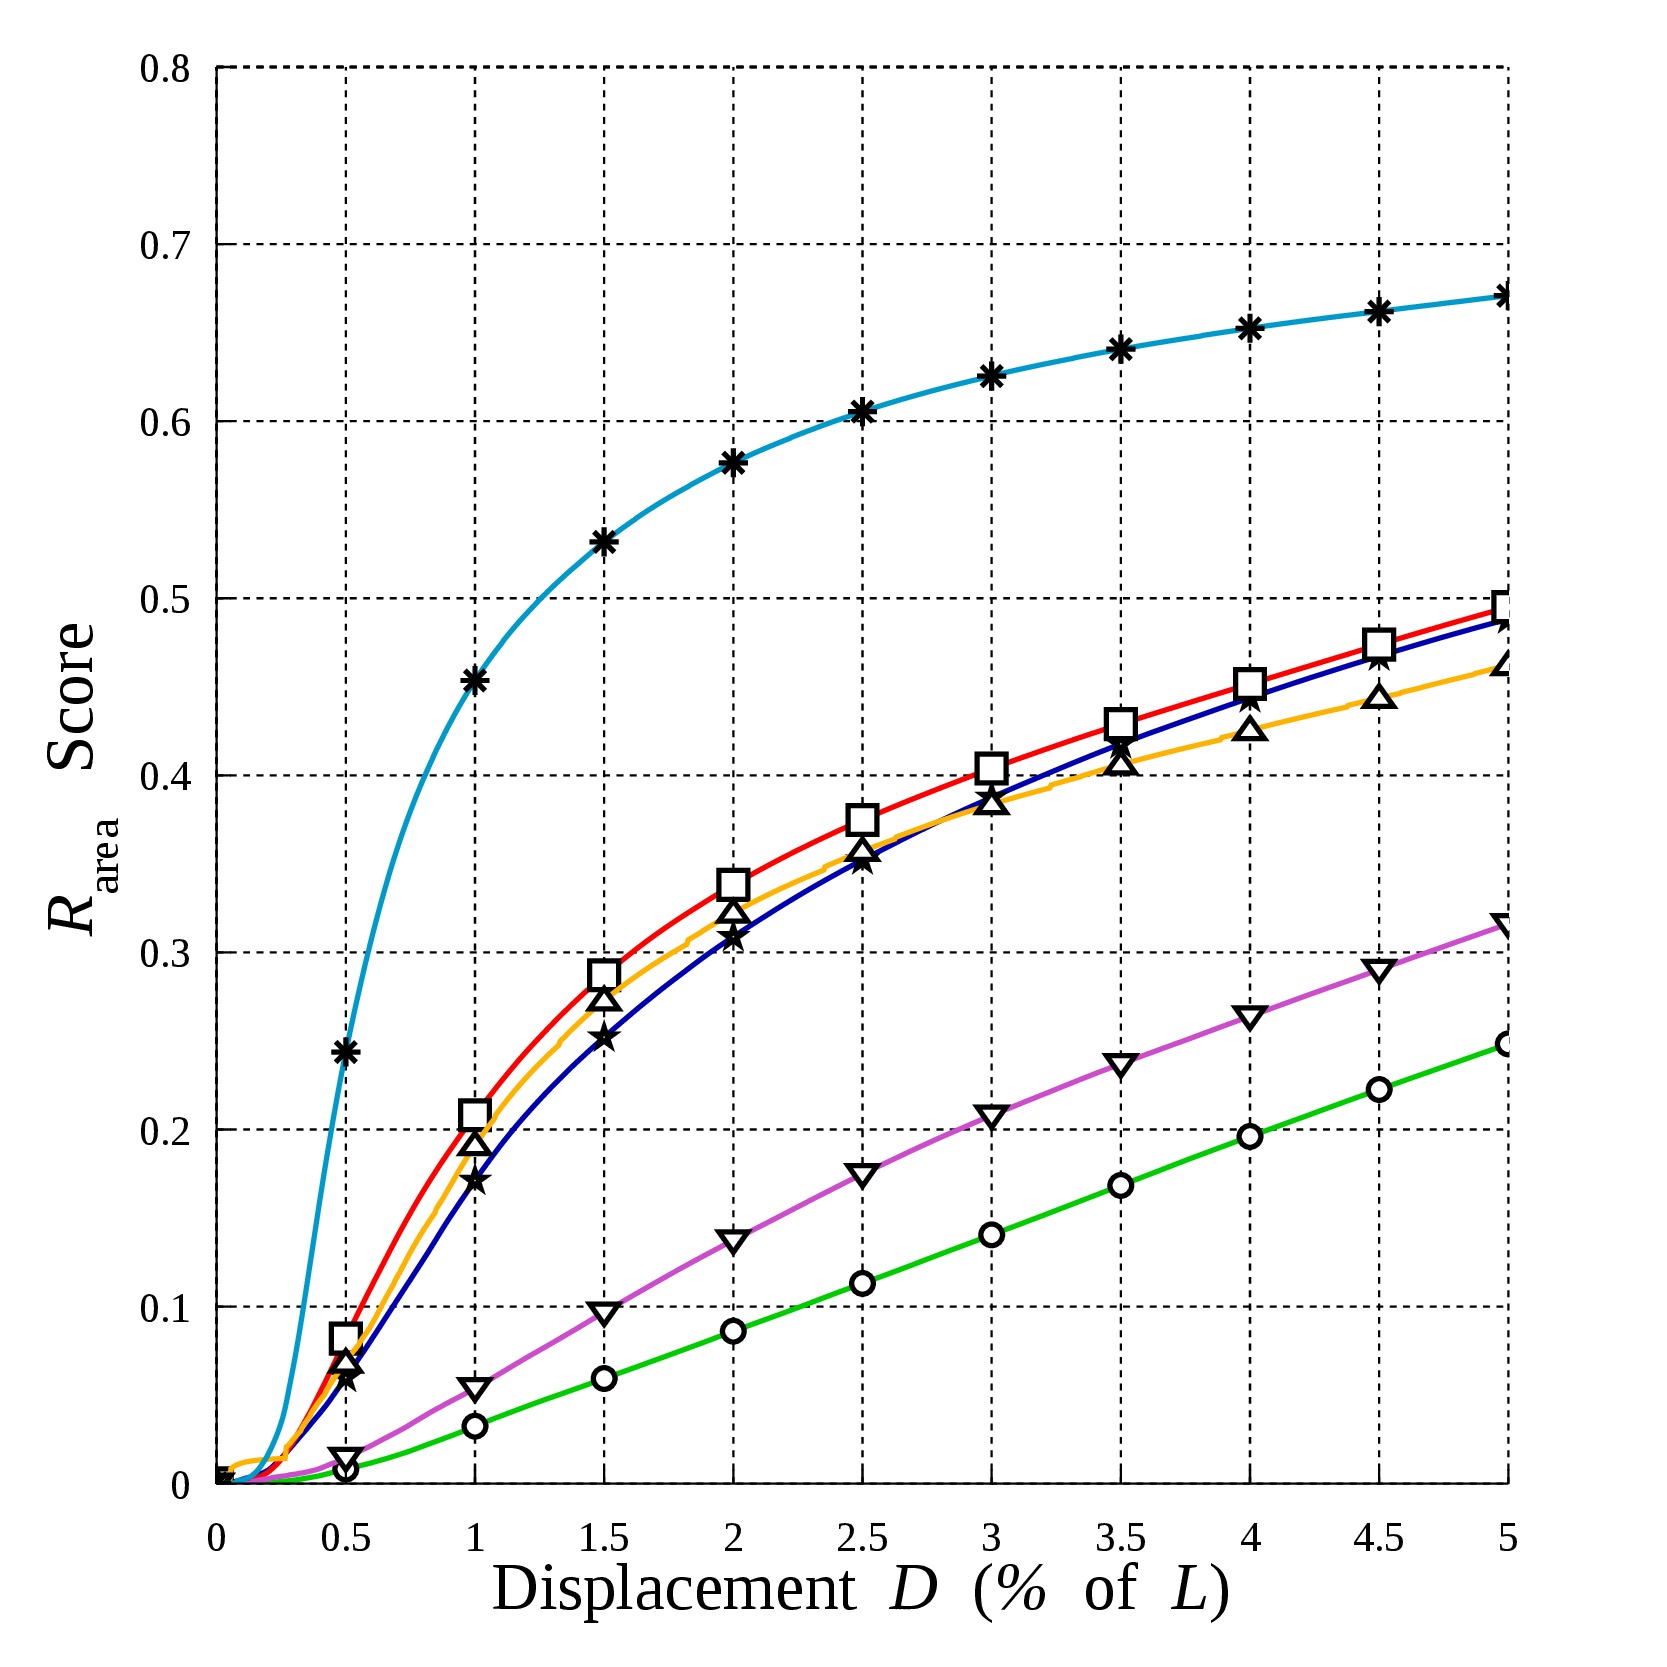
\includegraphics[width=0.33\linewidth]{./fig/eval/graph_mri.jpg}
}
\subfloat[$R_\textrm{area}$ score: \textbf{Stereo}]{
	\label{fig:graph_mvs}
	\includegraphics[width=0.33\linewidth]{./fig/eval/graph_stereo.jpg}
}
\caption{$R_{\textrm{area}}$ scores versus displacement threshold $d$. \emph{Left to right:} (a) {\textbf Mesh}, (b) {\textbf MRI} and (c) {\textbf Stereo} datasets.}
\label{fig:graph2}
\end{figure}

\subsection{Computation time}
Computation efficiency is also a crucial factor for choosing a suitable interest point detector for a particular computer vision application. Since the storage size of volumetric data is usually much larger than 2D images, the time required to compute the interest points increases accordingly. Operations which are considered efficient for 2D images may become much slower for 3D volumetric data. For non-volumetric data such as point clouds, extra computation time is required to voxelize the shape data. On the other hand, some interest point detectors can be accelerated by parallel processing techniques, using specialized hardware (\eg GPUs and FPGAs). Table \ref{tab:speedtable} summarizes the algorithmic complexities of the candidate detectors and the time required for them to compute interest points on the \textbf{Mesh} dataset. In order to compare the speed performance in a common evaluation framework, we implemented the all candidate detectors in MATLAB, without any hardware acceleration. The experiments were performed on the same hardware platform (Intel Core i7, $12$GB RAM). 
\begin{table*}
\centering
\begin{tabular}{c|cccc}
\hline
\textbf{Interest Point} & \textbf{Complexity} & \textbf{Speed ($\mu$s / voxel)} & \textbf{Parallelizable} & \textbf{Machine learning acceleration} \\
\hline
\textbf{DoG} 		& $O(SN)$ 			& $1.325 $ 			& \checkmark \cite{Sinha2006} & \\
\textbf{SURF} 		& $O(SN)$ 			& $1.035 $ 			& \checkmark \cite{Cornelis2008} & \\
\textbf{Harris} 	& $O(SN)$ 			& $1.112 $ 			& \checkmark \cite{Teixeira2008} & \\
\textbf{DoH} 		& $O(SN)$ 			& $1.325 $ 			& \checkmark \cite{Bhatia2007} \\
\textbf{V-FAST} 	& $O(SN)$ 			& $1.670 $ 			& \checkmark \cite{Dohi2011} & \checkmark \cite{Rosten2010}\\
\textbf{MSER} 		& $O(N\log\log N)$ 	& $2.070 $ 			& \checkmark \cite{Kristensen2007} &\\
\hline
\end{tabular}
\caption{\emph{From left to right:} the algorithmic complexities, the average time (in microseconds per voxel) to detect interest points on the \textbf{Mesh} dataset, the potential for heavily parallel implementation (with their corresponding 2D implementations as references), and the potential for machine learning based acceleration. $N$ is the number of voxels and $S$ is the number of octaves in the scale-space.}
\label{tab:speedtable}
\end{table*}
Theoretically all detectors have a similar time complexity, except for MSER, which does not implement a Gaussian scale-space. The SURF detector is the fastest among the candidate detectors, as it uses Haar wavelets to accelerate the computation of Gaussian derivatives. Harris also shows high efficiency due to its relatively simple algorithm. MSER is the slowest detector, as the search algorithm for stable regions is less efficient in 3D volumes than in 2D images. Surprisingly, the V-FAST detector is the second slowest detector in the experiment. Since FAST is a pixel/voxel-wise rule based algorithm, the accelerated segment test in equation \ref{eq:fastast} cannot utilize the high performance linear algebra routines used by other detectors such as DoG and SURF. On the other hand, the FAST detector can be accelerated by learning a decision tree classifier from training data \cite{Rosten2010}, which our implementation does not use.

\subsection{Qualitative analysis: Blobs versus Corners}
Volumetric interest points can be roughly classified into three categories: region-based blob detection (MSER), derivative-based blob detection (DoG, DoH and SURF) and corner detection (Harris, V-FAST). The quantitative evaluation results imply that region-based blob detectors work better than derivative-based blob detectors, and blob detectors are better than corner detectors, but this is not the whole story. The candidate detectors demonstrate different behaviours in terms of locations and scales of the detected interest points. Therefore, besides repeatability, it is also important to analyze the characteristics of detectors qualitatively. Figure \ref{fig:mesh} visualizes interest points detected by the six candidate detectors on the ``cat'' object from the {\textbf Mesh} dataset.

\subsubsection{Region-based blob detection} MSER detects contiguous regions of any shape (\ie not limited to spherical blobs) allowing it to select more robust regions from a greater selection, and hence perform better. MSER performs well in 3D shape data because the shapes of salient regions are inherently less susceptible to viewpoint changes. It can be seen in figures \ref{fig:mesh:mser} and \ref{fig:mvs:mser} that MSER finds features at fewer locations, but over multiple scales. The locations tend to center on regions of high surface curvature.

\subsubsection{Derivative-based blob detection} DoG, DoH and SURF detectors theoretically find, in order of preference, spherical blobs, corners and planes. DoG and DoH have qualitatively similar output, as shown in figures \ref{fig:mesh:dog}, \ref{fig:mvs:dog}, \ref{fig:mesh:hessian} and \ref{fig:mvs:hessian}, finding features such as limb extremities in \textbf{Mesh} dataset or sharp corners in \textbf{Stereo} dataset, as well as inside shape such as the hull of ``galleon'' and the hole in ``knob''. By contrast, SURF (figure \ref{fig:testshapes:surf}), despite being an approximation of the DoH detector, produces features off the surface (both inside and outside), often over regions of low surface curvature. Instead of highly repeatable features, derivative-based approaches produce qualitatively more diverse features than region-based detectors. Finally, their repeatability scores degrade more rapidly than MSER for noisy input data (see figure~\ref{fig:graph_noise}), mainly due to higher rates of false positive detections. 

\subsubsection{Corner detection} Harris and V-FAST both aim to find areas of high curvature. However, their outputs (figures \ref{fig:testshapes:harris} and \ref{fig:testshapes:fast}) vary qualitatively, with the former tending to find fewer features and more sharp corners than the latter, which finds an even distribution of features over both scale and location. In general, corner detection approaches are relatively less robust to noise and transformations than blob detection techniques. Whilst blobs remain stable in noisy or transformed volumetric data, corners are more easily affected by quantization errors or sampling noise. 
The performance of blob detectors drops faster than that of edge detectors at low (see figure \ref{fig:graph_sample}) and uneven (compare figures \ref{fig:graph_syn} and \ref{fig:graph_mvs}) sampling densities. Holes form on shape surfaces in these situations, creating false positives for both corner and blob detectors, but the detection of true positives appears to be more robust for corner detectors in these cases. 
% Comparing the \textbf{Mesh} dataset and the \textbf{Stereo} dataset, blob detectors have a greater drop in $R_{\textrm{area}}$ score than corner detectors. It is because holes are formed on shape surfaces at a low or uneven sampling density, \eg \textbf{Stereo} dataset in figure \ref{fig:mvs}, they prevent the formation of stable blobs inside the cavities of a shape as in the \textbf{Mesh} dataset (figure \ref{fig:mesh}). On the other hand, corner features are mainly detected at edges where the sampling density is generally higher than shape surfaces, thus they are less affected. Nevertheless, the unevenly sampled surface create false positives for all detectors, an overall drop in $R_{\textrm{area}}$ score is therefore observed in \ref{fig:mvs}. 
%Holes are formed on the shapes' surfaces at a low or uneven sampling density, \eg \textbf{Stereo} dataset in figure \ref{fig:graph_mvs}, creating false positives for both corner and blob detectors. These holes also prevents the formation of larger blobs. However, detection of corner features, which are usually smaller in size than blobs, are less affected. 
%On the other hand, since corner-based detectors use smaller local windows than blob-based methods, they are feasible for detecting interest points when blobs cannot be detected correctly in low sampling density (\emph{c.f.} figure \ref{fig:graph_mvs}).

\begin{figure}[ht]
	\centering
	\begin{subfigure}[t]{1\linewidth}\centering
		\makebox[0.15\linewidth]{}
		\makebox[0.175\linewidth]{\textbf{Bicycle}}
		\makebox[0.155\linewidth]{\textbf{Kicking man}}
		\makebox[0.175\linewidth]{\textbf{Galleon}}
		\makebox[0.175\linewidth]{\textbf{Ant}}
	\end{subfigure}
	\begin{subfigure}[t]{1\linewidth} \centering 
		\phantomcaption 
		\label{fig/eval/mesh/input}	
		\makebox[0.15\linewidth]{\raisebox{0.07\linewidth}{(a) Input}} 
		\includegraphics[width=0.175\linewidth]{./fig/eval/cycle_input.jpg} 
		\includegraphics[width=0.155\linewidth]{./fig/eval/guy_input.jpg} 
		\includegraphics[width=0.175\linewidth]{./fig/eval/ship_input.jpg}
		\includegraphics[width=0.175\linewidth]{./fig/eval/ant_input.jpg} 
	\end{subfigure}
	\begin{subfigure}[t]{1\linewidth} \centering 
		\phantomcaption 
		\label{fig/eval/mesh/dog}	
		\makebox[0.15\linewidth]{\raisebox{0.07\linewidth}{(b) DoG}} 
		\includegraphics[width=0.175\linewidth]{./fig/eval/cycle_dog.jpg} 
		\includegraphics[width=0.155\linewidth]{./fig/eval/guy_dog.jpg} 
		\includegraphics[width=0.175\linewidth]{./fig/eval/ship_dog.jpg}
		\includegraphics[width=0.175\linewidth]{./fig/eval/ant_dog.jpg} 
	\end{subfigure}
	\begin{subfigure}[t]{1\linewidth} \centering 
		\phantomcaption 
		\label{fig/eval/mesh/surf}	
		\makebox[0.15\linewidth]{\raisebox{0.07\linewidth}{(c) SURF}} 
		\includegraphics[width=0.175\linewidth]{./fig/eval/cycle_surf.jpg} 
		\includegraphics[width=0.155\linewidth]{./fig/eval/guy_surf.jpg} 
		\includegraphics[width=0.175\linewidth]{./fig/eval/ship_surf.jpg}
		\includegraphics[width=0.175\linewidth]{./fig/eval/ant_surf.jpg} 
	\end{subfigure}
	\begin{subfigure}[t]{1\linewidth} \centering 
		\phantomcaption 
		\label{fig/eval/mesh/harris}	
		\makebox[0.15\linewidth]{\raisebox{0.07\linewidth}{(d) Harris}} 
		\includegraphics[width=0.175\linewidth]{./fig/eval/cycle_harris.jpg} 
		\includegraphics[width=0.155\linewidth]{./fig/eval/guy_harris.jpg} 
		\includegraphics[width=0.175\linewidth]{./fig/eval/ship_harris.jpg}
		\includegraphics[width=0.175\linewidth]{./fig/eval/ant_harris.jpg} 
	\end{subfigure}
	\begin{subfigure}[t]{1\linewidth} \centering 
		\phantomcaption 
		\label{fig/eval/mesh/hessian}	
		\makebox[0.15\linewidth]{\raisebox{0.07\linewidth}{(e) DoH}} 
		\includegraphics[width=0.175\linewidth]{./fig/eval/cycle_hessian.jpg} 
		\includegraphics[width=0.155\linewidth]{./fig/eval/guy_hessian.jpg} 
		\includegraphics[width=0.175\linewidth]{./fig/eval/ship_hessian.jpg}
		\includegraphics[width=0.175\linewidth]{./fig/eval/ant_hessian.jpg} 
	\end{subfigure}
	\begin{subfigure}[t]{1\linewidth} \centering 
		\phantomcaption 
		\label{fig/eval/mesh/fast}	
		\makebox[0.15\linewidth]{\raisebox{0.07\linewidth}{(f) VFAST}} 
		\includegraphics[width=0.175\linewidth]{./fig/eval/cycle_fast.jpg} 
		\includegraphics[width=0.155\linewidth]{./fig/eval/guy_fast.jpg} 
		\includegraphics[width=0.175\linewidth]{./fig/eval/ship_fast.jpg}
		\includegraphics[width=0.175\linewidth]{./fig/eval/ant_fast.jpg} 
	\end{subfigure}
	\begin{subfigure}[t]{1\linewidth} \centering 
		\phantomcaption 
		\label{fig/eval/mesh/mser}	
		\makebox[0.15\linewidth]{\raisebox{0.07\linewidth}{(g) MSER}} 
		\includegraphics[width=0.175\linewidth]{./fig/eval/cycle_mser.jpg} 
		\includegraphics[width=0.155\linewidth]{./fig/eval/guy_mser.jpg} 
		\includegraphics[width=0.175\linewidth]{./fig/eval/ship_mser.jpg}
		\includegraphics[width=0.175\linewidth]{./fig/eval/ant_mser.jpg} 
	\end{subfigure}
	\caption{(a) Sample point clouds obtained from the Mesh dataset, (b) DoG, (c) SURF (d) Harris, (e) DoH, (f) V-FAST and (g) MSER, visualized on the voxelized data. The color spheres represent the positions and relative scales of the detected interest points.}
	\label{fig/eval/mesh}
\end{figure}


\begin{figure}[ht]
	\centering 
	\begin{subfigure}[t]{1\linewidth} \centering
		\makebox[0.15\linewidth]{}
		\makebox[0.180\linewidth]{\textbf{Car}}
		\makebox[0.180\linewidth]{\textbf{Bearing}}
		\makebox[0.180\linewidth]{\textbf{Knob}}
		\makebox[0.180\linewidth]{\textbf{Bracket}}
	\end{subfigure}
	\begin{subfigure}[t]{1\linewidth} \centering
		\phantomcaption 
		\label{fig/eval/mvs/input}
		\makebox[0.15\linewidth]{\raisebox{0.07\linewidth}{(a) Input}}		
		\includegraphics[width=0.180\linewidth]{./fig/eval/mini_input.jpg}
		\includegraphics[width=0.180\linewidth]{./fig/eval/bearing_input.jpg} 
		\includegraphics[width=0.180\linewidth]{./fig/eval/knob_input.jpg} 
		\includegraphics[width=0.180\linewidth]{./fig/eval/bracket_input.jpg} 
	\end{subfigure}
	\begin{subfigure}[t]{1\linewidth} \centering
		\phantomcaption 
		\label{fig/eval/mvs/dog}
		\makebox[0.15\linewidth]{\raisebox{0.07\linewidth}{(b) DoG}} 
		\includegraphics[width=0.180\linewidth]{./fig/eval/mini_dog.jpg} 
		\includegraphics[width=0.180\linewidth]{./fig/eval/bearing_dog.jpg}  
		\includegraphics[width=0.180\linewidth]{./fig/eval/knob_dog.jpg} 
		\includegraphics[width=0.180\linewidth]{./fig/eval/bracket_dog.jpg} 
	\end{subfigure}
	\begin{subfigure}[t]{1\linewidth} \centering
		\phantomcaption 
		\label{fig/eval/mvs/surf}
		\makebox[0.15\linewidth]{\raisebox{0.07\linewidth}{(c) SURF}}		
		\includegraphics[width=0.180\linewidth]{./fig/eval/mini_surf.jpg} 
		\includegraphics[width=0.180\linewidth]{./fig/eval/bearing_surf.jpg}  
		\includegraphics[width=0.180\linewidth]{./fig/eval/knob_surf.jpg} 
		\includegraphics[width=0.180\linewidth]{./fig/eval/bracket_surf.jpg} 
	\end{subfigure}
	\begin{subfigure}[t]{1\linewidth} \centering
		\phantomcaption 
		\label{fig/eval/mvs/harris}
		\makebox[0.15\linewidth]{\raisebox{0.07\linewidth}{(d) Harris}}		
		\includegraphics[width=0.180\linewidth]{./fig/eval/mini_harris.jpg} 
		\includegraphics[width=0.180\linewidth]{./fig/eval/bearing_harris.jpg}  
		\includegraphics[width=0.180\linewidth]{./fig/eval/knob_harris.jpg} 
		\includegraphics[width=0.180\linewidth]{./fig/eval/bracket_harris.jpg} 
	\end{subfigure}
	\begin{subfigure}[t]{1\linewidth} \centering
		\phantomcaption 
		\label{fig/eval/mvs/hessian}
		\makebox[0.15\linewidth]{\raisebox{0.07\linewidth}{(e) Hessian}}		
		\includegraphics[width=0.180\linewidth]{./fig/eval/mini_hessian.jpg} 
		\includegraphics[width=0.180\linewidth]{./fig/eval/bearing_hessian.jpg}  
		\includegraphics[width=0.180\linewidth]{./fig/eval/knob_hessian.jpg} 
		\includegraphics[width=0.180\linewidth]{./fig/eval/bracket_hessian.jpg} 
	\end{subfigure}
	\begin{subfigure}[t]{1\linewidth} \centering
		\phantomcaption 
		\label{fig/eval/mvs/vfast}
		\makebox[0.15\linewidth]{\raisebox{0.07\linewidth}{(f) VFAST}}		
		\includegraphics[width=0.180\linewidth]{./fig/eval/mini_fast.jpg} 
		\includegraphics[width=0.180\linewidth]{./fig/eval/bearing_fast.jpg}  
		\includegraphics[width=0.180\linewidth]{./fig/eval/knob_fast.jpg} 
		\includegraphics[width=0.180\linewidth]{./fig/eval/bracket_fast.jpg} 
	\end{subfigure}
	\begin{subfigure}[t]{1\linewidth} \centering
		\phantomcaption 
		\label{fig/eval/mvs/mser}
		\makebox[0.15\linewidth]{\raisebox{0.07\linewidth}{(g) MSER}}	
		\includegraphics[width=0.180\linewidth]{./fig/eval/mini_mser.jpg} 
		\includegraphics[width=0.180\linewidth]{./fig/eval/bearing_mser.jpg}  
		\includegraphics[width=0.180\linewidth]{./fig/eval/knob_mser.jpg} 
		\includegraphics[width=0.180\linewidth]{./fig/eval/bracket_mser.jpg} 
	\end{subfigure}
	\caption{(a) Sample point clouds obtained from the stereo dataset. (b) DoG, (c) SURF (d) Harris, (e) DoH, (f) V-FAST and (g) MSER interest points visualized on the voxelized data.}
	\label{fig/eval/mvs}
\end{figure}



\section{Conclusion}
\label{sec:conclusion}
% What's done?
In this paper, the state of the art in volumetric interest point detection is evaluated. The purpose of this work is to provide comprehensive guidance on the selection of interest point detector for any computer vision or machine learning task that uses 3D input data. Six interest point detectors, from existing 3D computer vision applications, are evaluated on three different datasets (meshes, MRI scans and 3D point clouds) under varying noise levels and transformations. 
A novel evaluation metric is introduced by combining two existing performance metrics, repeatability and accuracy, into a single measurement. The acquired experimental results are analyzed both quantitatively and qualitatively.

% What's learnt / interesting? What to do next?
% First part is quantitative: MSER seems very nice?
% Second part is qualitative: Not really, there are many other factors that cannot be described quantitatively...
% Conclusion: "It depends. So please read our paper."

Summarizing the quantitative results with respect to the proposed $R_{\textrm{area}}$ score, MSER achieves the best overall performance, being robust to both noise and rotation. Taking the number of corresponding points into account, DoH and, to a lesser extent, DoG maintain a balanced performance between this and repeatability. Generally speaking, blob detectors (\eg DoH and DoG) appear to perform better than corner detectors (\eg Harris and V-FAST) in 3D shapes, a result that agrees with an evaluation of image-based detectors~\cite{Mikolajczyk2005}. Consistent results are obtained from different evaluation datasets, which indicate that both the detectors and evaluation framework are applicable to multiple types of input data. In the context of efficiency, MSER is the slowest interest point detector in terms of computation time for 3D volumetric data. Evaluation results show that fast detectors for 2D images, \eg FAST, may not obtain consistent performances for 3D volumes. Hardware acceleration is essential when real-time performance is needed. While parallelized, hardware-accelerated 2D interest points are available, volumetric implementations of such detectors are still uncommon. 

In the qualitative analysis we discussed the nature of features found by the candidate interest point detectors. They exhibit unique characteristics with respect to their locations, sizes and number of interest points. 
The analysis suggests that the repeatability of a detector is also affected by the nature of input data, such as the number of distinct corners, edges or blobs on the 3D shapes. In addition, the suitability of an interest point depends on the qualitative requirements of the target applications (\eg object classification, correspondence matching, segmentation). Hence, repeatability is not the sole factor in determining the performance of applications; the choice of volumetric interest points is actually application dependent. 
